\section{Continuous Integration/Delivery}
\subsection{GitHub Actions}

allg. actions warum kosten
\subsubsection{iOS Build}
\setauthor{Martin Hausleitner}
Das Ziel des Projekts war es, eine \href{https://www.apple.com/ios/app-store/}{iOS-App im App Store} zu veröffentlichen und eine \href{https://play.google.com/store/apps}{Android-App im Play Store} anzubieten. Da Martin Hausleitner der einzige im Team war, der ein iPhone besaß und Erfahrungen mit Apple hatte, übernahm er die Verantwortung für den Build-Prozess der iOS-App.

Zur Erstellung einer \href{https://flutter.dev/}{Flutter}
iOS-App ist ein Mac mit
\href{https://developer.apple.com/xcode/}{Xcode} sowie ein
\href{https://developer.apple.com/programs/}{Apple-Entwicklerkonto}
erforderlich. Da jedoch niemand im Team über ein solches
Konto verfügte, gestaltete sich der Build-Prozess äußerst
schwierig. Glücklicherweise konnte Martin Hausleitner einen
alten iMac von seiner Familie ausleihen, auf dem er arbeiten
konnte. Obwohl das Erstellen einer iOS-App auf den ersten
Blick einfach erscheint, stellte es sich als eine der
größten Herausforderungen in diesem Projekt heraus.

Da MacOS und Xcode dem Entwickler nicht vertraut waren, musste er sich zunächst mühsam einarbeiten. Es bedurfte zahlreicher Anläufe, um die App zum ersten Mal zu erstellen, da zum damaligen Zeitpunkt von Flutter noch keine vorgefertigten Build-Abläufe zur Verfügung standen.





\paragraph{Github Action}
Es war eine mühsame Aufgabe, Xcode zu konfigurieren, und
nach mehreren Versuchen wurde schließlich die erste
.ipa-Datei erstellt. Allerdings war der schwierigste Teil
noch nicht überwunden, da das Ziel darin bestand, bei jedem
GitHub-Push automatisch eine iOS-App zu erstellen.

Um über GitHub Actions eine iOS-App zu erstellen, sind
mehrere Actions-Secrets erforderlich, die aus Xcode bezogen
werden müssen. Folgende Secrets waren notwendig:

\begin{itemize}
  \item \verb|BUILD_CERTIFICATE_BASE64:| Dieses Secret enthält das Zertifikat, das zur Signierung der iOS-App verwendet wird. Es muss von einer vertrauenswürdigen Zertifizierungsstelle ausgestellt worden sein und wird normalerweise als Base64-codierte Zeichenfolge bereitgestellt.
  \item \verb|BUILD_PROVISION_PROFILE_BASE64:| Dieses Secret enthält das Provisioning-Profil, das zur Installation der iOS-App auf einem Gerät oder für die Verwendung von Testflight verwendet wird. Das Provisioning-Profil enthält Informationen über die Geräte, auf denen die App installiert werden kann, sowie das verwendete Zertifikat. Auch dieses Secret wird normalerweise als Base64-codierte Zeichenfolge bereitgestellt.
  \item \verb|KEYCHAIN_PASSWORD:| Dieses Secret ist das Passwort für den Zugriff auf den Schlüsselbund, in dem das Signaturzertifikat und der dazugehörige private Schlüssel gespeichert sind. Der private Schlüssel wird benötigt, um die App zu signieren, und das Passwort schützt den Zugriff auf den Schlüsselbund vor unbefugtem Zugriff.
  \item \verb|P12_PASSWORD:| Dieses Secret ist das Passwort für das PKCS\#12-Dateiformat, das das Signaturzertifikat und den privaten Schlüssel enthält. Diese Datei wird normalerweise für die Signierung von iOS-Apps verwendet. Das Passwort schützt die Datei vor unbefugtem Zugriff und stellt sicher, dass nur autorisierte Personen Zugriff auf den privaten Schlüssel haben.
\end{itemize}

Nach mehreren Versuchen, die Actions funktionsfähig zu
machen, gelang es schließlich, eine .ipa-Datei zu erstellen.

\paragraph{Firebase App Distribution}
Für die Testphase und die Beta-Version der iOS-App nutzten
wir, wie auch bei der Android-App, Firebase App
Distribution. Beim Hochladen der .ipa-Dateien gab es
allerdings Probleme mit den Zertifikaten.

\paragraph{Apple Developer Lizenz}
Um eine .ipa-Datei auf einem iOS-Gerät auszuführen, ist eine verifizierte .ipa-Datei erforderlich. Die aktuelle Action konnte die App jedoch nur mit der lokalen Entwicklerlizenz verifizieren, um sie im Emulator auf MacOS auszuführen. Wenn die App also auf einem anderen Gerät installiert werden sollte, war dies nicht möglich. Dies war auch der Grund, warum der Upload auf Firebase App Distribution nicht funktionierte.

Es gibt verschiedene Möglichkeiten, um eine .ipa-Datei zur
Verfügung zu stellen, darunter:

\begin{itemize}
  \item \textbf{App Store-Verteilung}: Die offizielle Methode zur Verteilung von iOS-Apps an eine globale Benutzerbasis. Apple prüft jede App, bevor sie im App Store veröffentlicht wird.
  \item \textbf{Ad-Hoc-Verteilung}: Die Ad-Hoc-Verteilung ermöglicht es Entwicklern, ihre Apps an eine begrenzte Anzahl von Personen außerhalb des App Stores zu verteilen. Entwickler müssen die UDIDs der Testgeräte manuell registrieren und eine Ad-Hoc-Provisioning-Datei erstellen, die zusammen mit der App an die Tester gesendet wird.
  \item \textbf{TestFlight-Verteilung}: TestFlight ist eine kostenlose Plattform von Apple, die es Entwicklern ermöglicht, ihre Apps an ausgewählte Tester zu verteilen. Jeder Tester lädt einfach TestFlight herunter, meldet sich mit seiner Apple-ID an und erhält Zugriff auf die App.
  \item \textbf{Enterprise-Verteilung}: Die Enterprise-Verteilung ermöglicht es Unternehmen, ihre Apps intern an Mitarbeiter oder Kunden zu verteilen, ohne den App Store zu nutzen. Sie benötigen jedoch eine spezielle Enterprise-Entwicklerlizenz von Apple und müssen die Apps auf einem eigenen Unternehmens-Server hosten.
  \item \textbf{B2B-Verteilung}: Die B2B-Verteilung ermöglicht es Entwicklern, ihre Apps speziell für Unternehmen und Organisationen zu entwickeln und diese direkt an diese Kunden zu verkaufen. Die Apps können dann über den App Store oder über ein spezielles B2B-Programm verkauft werden.
  \item \textbf{TestFlight für interne Tests}: TestFlight für interne Tests ist ähnlich wie die öffentliche TestFlight-Verteilung, jedoch speziell für interne Tests in Unternehmen. Diese Methode erfordert jedoch ein Apple Developer Enterprise-Programm.
  \item \textbf{Sideloading}: Sideloading ist eine Methode, bei der eine App von einem Drittanbieter auf einem iOS-Gerät installiert werden kann. Diese Methode erfordert jedoch, dass die Sicherheitseinstellungen des Geräts geändert werden und die App möglicherweise nicht von Apple genehmigt wurde.
\end{itemize}

Zunächst wurde die Methode des Sideloading mittels des
Tools \href{https://www.signulous.com/}{Signulous} ausprobiert,
da sie als kostenfreie Option bekannt war. Dabei konnte
die iOS-Anwendung erfolgreich installiert werden und
manuelle Uploads auf Firebase App Distribution waren
ebenfalls möglich. Um jedoch eine Automatisierung zu
ermöglichen, musste eine andere Lösung gefunden werden.

Da die HTL Leonding ihren Schülerinnen und Schülern Entwickler-Accounts zur Verfügung stellt, hat das Team um Zugriff auf einen solchen Account. Allerdings wurde dieser Account so eingeschränkt, dass es nicht möglich war, die Anwendung zu verifizieren. Nach weiteren Anfragen bezüglich einer Erweiterung der Berechtigungen für die Verifizierung wurde klar, dass dies nicht möglich war.

Somit blieb nur noch die Möglichkeit, einen kostenpflichtigen Entwickler-Account für \$99 pro Jahr zu erwerben. Das Team entschied sich jedoch dagegen, da der Aufwand bereits zu hoch war und weitere Zeit verschwendet würde.

Dennoch wurde versucht, auf TestFlight umzusteigen, was jedoch ebenfalls den Kauf eines Entwickler-Accounts erforderte. Sobald die Android-Version mit ihren Funktionen weiterentwickelt ist, plant das Team, die Arbeit an der iOS-Version wieder aufzunehmen, um die Anwendung im App Store zu veröffentlichen.


% \textbf{BUILD_PROVISION_PROFILE_BASE64}: Dieses Secret enthält das Provisioning-Profil, das zur Installation der iOS-App auf einem Gerät oder für die Verwendung von Testflight verwendet wird. Das Provisioning-Profil enthält Informationen über die Geräte, auf denen die App installiert werden kann, sowie das verwendete Zertifikat. Auch dieses Secret wird normalerweise als Base64-codierte Zeichenfolge bereitgestellt.

% \textbf{KEYCHAIN_PASSWORD}: Dieses Secret ist das Passwort für den Zugriff auf den Schlüsselbund, in dem das Signaturzertifikat und der dazugehörige private Schlüssel gespeichert sind. Der private Schlüssel wird benötigt, um die App zu signieren, und das Passwort schützt den Zugriff auf den Schlüsselbund vor unbefugtem Zugriff.

% \textbf{P12_PASSWORD}: Dieses Secret ist das Passwort für das PKCS#12-Dateiformat, das das Signaturzertifikat und den privaten Schlüssel enthält. Diese Datei wird normalerweise für die Signierung von iOS-Apps verwendet. Das Passwort schützt die Datei vor unbefugtem Zugriff und stellt sicher, dass nur autorisierte Personen Zugriff auf den privaten Schlüssel haben.


% \begin{itemize}
%   \begin{description}[style=nextline,format=--- \textbf]
%     \item[The first] \textbf{BUILD_CERTIFICATE_BASE64}: Dieses Secret enthält das Zertifikat, das zur Signierung der iOS-App verwendet wird. Es muss von einer vertrauenswürdigen Zertifizierungsstelle ausgestellt worden sein und wird normalerweise als Base64-codierte Zeichenfolge bereitgestellt.
%     \item \textbf{pages} - Hier werden Widgets entworfen, die jeweils eine Seite der App darstellen.
%     \item \textbf{routes} - Hier werden die Routen definiert, die tiefere Links ermöglichen.
%     \item \textbf{shared} - Hier werden UI-Widgets wie Buttons oder andere Widgets gespeichert, die oft wiederverwendet werden.
%     \item \textbf{views} - Hier befinden sich Ansichten, die von mehreren Seiten der App verwendet werden können.
%   \end{description}
% \end{itemize}





\subsubsection{Build Android}

\subsection{Fastline}
\subsubsection{Build Number increment}
\subsection{Firebase App Distribution}

\section{Mobile Anwendung}
\subsection{Dateistruktur}
\setauthor{Martin Hausleitner}
Bei der Entwicklung einer Flutter-App gibt es keine vorgegebene Dateistruktur. Stattdessen können Entwickler ihre eigene Struktur entwerfen und gestalten. Im Folgenden wird beschrieben, wie die Dateistruktur für das betreffende Flutter-Projekt aufgebaut wurde.

Da es keine festen Vorgaben gibt, kann man sich bei der
Strukturierung an bewährten Praktiken orientieren. In diesem
Fall wurde die Dateistruktur so gewählt, dass sie effizient,
übersichtlich und gut organisiert ist, um eine reibungslose
Entwicklung und Wartung der App zu ermöglichen.


Die Dateistruktur sieht wie folgt aus:

\begin{itemize}
  \item \textbf{logic} - Hier befindet sich die Geschäftslogik der App, einschließlich der Firestore-Cloud-Funktionen und Repositories, die API-Aufrufe ausführen.
  \item \textbf{pages} - Hier werden Widgets entworfen, die jeweils eine Seite der App darstellen.
  \item \textbf{routes} - Hier werden die Routen definiert, die tiefere Links ermöglichen.
  \item \textbf{shared} - Hier werden UI-Widgets wie Buttons oder andere Widgets gespeichert, die oft wiederverwendet werden.
  \item \textbf{views} - Hier befinden sich Ansichten, die von mehreren Seiten der App verwendet werden können.
\end{itemize}

Rückblickend wäre es möglich, die Dateistruktur anders zu gestalten, beispielsweise durch die Definition des UI als eigenes Package und eine bessere Unterteilung der Pages und Views. Diese Anpassungen könnten zu einer noch übersichtlicheren und besser organisierten Struktur beitragen.

\subsection{State Management}
In Flutter gibt es verschiedene Möglichkeiten\cite{flutter-docs-interactive}\cite{flutter-state-management-blog}, um mit dem State Management umzugehen. State Management bezieht sich auf die Art und Weise, wie Daten innerhalb einer App verwaltet werden. In jeder App gibt es bestimmte Daten, die von verschiedenen Komponenten und Widgets verwendet werden und sich im Laufe der Zeit ändern können. State Management bezieht sich auf die Methoden, die verwendet werden, um diese Daten innerhalb der App zu verwalten und zu aktualisieren.
\setauthor{Martin Hausleitner}

\subsubsection{GetX}
\setauthor{Martin Hausleitner}

GetX verwendet ein reaktives Ansatz zur Verwaltung des Zustands, was bedeutet, dass Änderungen im Zustand automatisch die UI aktualisieren, ohne dass der Entwickler manuell Code schreiben muss, um diese Aktualisierungen durchzuführen. Dies spart viel Entwicklungszeit und macht es einfach, auf Benutzerinteraktionen zu reagieren.

Mit GetX lässt sich eine einheitliche Datenquelle erstellen, auf die alle Komponenten zugreifen können. Dies erleichtert die Wartung und Erweiterung der Anwendung. Zudem bietet GetX eine einfache Möglichkeit, Abhängigkeiten zu verwalten und Zustandsinformationen zwischen verschiedenen Bildschirmen zu teilen. Diese Funktionen tragen zu einer effizienteren und besser strukturierten App-Entwicklung bei.

Insgesamt hat die Verwendung von GetX im Flutter-Framework wesentlich dazu beigetragen, eine effektive und skalierbare Anwendung zu entwickeln, die auf die Bedürfnisse der Benutzer zugeschnitten ist.
\setauthor{Sandin Habibovic}

GetX verfügt über zwei wichtige Konzepte: GetxController und GetxService

\subsubsection{GetxController}
\setauthor{Sandin Habibovic}
GetxController ist eine Klasse, die verwendet wird, um den Zustand eines Widgets oder einer Gruppe von Widgets zu verwalten. Ein GetxController ähnelt dem StatefulWidget von Flutter, bietet jedoch zusätzliche Funktionen wie reaktive Programmierung und Dependency Injection. GetxController werden verwendet, um die Logik eines Widgets von seiner Präsentation zu trennen, was das Warten und Testen vereinfachen soll.

GetxController bieten einige Vorteile. Dazu gehören:

Einfachheit: GetxController sind einfach zu verstehen und zu implementieren und erfordern keine zusätzlichen Boilerplate-Code oder das Erlernen von komplexen Konzepten, um es in einer Anwendung zu verwenden.

Flexibilität: GetxController können in jeder Flutter-Anwendung verwendet werden, unabhängig von ihrer Größe oder Komplexität. Es kann leicht in bestehende Projekte integriert oder für neue Anwendungen verwendet werden.

Kapselung: GetxController kapseln den Zustand und die Logik der Anwendung und ermöglichen eine saubere Trennung von Zuständigkeiten. Dadurch wird der Code besser organisiert und wartbarer.

\paragraph{Beispiel}
\begin{lstlisting}[caption=Beispiel zum Einsatz von einem GetxController in Kombination mit GetView,label=lst:GetxControllerExample]
  import 'package:get/get.dart';

  class HomeController extends GetxController {
    var counter = 0;

    void incrementCounter() {
      counter++;
      update();
    }
  }

  class HomePage extends GetView<HomeController> {
    const HomePage({Key? key}) : super(key: key);

    @override
    Widget build(BuildContext context) {
      return Scaffold(
        appBar: AppBar(
          title: const Text('Home Page'),
        ),
        body: Center(
          child: Column(
            mainAxisAlignment: MainAxisAlignment.center,
            children: [
              GetBuilder<HomeController>(
                builder: (_) {
                  return Text(
                    'Counter: ${controller.counter}',
                    style: TextStyle(fontSize: 24),
                  );
                },
              ),
              SizedBox(height: 16),
              ElevatedButton(
                onPressed: controller.incrementCounter,
                child: Text('Increment'),
              ),
            ],
          ),
        ),
      );
    }
  }
\end{lstlisting}
Der vorliegende Code \ref{lst:GetxControllerExample} ist ein beispielhafter Code, der demonstrieren soll wie ein GetxController in Kombination mit einem GetView verwendet werden kann, um reaktive Funktionalität in einer Flutter-App zu implementieren.

Der HomeController ist eine Klasse, die von GetxController erbt. Die Klasse definiert eine Eigenschaft \textit{counter} und eine Methode \textit{incrementCounter()}, die den Wert der Eigenschaft um 1 erhöht und \textit{update()} aufruft. \textit{update()} ist eine Methode von GetxController, die dem jeweiligen Widget mitteilt, dass das UI aktualisiert werden soll.

Die HomePage-Klasse erbt von einem GetView-Widget, welches den HomeController implementiert hat. Die GetView-Klasse hat eine eingebaute Variable namens \textit{controller}, die den Zugriff auf den HomeController ermöglicht.


\subsubsection{GetxService}
\setauthor{Sandin Habibovic}
GetxService ist eine Klasse, die eine globale Instanz eines Dienstes bereitstellt, die in der gesamten Anwendung verwendet werden kann. GetxService werden in der Regel für Operationen verwendet, die einmal ausgeführt werden müssen, wie zum Beispiel das Erstellen, Updaten oder Löschen von Daten in der Datenbanken, API-Aufrufen und anderen Backend-Services. Im Gegensatz zum GetxController bietet GetxService keine automatische Aktualisierung der UI.

Einige Vorteile von GetxServices sind:

Langlebigkeit: GetxServices bleiben für die gesamte Lebensdauer der App bestehen, was bedeutet, dass sie einmal initialisiert werden und dann für die gesamte Nutzungsdauer der App zur Verfügung stehen. Dies ist besonders nützlich für Dienste, die nicht direkt an das UI gebunden sind und keine ständige Aktualisierung benötigen.

Wiederverwendbarkeit: GetxServices können in verschiedenen Teilen der Anwendung wiederverwendet werden, ohne dass sie mehrfach initialisiert werden müssen. Dadurch wird der Code effizienter und einfacher zu verwalten.

Zentrale Verwaltung: GetxServices ermöglichen eine zentrale Verwaltung von Anwendungsdiensten und -ressourcen, wodurch der Code besser organisiert und leichter zu warten ist.

Einfache Integration: GetxServices können leicht in bestehende Flutter-Projekte integriert werden, ohne dass große Änderungen am Code vorgenommen werden müssen. Dies erleichtert die Migration von bestehenden Projekten zu GetX.

\paragraph{Beispiel}
\begin{lstlisting}[caption=Beispiel zum Einsatz von einem GetxService,label=lst:GetxServiceExample]
  import 'package:get/get.dart';

  class MyService extends GetxService {
    void callService() {
      Get.snackbar('Service', 'The Service was called');
    }
  }

  class HomeController extends GetxController {
    final MyService myService = Get.find<MyService>();
  
    void callService() {
      myService.callService();
    }
  }
  
  class HomePage extends GetView<HomeController> {
    @override
    Widget build(BuildContext context) {
      return Scaffold(
        appBar: AppBar(
          title: const Text('Home Page'),
        ),
        body: Center(
          child: ElevatedButton(
            onPressed: controller.callService,
            child: const Text('Call Service'),
          ),
        ),
      );
    }
  }
  
\end{lstlisting}
Der vorliegende Code \ref{lst:GetxServiceExample} ist ein beispielhafter Code, wie ein GetxService verwendet werden kann, um einen Dienst in einer Flutter-App zu implementieren.

Die MyService-Klasse erbt von GetxService und definiert eine Methode \textit{callService()}. Diese Methode ruft eine Snackbar auf, die dem User eine Meldung anzeigen soll.

Die HomeController-Klasse erbt von GetxController und hat eine Instanz von \textit{MyService}, mit Hilfe von \textit{Get.find<MyService>()}, initialisiert. Wenn die Methode \textit{callService()} aufgerufen wird, ruft der Controller die Methode \textit{callService()} der MyService-Instanz auf.

\subsubsection{Kriterium zum Einsatz von GetxController und GetxService}
\setauthor{Sandin Habibovic}
Um einen GetxController oder GetxService verwenden zu können, muss der jeweilige GetxController oder der jeweilige GetxService zuerst registriert werden. Dafür stellt GetX sogenannte Bindings zur Verfügung. Diese Bindings erstellen Instanzen von den jeweiligen GetxControllern oder den jeweiligen GetxServices, die mit \textit{GetView<Controller>} bzw. \textit{Get.find<Service>()} aufgerufen werden können.

\paragraph{Beispiel}
\begin{lstlisting}[caption=Beispiel von einem Binding,label=lst:GetxBindingExample]
  import 'package:get/get.dart';

  class HomeBinding extends Bindings {
  @override
  void dependencies() {
    Get.put(MyService());
    Get.put(HomeController());
  }
}

\end{lstlisting}


\subsection{Authentifizierung}
\setauthor{Sandin Habibovic}

\subsubsection{Anmelde Flow}
\setauthor{Sandin Habibovic}

Diagram
erklärung
screenshots
\subsubsection{Regestrierungs Flow}
\setauthor{Sandin Habibovic}

\begin{minipage}[b]{0.3\textwidth}
  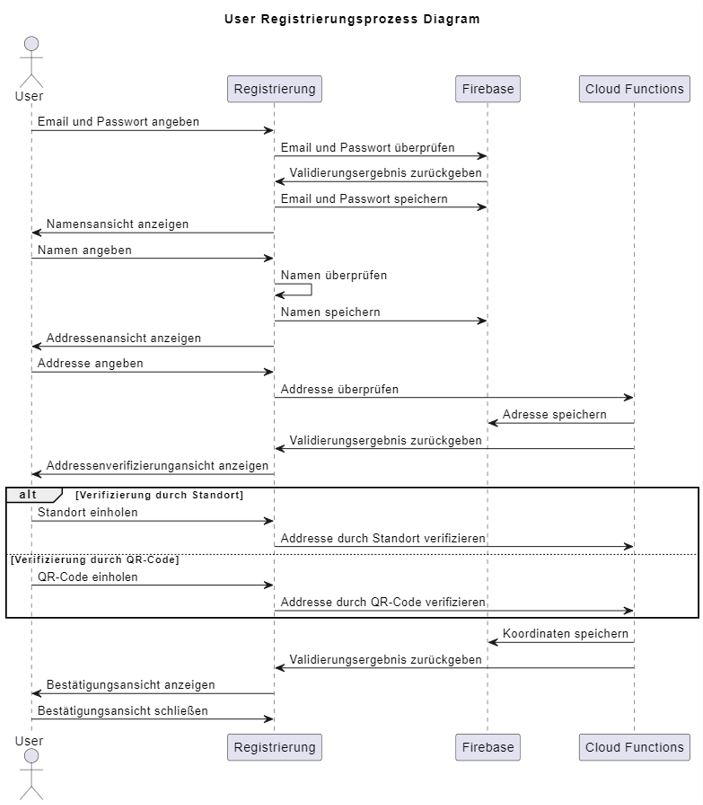
\includegraphics[width=\textwidth]{pics/registration-sequence.JPG}
  \caption{Registrierungsprozess}
\end{minipage}

\begin{figure}[h]
  \centering
  \begin{minipage}[b]{0.3\textwidth}
    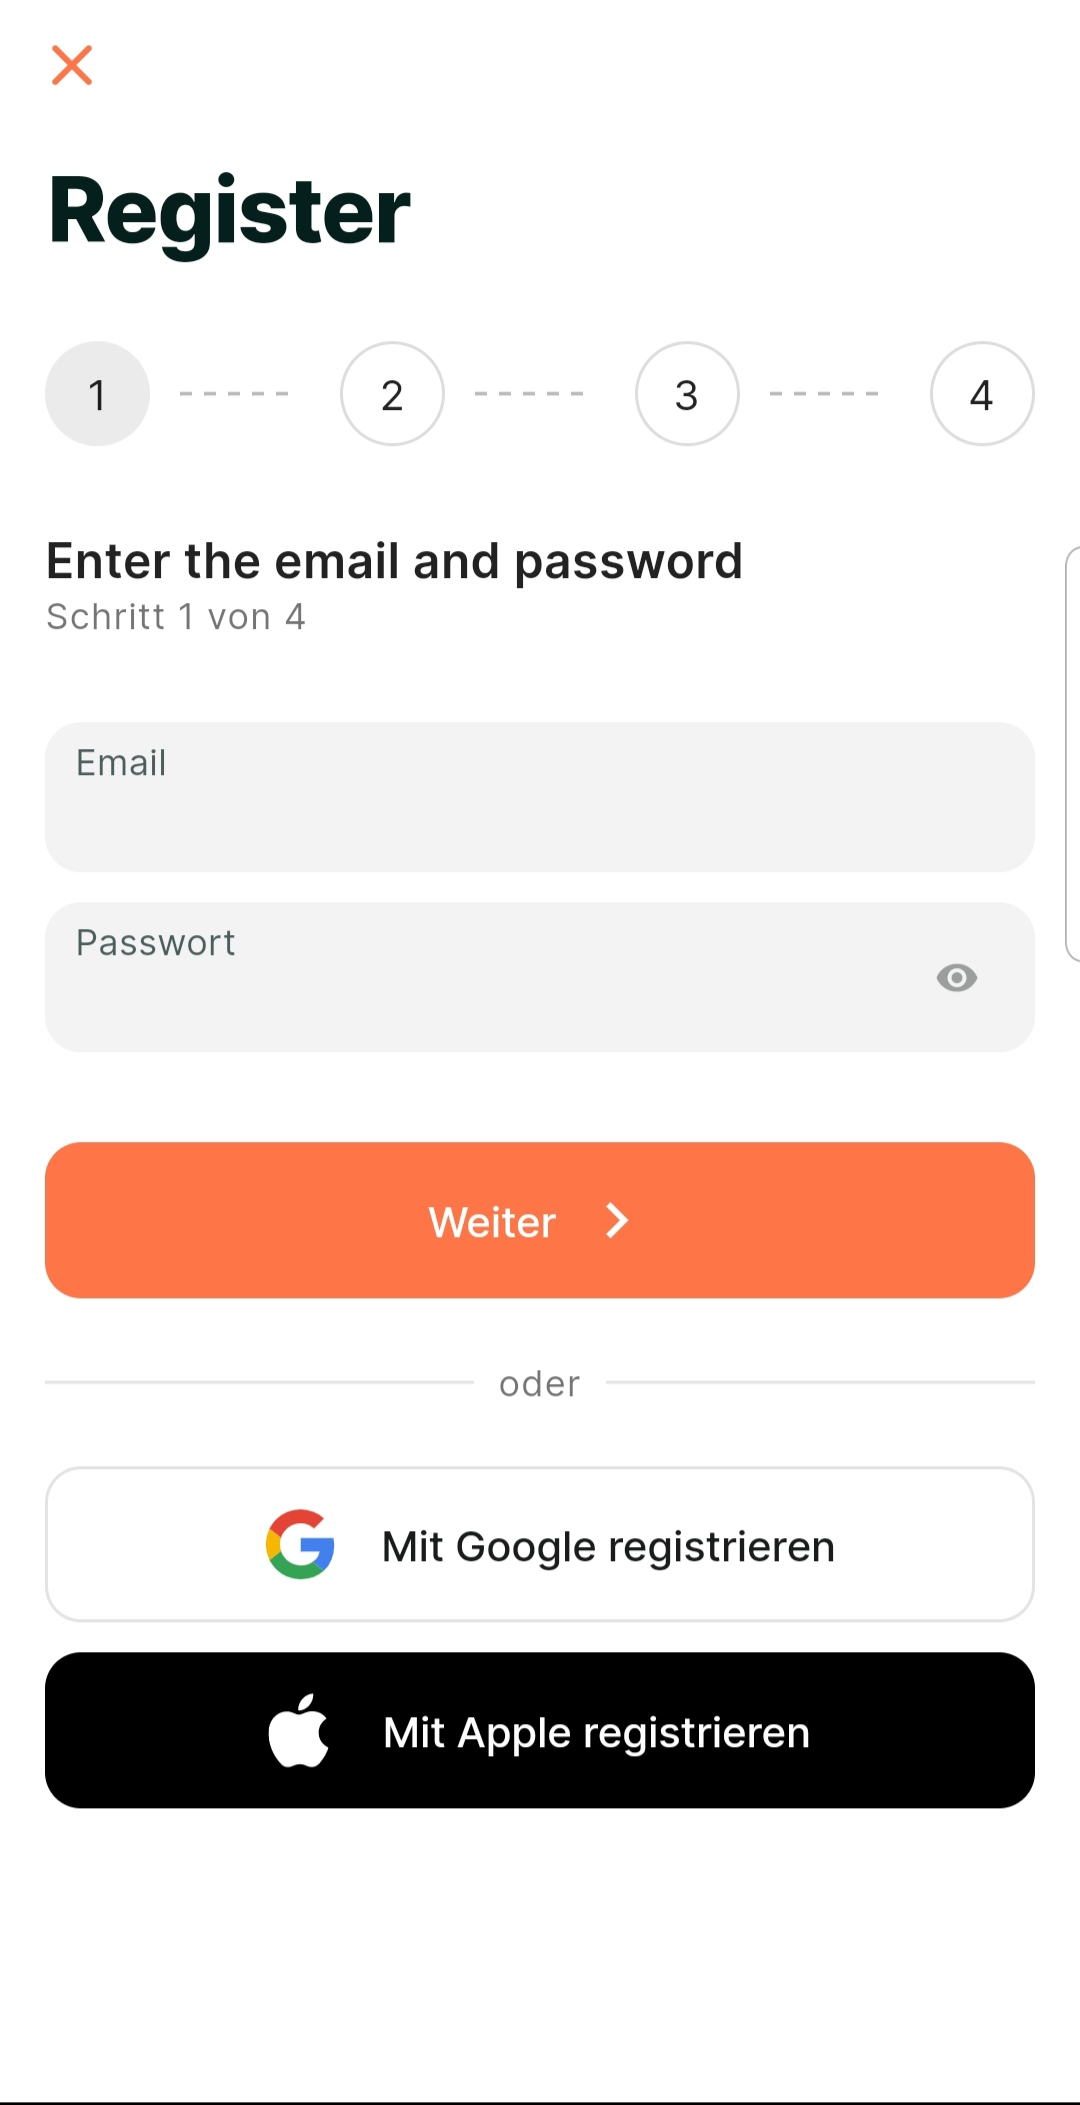
\includegraphics[width=\textwidth]{pics/registration-step-1.jpg}
    \caption{Email angeben}
  \end{minipage}
  \hfill
  \begin{minipage}[b]{0.3\textwidth}
    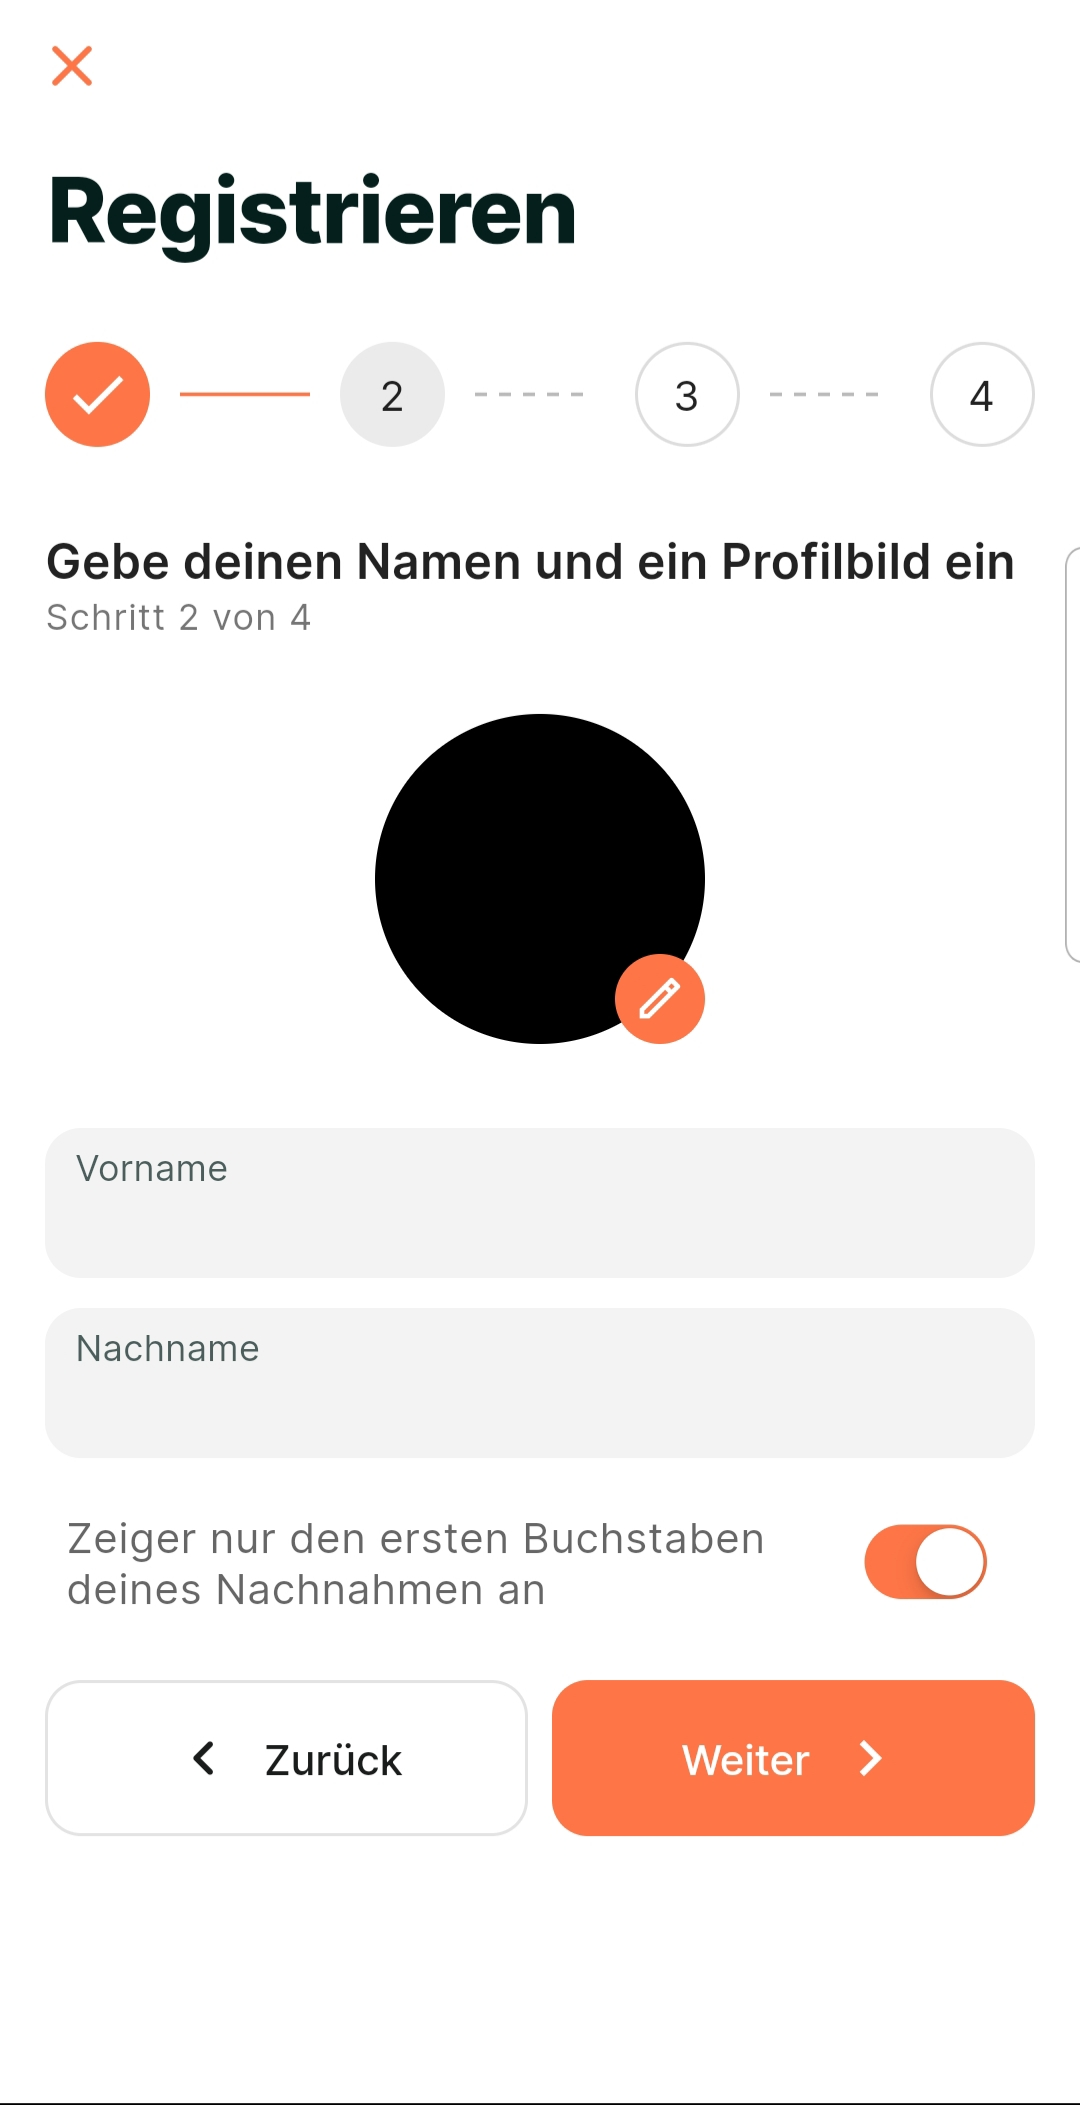
\includegraphics[width=\textwidth]{pics/registration-step-2.jpg}
    \caption{Namen angeben}
    \label{fig:post-more-menu}
  \end{minipage}
  \hfill
  \begin{minipage}[b]{0.3\textwidth}
    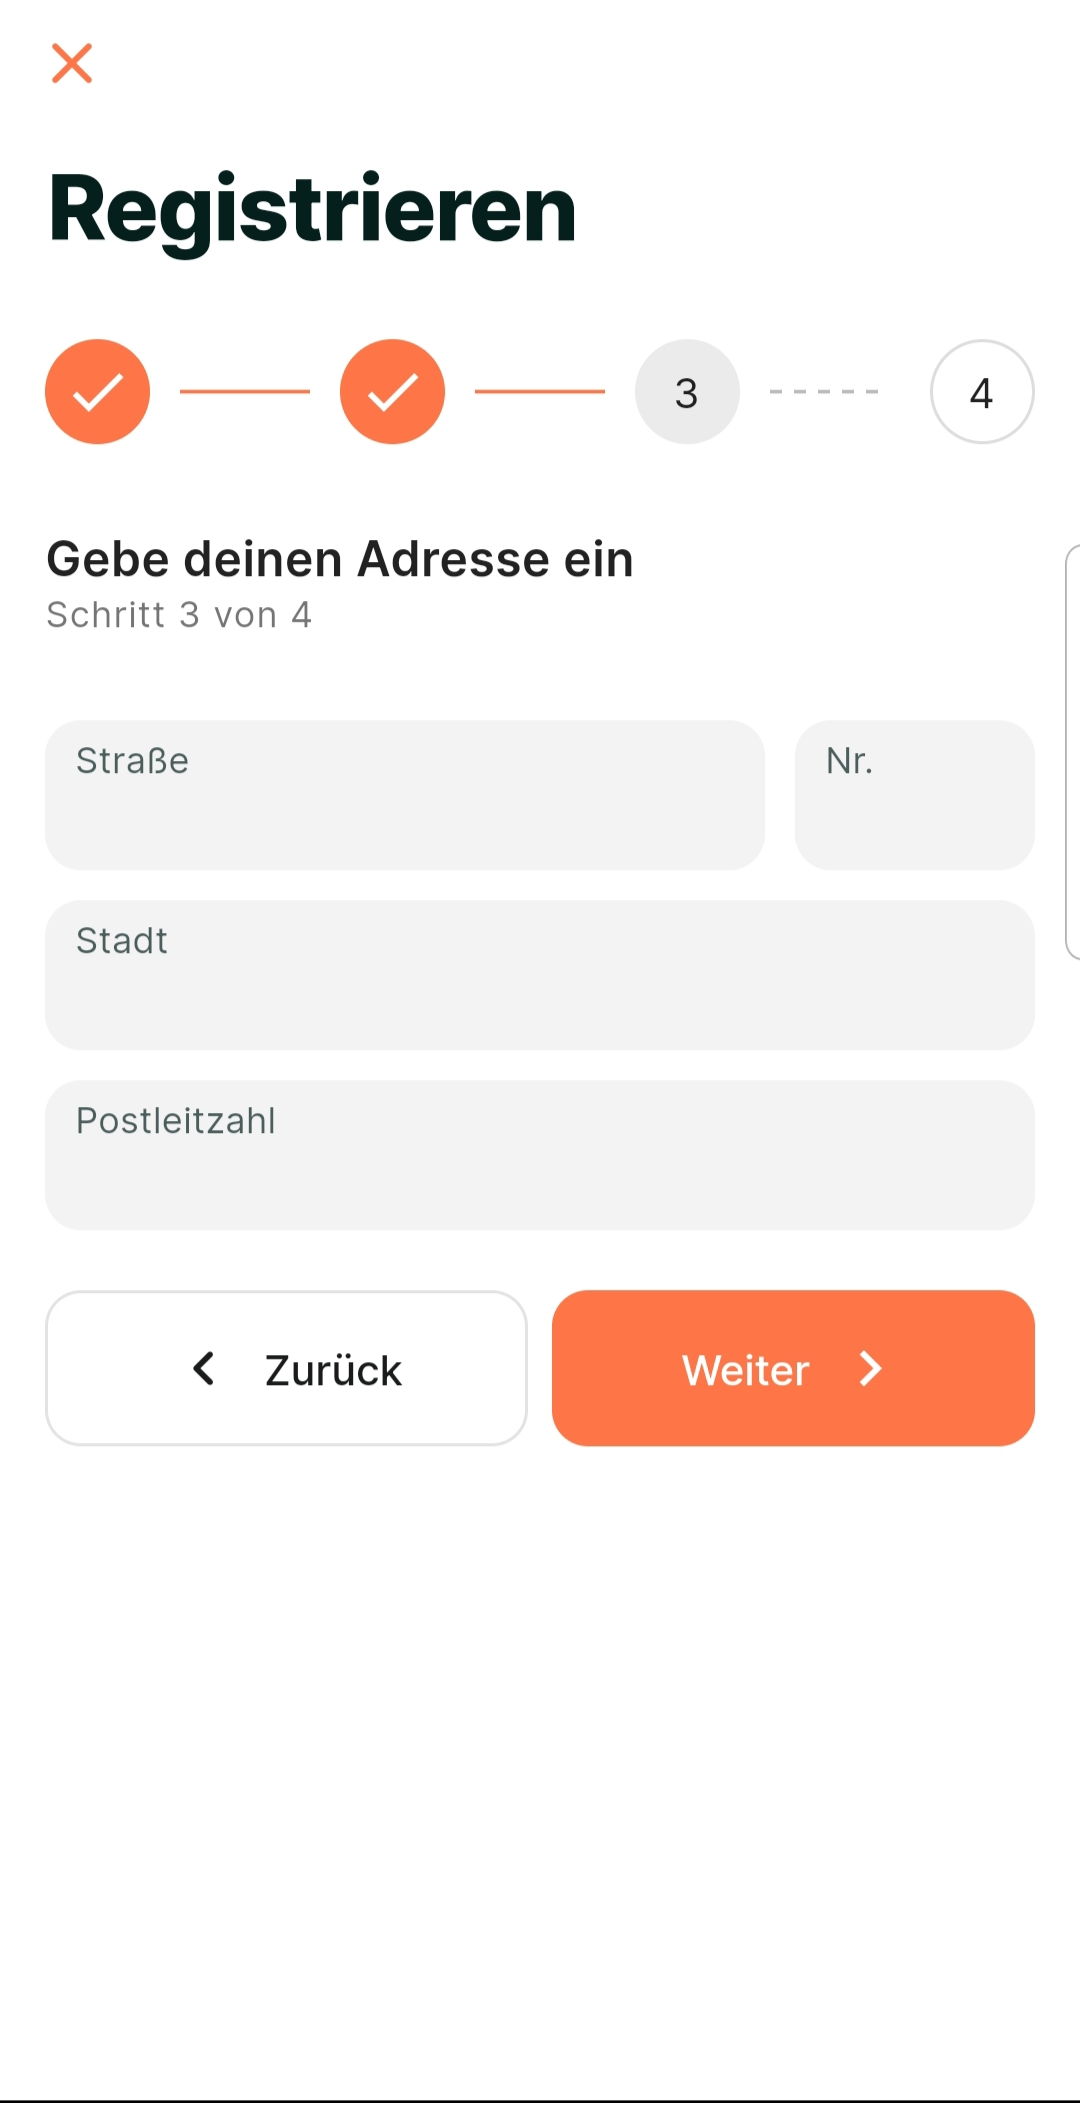
\includegraphics[width=\textwidth]{pics/registration-step-3.jpg}
    \caption{Addresse angeben}
    \label{fig:post-report-menu}
  \end{minipage}
  \hfill
  \begin{minipage}[b]{0.3\textwidth}
    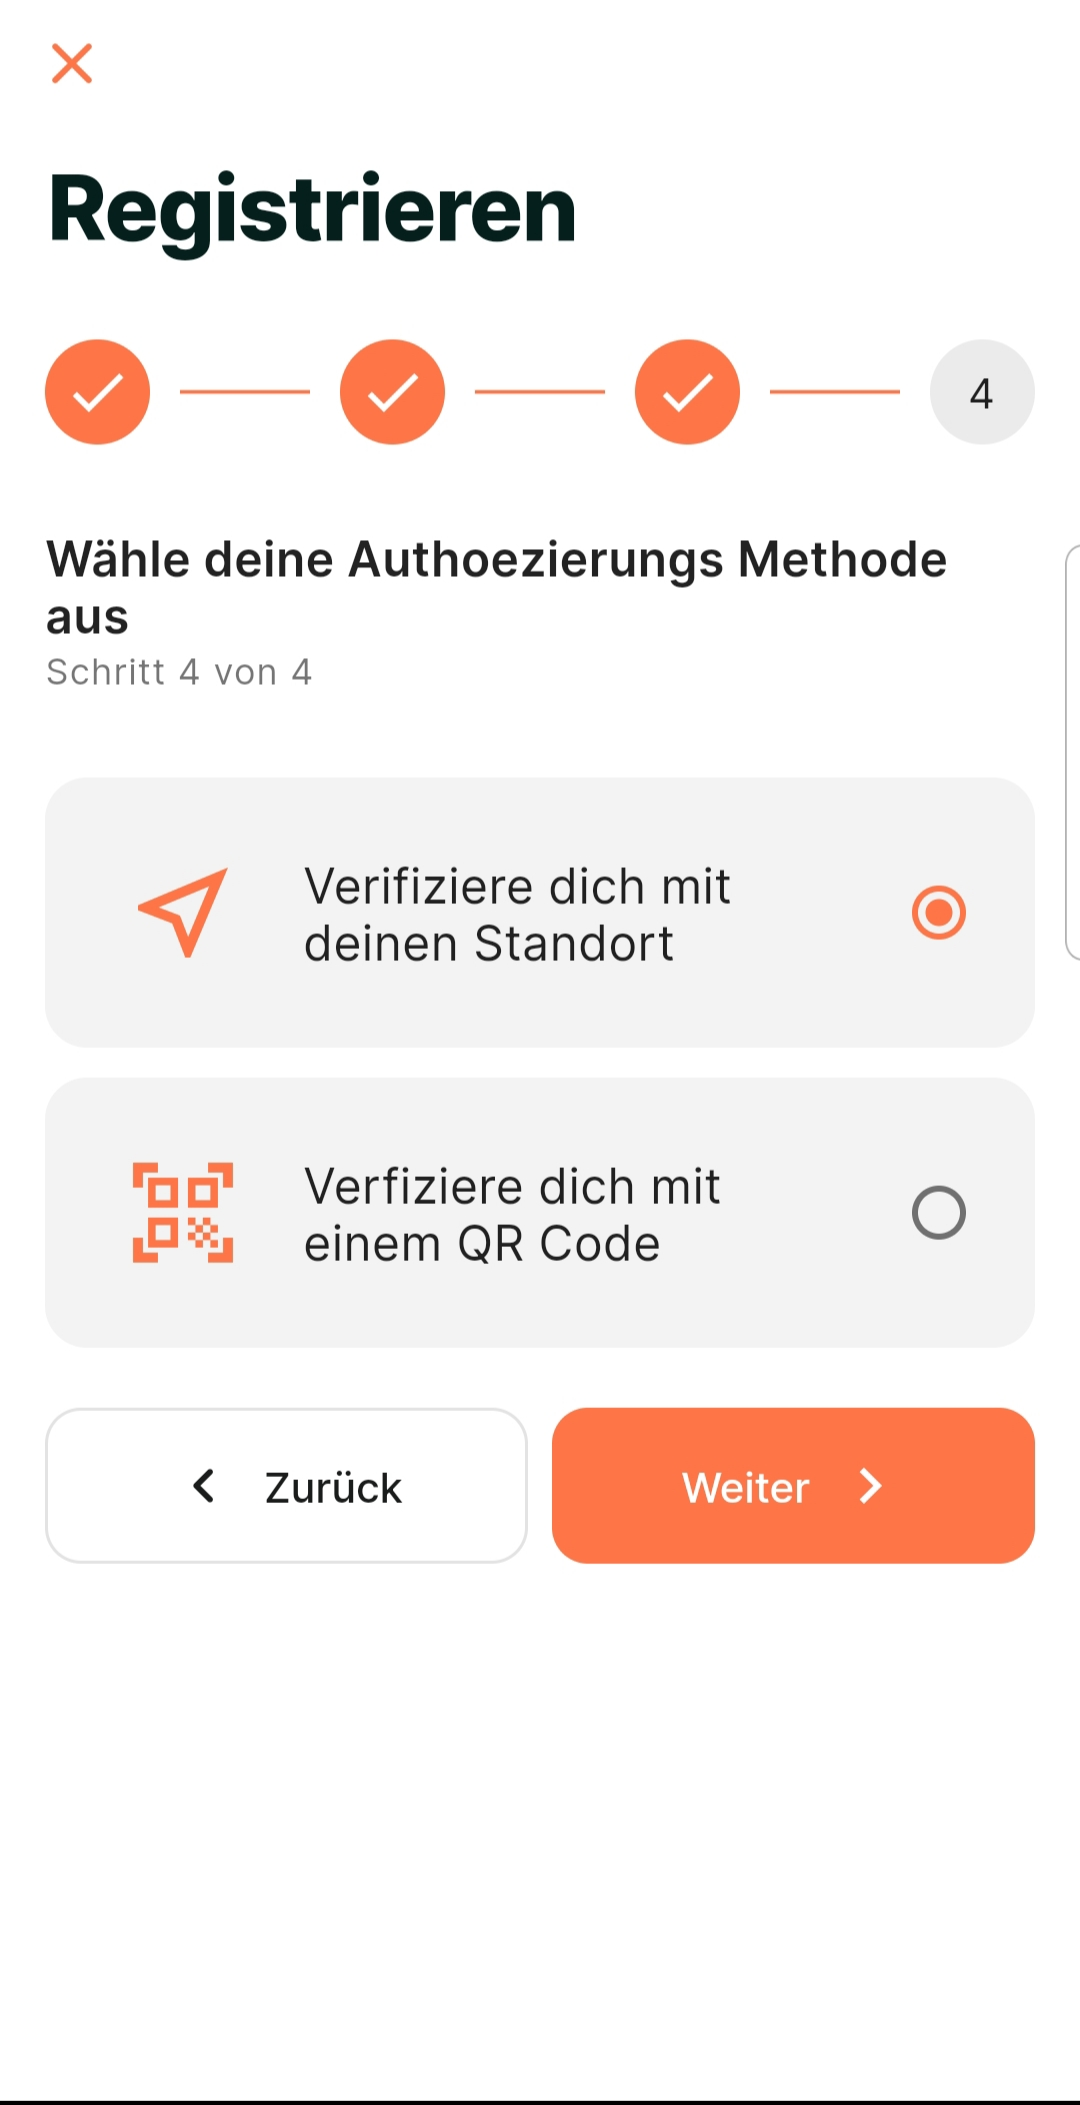
\includegraphics[width=\textwidth]{pics/registration-step-4.jpg}
    \caption{Addresse verifizieren}
    \label{fig:post-report-menu}
  \end{minipage}
  \hfill
  \begin{minipage}[b]{0.3\textwidth}
    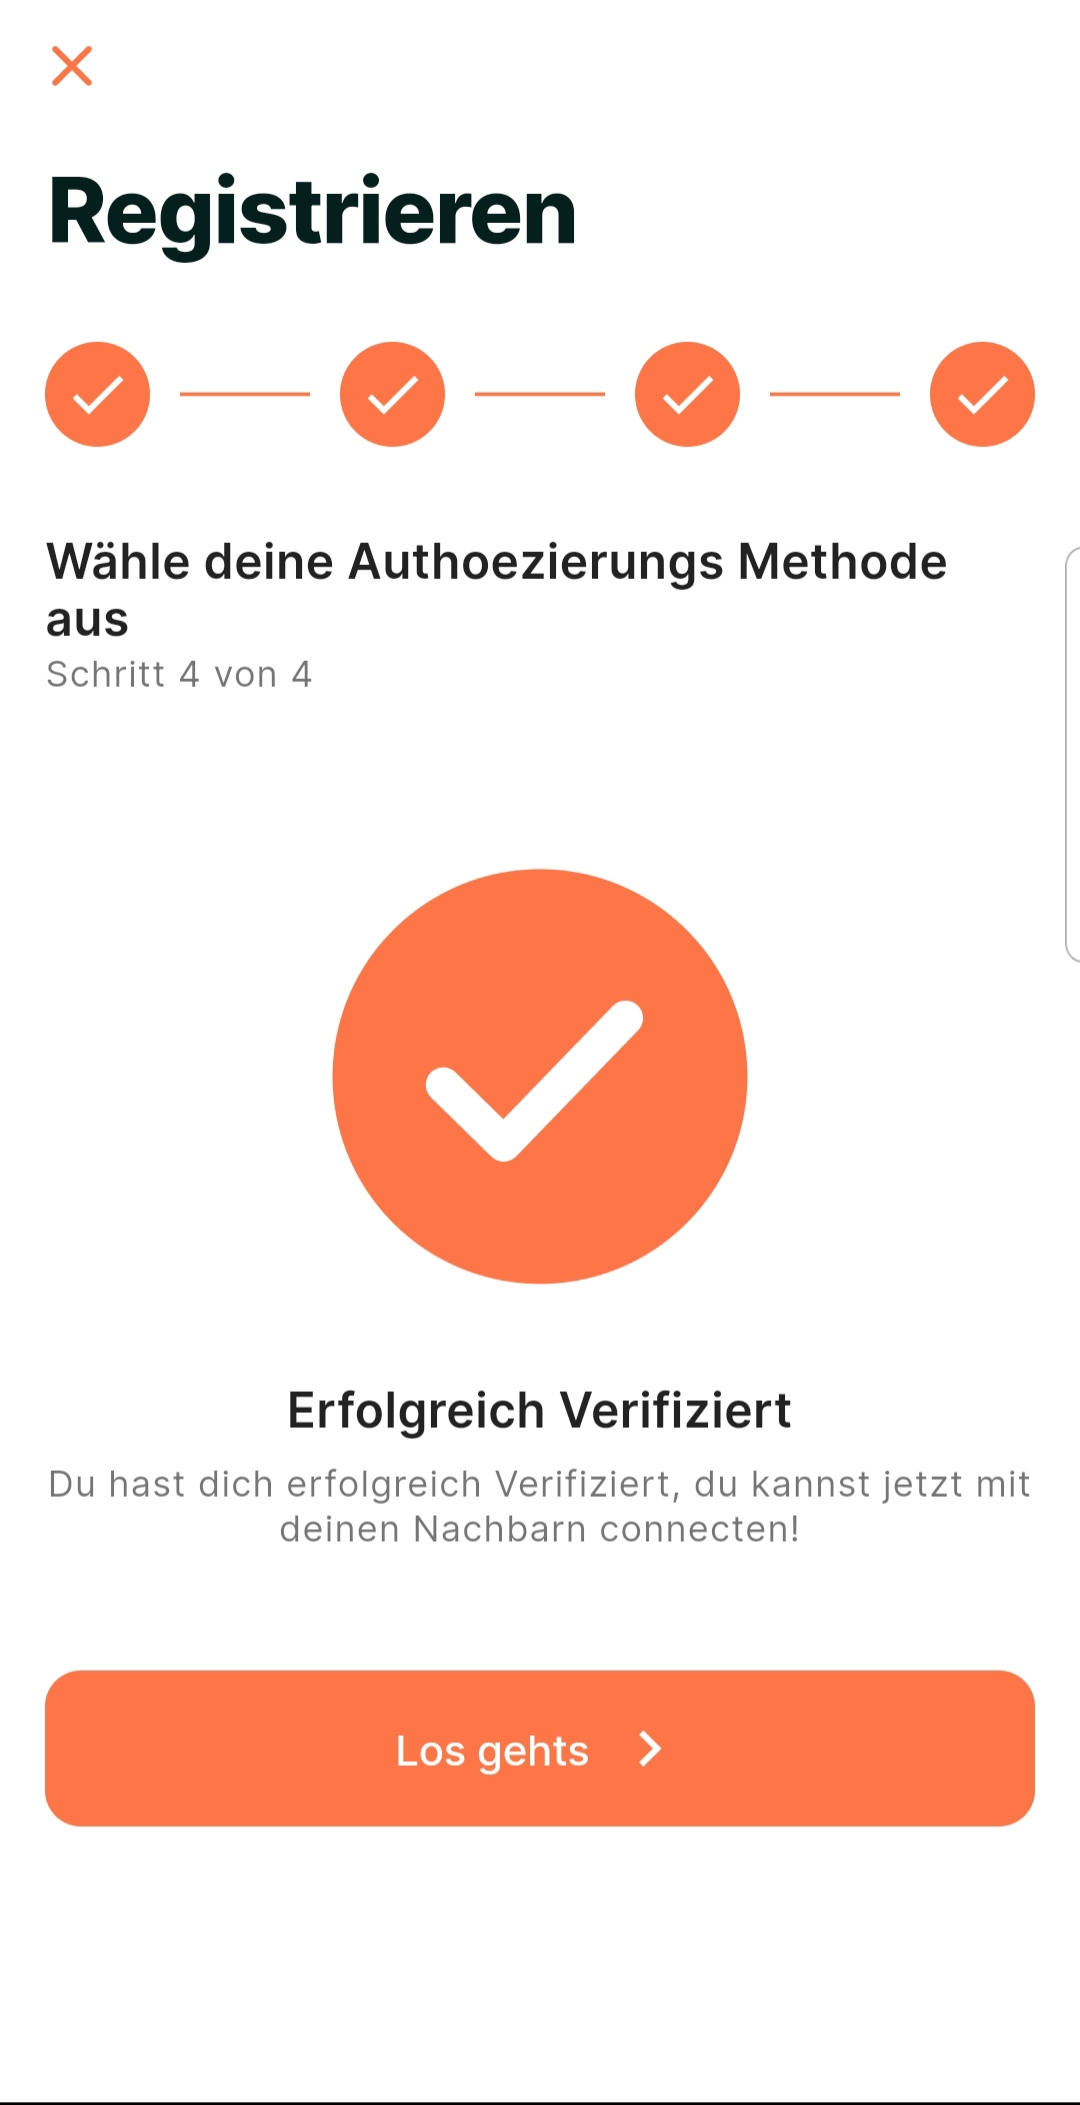
\includegraphics[width=\textwidth]{pics/registration-step-5.jpg}
    \caption{Registrierung abgeschlossen}
    \label{fig:post-report-menu}
  \end{minipage}
\end{figure}


\paragraph{Google Barcode-Scanning ML Kit}
\setauthor{Martin Hausleitner}
In Anbetracht der Entscheidung, Einladungscodes mithilfe von QR-Codes zu implementieren, ist es erforderlich, einen QR-Code-Scanner während des Registrierungsprozesses zu integrieren. Um eine zuverlässige Benutzererfahrung zu gewährleisten, wurde das Google Barcode-Scanning ML Kit als bevorzugte Technologie ausgewählt. In internen Tests zeigte sich, dass dieses Kit eine hohe Genauigkeit und Zuverlässigkeit aufweist.

Die Integration des Scanners wurde mithilfe des Pakets \href{https://pub.dev/packages/mobile_scanner}{mobile\_scanner} realisiert, welches auf der Plattform pub.dev verfügbar ist. Dieses Paket ermöglicht eine einfache Implementierung und Anpassung an die individuellen Anforderungen des Projekts. Die Verwendung des ML-Kits trägt dazu bei, die Leistungsfähigkeit der Anwendung zu verbessern und die Benutzerzufriedenheit zu erhöhen.


Diagram
erklärung
screenshots


\subsubsection{Firebase Authentifizierung}
\setauthor{Sandin Habibovic}

allg.


\subsection{Feed}
\setauthor{Sandin Habibovic}
Die Feed-Page ist die erste und wichtigste Anzeige auf der App. Hier werden alle aktuellen Beiträge und Updates von der Nachbarschaft angezeigt.

\subsection{Beiträge}
\setauthor{Sandin Habibovic}
Beiträge sind das Hauptkommunikationsmittel auf der App. Jedem Beitrag muss ein Titel, eine Beschreibung und eine Reichweite, unter der, der Beitrag sichtbar ist, angegeben werden. Weiters ist es möglich einem Beitrag ein Bild und Tags anzuhängen.

\subsubsection{Kategorien}
\setauthor{Sandin Habibovic}
Um Beiträge besser zuordnen zu können, muss der User den Beitrag vor dem Veröffentlichen in eine bestimmte Kategorie einteilen. Diese Kategorien ermöglichen es Usern, die Art Ihrer Anfrage ihm vorhinein besser zu spezifizieren und die Suche nach Beiträgen einer bestimmten Art zu vereinfachen. Bestimmte Kategorien werden weiters in Unterkategorien aufgeteilt, da diese ein zu weit gefächertes Genre an Anfragen umfassen.

Es existieren folgende Kategorien bzw. Unterkategorien:

\begin{compactitem}
  \item Mitteilung
  \begin{compactitem}
    \item Frage
    \item Appell
    \item Warnung
    \item Empfehlung
    \item Gefunden
  \end{compactitem}
  \item Suche
  \begin{compactitem}
    \item Hilfe
    \item Verloren
  \end{compactitem}
  \item Ausleihen
  \item Event
\end{compactitem}



Mitteilung:
Die Kategorie der Mitteilung dient dazu die Nachbarn über ein bestimmtes Ereignis oder Meldung zu informieren oder zu befragen.

Suche:
Die Kategorie der Suche dient dazu mit den Nachbarn im Falle einer Hilfesuche oder eines verloren gegangenen Objekts in Kontakt zu treten.

Ausleihen:
Die Kategorie des Ausleihens dient dazu die Nachbarn nach der Erlaubnis, sich ein bestimmtes Werkzeug oder Objekt ausborgen zu dürfen, zu bitten.

Event:
Die Kategorie des Events dient dazu die Nachbarn auf eine bestimmte Veranstaltung aufmerksam zu machen.


\subsubsection{Tags}
\setauthor{Sandin Habibovic}
Als Tag wird ein Schlüsselwort beschrieben, was man an ein Informationsgut anhängen kann, um es besser beschreiben zu können und/oder besser auffindbar zu machen. In der App werden Tags als eine Erweiterung der Kategorien verwendet, um es Usern zu ermöglichen Ihren Beitrag einem selbstdefinierten Typ zuzuordnen.

\subsubsection{Info}
\setauthor{Sandin Habibovic}
Jeder Beitrag hat eine eigene Sektion, wo wichtige Entscheidungsinformationen angegeben werden, wie der Stadtteil und die ungefähre Entfernung zum gegebenen Nachbarn und das Erstelldatum des Beitrags.

\subsubsection{Kommentare}
\setauthor{Sandin Habibovic}
Die Kommentarfunktion ermöglicht es den Usern unter einem Beitrag Ihre Meinung, Feedback oder sonstiges zu hinterlassen.

\subsubsection{Beitrag oder Kommentar Melden}
\setauthor{Sandin Habibovic}
Um auf unangebrachte Beiträge oder Kommentare schnell reagieren zu können, gibt es die Möglichkeit Beiträge oder Kommentare zu melden. Diese Meldungen werden auf Firestore gespeichert und können dann im Einzelnen überprüft werden. Fürs Melden muss ein Grund ausgewählt und eine genauere Beschreibung angegeben werden.
Gründe fürs Melden eines Beitrags oder Kommentars:

\begin{compactitem}
  \item Unangebrachter Inhalt
  \item Belästigung
  \item Betrug
  \item Spam
  \item Sonstiges


\end{compactitem}

\subsubsection{Autovervollständigung
  mit Künstliche Intelligenz}
\setauthor{Martin Hausleitner}
\paragraph{GPT-3.5-turbo}


\begin{figure}[H]
  \centering
  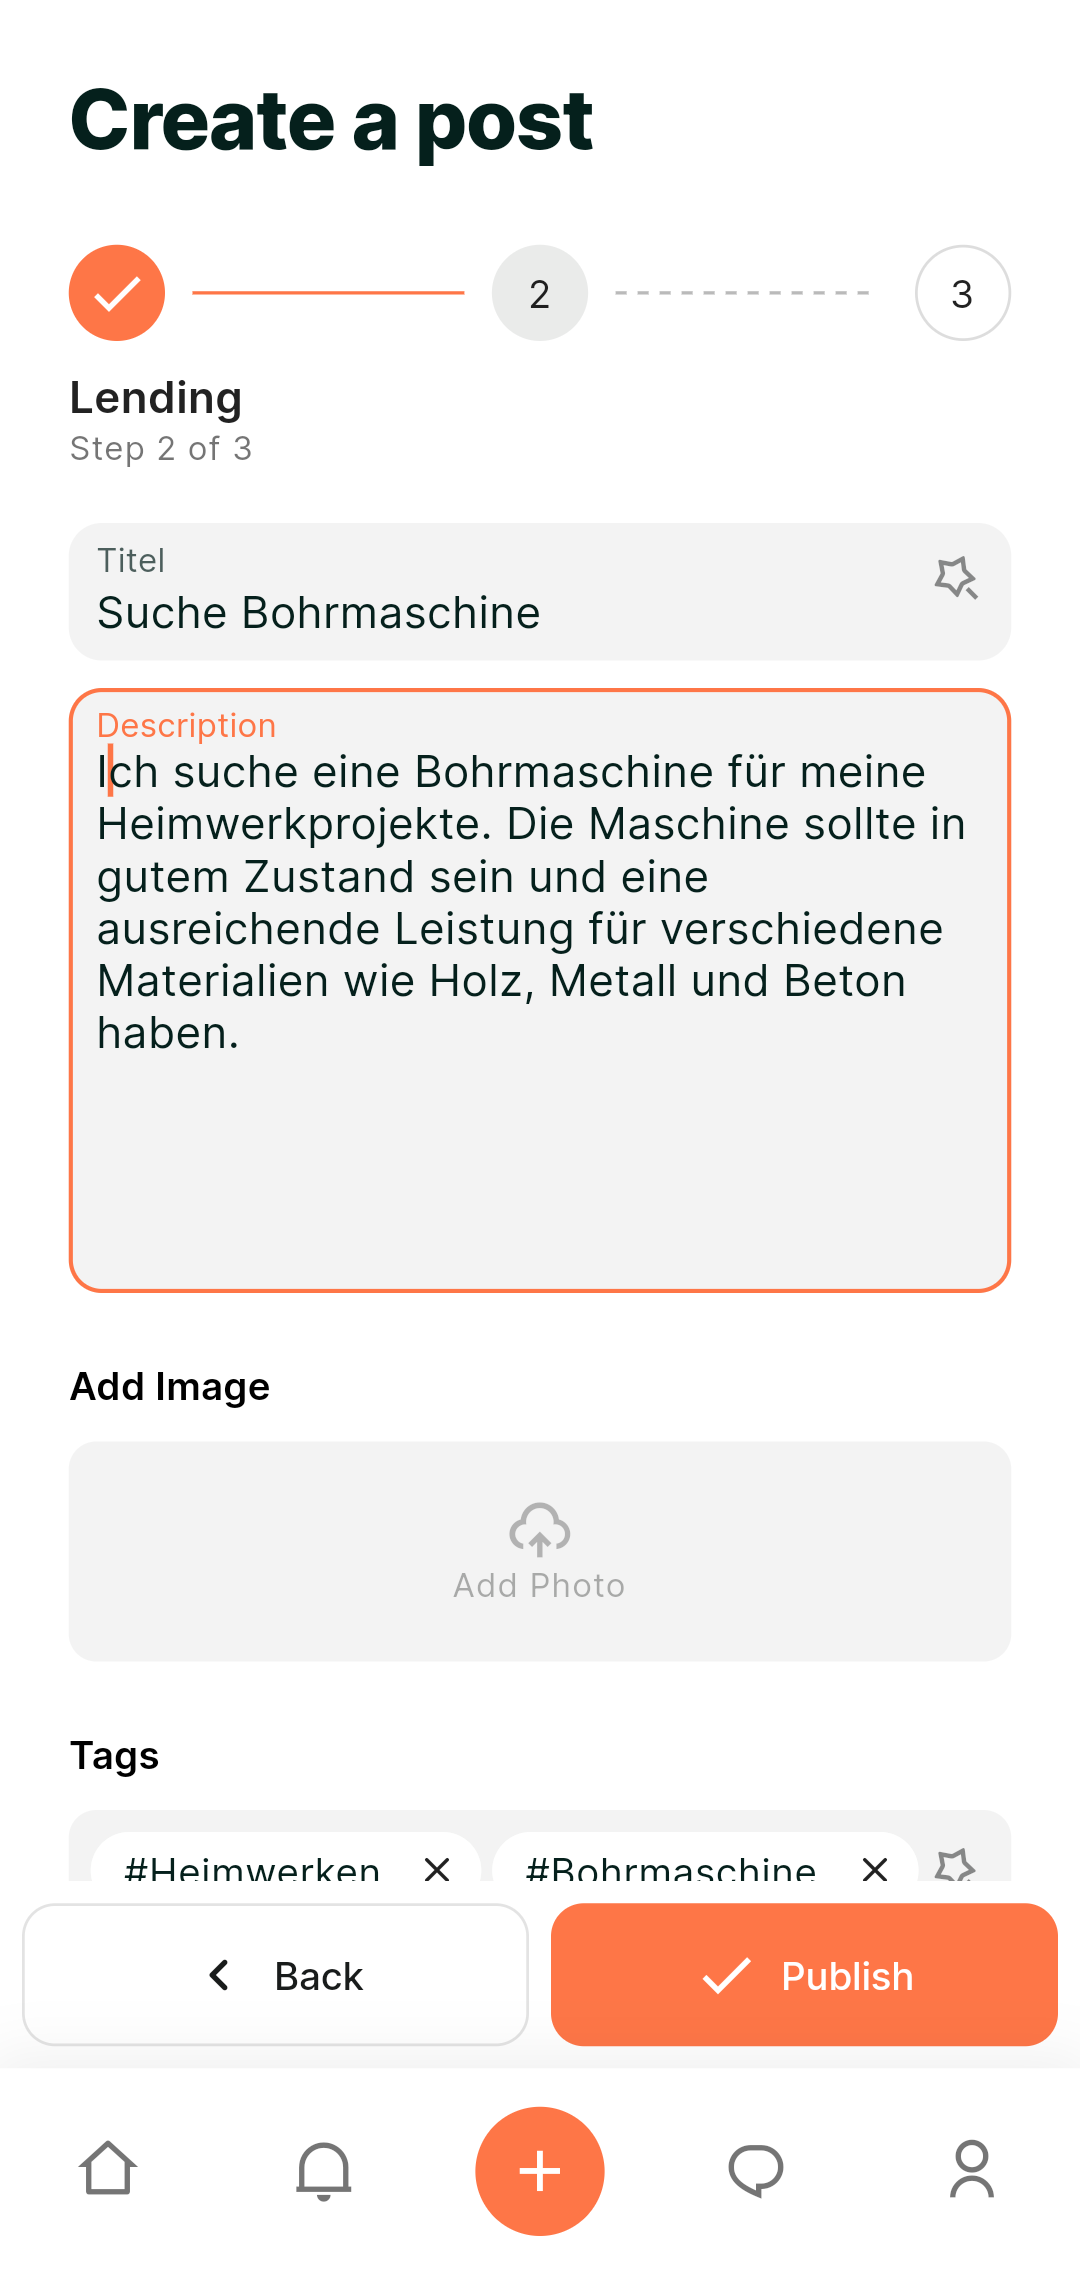
\includegraphics[width=0.3\textwidth]{pics/create-post.png}
  \caption{Schritt: 2 Beitrag erstellen}
  \label{fig:createpost}
\end{figure}


In jüngster Vergangenheit haben Fortschritte in der künstlichen Intelligenz (KI) dazu geführt, dass deren Implementierung in verschiedenen Produkten immer einfacher wird. Das Entwicklerteam hat daher beschlossen, auch in Nochba eine vereinfachte Implementierung durchzuführen. Mit der Veröffentlichung der GPT-3.5-turbo API von OpenAI wurde diese unmittelbar in Nochba integriert. Wie in der Abbildung \ref{fig:createpost} ersichtlich, befindet sich im Titelfeld ein Zauberstab-Symbol in der rechten oberen Ecke. Bei einem Klick darauf wird eine API-Anfrage an OpenAI gesendet. Um einen Titel basierend auf der Beschreibung zu erstellen, wird folgender Prompt benötigt:
\begin{verbatim}
beschreibung{ ${widget.descriptionController!.text} } passender Titel:
\end{verbatim}

Die KI liefert stets zuverlässig einen passenden Titel.

Ein ähnlicher Ansatz wurde auch für die Tags verfolgt. Der Titel und die Beschreibung wurden als Kontext für die KI verwendet. Nach mehreren Versuchen wurde der passende Prompt gefunden, da die KI-Ausgabe zunächst inkonsistent war und nicht erfolgreich in Tags umgewandelt werden konnte. Mit dem folgenden Prompt wurde der Output zuverlässiger:

\begin{verbatim}
titel{ $ {widget.titleController!.text }  } beschreibung { ${widget.descriptionController!.text }  } json hashtags richtige sprache: ["#
\end{verbatim}


Die letzten Zeichen ["\# wurden absichtlich gewählt, da die
KI-Ausgabe manchmal mit oder ohne \# geschrieben wurde, was
das Parsen der Tags erschwerte. Durch die Klammer und das \#
werden nun zuverlässig im JSON-Format und Tags mit \#
erstellt.

Der folgende Code \ref{lst:parseTags} wird verwendet, um die Tags aus der KI-Ausgabe zu parsen und sie anschließend dem TagsController zu übergeben:

\begin{lstlisting}[language=Java,caption=parseTags von 
  KI output,label=lst:parseTags]  
  
  List<String> parseTags(String chatOutput) {
    RegExp regExp = RegExp(r'(?<=#)[\p{Letter}]+', unicode: true);
    Iterable<RegExpMatch> matches = regExp.allMatches(chatOutput);
    List<String> tags = [];

    for (RegExpMatch match in matches) {
      String tag = match.group(0)!;
      tags.add(tag);
    }

    print(tags.toString());

    return tags;
  }
    
\end{lstlisting}




Da die Nutzung der KI kostenintensiv sein kann, wenn mehr Benutzer sie verwenden, ist die Nutzung auf maximal zwei Anfragen pro Benutzer für Titel- oder Tag-Generierung begrenzt. Zukünftig ist geplant, das System durch ein Nochba AI-Abo mit unbegrenzten Anfragen zu monetarisieren.

\subsubsection{Übersetzung mit Maschine Learning}

\paragraph{Google Translation ML Kit}

Für die Übersetzung von Beiträgen vom Deutschen ins Englische wurde eine kosteneffiziente Methode gesucht, um Kosten zu minimieren. Zunächst wurden bekannte Übersetzungs-APIs analysiert, aber dann stieß der Entwickler auf das Google ML Kit, welches 50 Sprachen übersetzen kann. Bemerkenswert ist, dass ein Sprachpaket etwa 5 MB umfasst und auch offline verwendet werden kann. Beim Start der App werden das deutsche und englische Sprachmodell heruntergeladen. Um einen Beitrag zu übersetzen, muss der Benutzer länger auf den Beitrag klicken, um die Übersetzung zu starten.



\paragraph{Google Language identification ML Kit}

Um eine Sprache überhaupt übersetzen zu können, benötigt man ein Werkzeug zur Spracherkennung. In dieser App wird das Google Spracherkennungs-ML-Kit verwendet. Bevor der Benutzer einen Beitrag übersetzen möchte, werden die Beschreibung und der Titel an das maschinelle Lernmodell gesendet, um die erkannte Sprache dem Übersetzungs-ML-Kit zu übergeben und eine Übersetzung durchzuführen.






\subsection{Filter}
\setauthor{Sandin Habibovic}
Der Filter bietet die Option die Beiträge nach bestimmten Kriterien zu filtern und die Suche nach bestimmten Beiträge zu vereinfachen. Der Filter unterteilt sich in einen Menüfilter und Hauptfilter.
Die Ansicht vom Menüfilter befindet sich direkt über den Beiträgen und ermöglicht eine schnelle Filterung nach einzig allein den Hauptkategorien.
Die Ansicht vom Hauptfilter taucht erst nach dem Antippen vom Filtersymbol auf und beinhaltet eine größere Auswahl an Filteroptionen. Darunter zählt neben dem Filtern nach Hauptkategorien auch die zusätzliche Möglichkeit genauer nach Unterkategorien zu suchen. Außerdem besteht auch die Option die Beiträge nach Datum oder Likes zu sortieren oder die Beiträge aufsteigend oder absteigend zu ordnen. Die wichtigste Filterkomponente ist der Range-Slider, womit die Beiträge nach der Reichweite gefiltert werden können, da die Entfernung zum Nachbarn eine der wichtigsten Entscheidungsfaktoren zum Antworten auf einem Beitrag ist.

\subsection{Suche}
\subsection{Typesense}
\subsection{Algolia}
diagram
\subsubsection{Firestore Sync}

\subsubsection{Algolia SDK}


\subsection{Chat}




\subsubsection{Google Smart Reply ML Kit}
\setauthor{Martin Hausleitner}
Die Implementierung des Google Smart Reply ML Kits wurde als sinnvolle Ergänzung in Betracht gezogen, um wiederkehrende und standardisierte Antworten in der Kommunikation zwischen Benutzern zu reduzieren. Ein Beispiel dafür ist die Nutzung solcher Plattformen wie Willhaben, bei denen häufig ähnliche Fragen und Antworten ausgetauscht werden.

\begin{figure}[H]
  \centering
  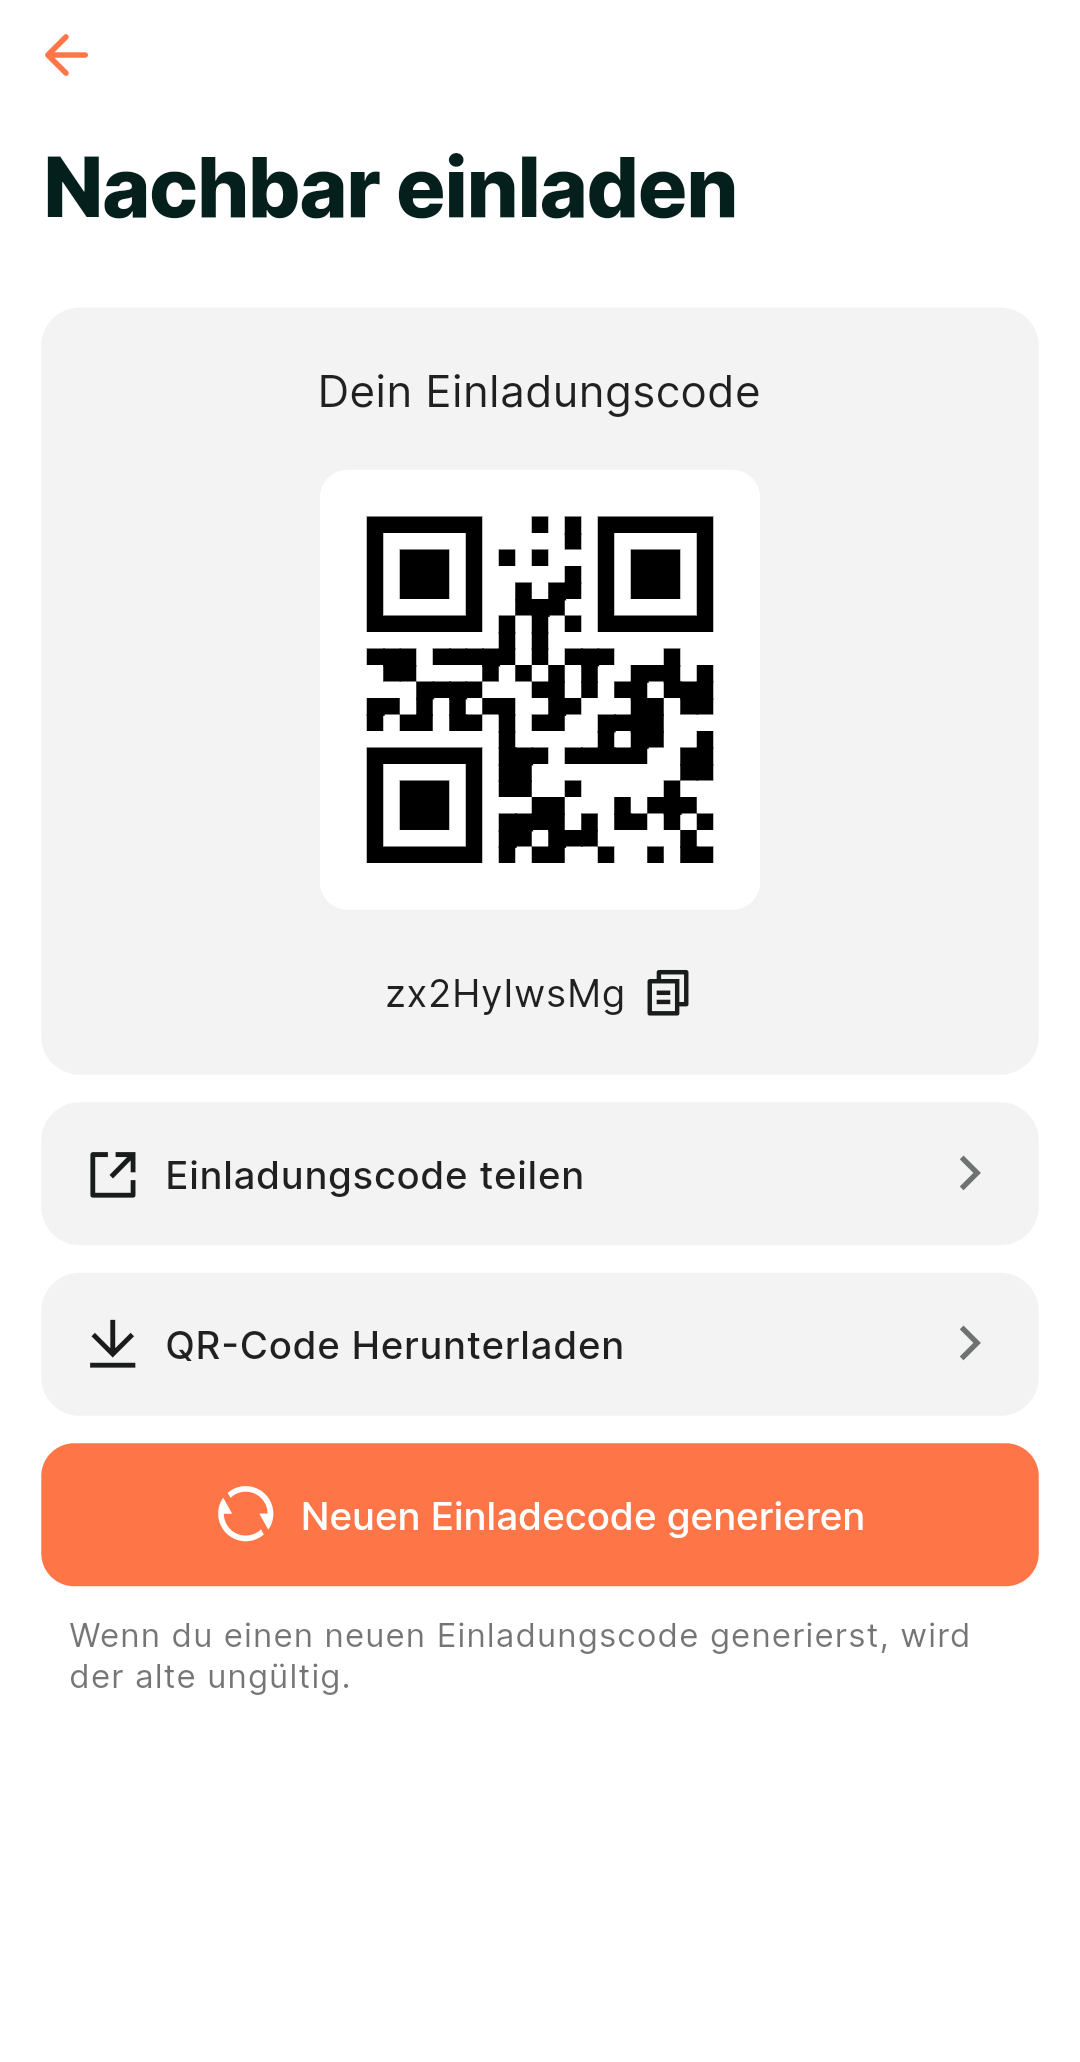
\includegraphics[width=0.3\textwidth]{pics/einladecode-page.png}
  \caption{Smart Replay im Chat}
  \label{fig:einladecode}
\end{figure}

Die Integration des Google Smart Reply ML Kits bietet den Benutzern verschiedene Antwortmöglichkeiten, die direkt über den Eingabefeld des Chats angezeigt werden. Dies ermöglicht eine effizientere und benutzerfreundlichere Kommunikation, da aufwendige manuelle Texteingaben vermieden werden können. Die Abbildung verdeutlicht, wie verschiedene Vorschläge im Eingabefeld angezeigt werden.

Das Google Smart Reply System nutzt die letzten zehn Nachrichten als Kontext, um adäquate und relevante Antwortvorschläge zu generieren. Die Anwendung von maschinellem Lernen in diesem Kontext trägt zur Verbesserung der Benutzererfahrung bei und ermöglicht eine effizientere Kommunikation. Auf diese Weise können die Benutzer schnell und einfach auf eingehende Nachrichten reagieren, wodurch wertvolle Zeit gespart und mögliche Frustrationen vermieden werden.

\subsubsection{Flyer Package}

\subsection{Profil}
\setauthor{Sandin Habibovic}
Die Profilanzeige ist die öffentliche Informationsstelle über den User. In dieser Anzeige werden als erster Eindruck der Name und das Profilbild vom User angezeigt. Genauere Informationen über den User können im Bereich Nutzerinfo gefunden werden. Darunter zählen:
\begin{compactitem}
  \item Geburtstag
  \item Beruf
  \item Bio
\end{compactitem}
Außerdem beinhaltet die Anzeige eine eigene Beitragssicht, wo alle Beiträge vom jeweiligen User eingesehen werden können.

\subsubsection{Profil Melden}
\setauthor{Sandin Habibovic}
Falls das Profil vom User unangebrachten Inhalt aufweist, besteht die Möglichkeit das Profil zu melden.

\subsection{Benachrichtigungen}
\setauthor{Sandin Habibovic}
Benachrichtigungen dienen dazu die Nachbarn über mögliche
Hilfsbereitstellungen zu informieren, bevor der Kontakt
überhaupt entsteht. Die Benachrichtigung zeigt den Nachbarn
an, der in Kontakt treten möchte, und möglicherweise den
Beitrag auf dem geantwortet wurde. Außerdem ist die
Benachrichtigung mit einem „Annehmen“- und „Ablehnen“-
Button ausgestattet, womit das Hilfsangebot angenommen oder
abgelehnt werden kann.

\subsection{Einladecode}
\setauthor{Martin Hausleitner}

\begin{figure}[H]
  \centering
  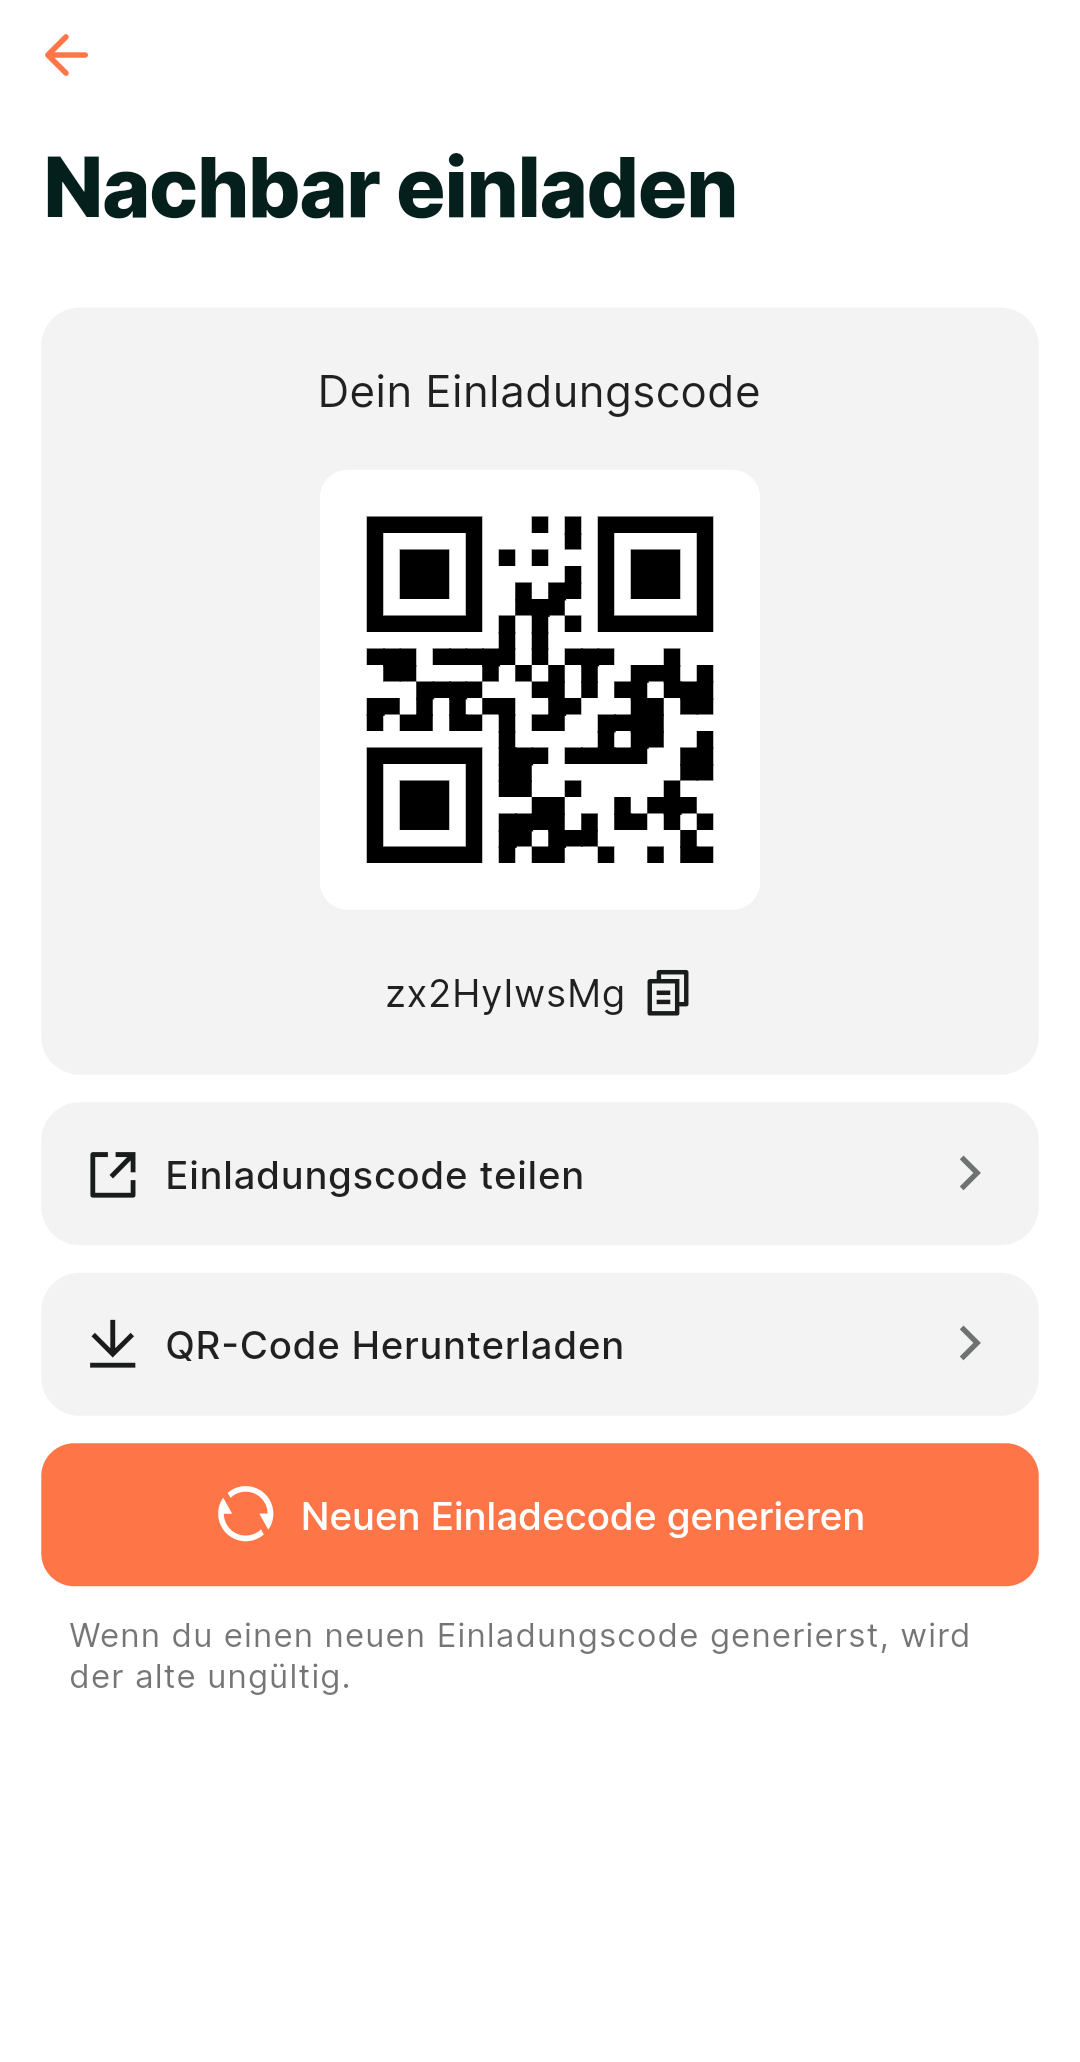
\includegraphics[width=0.3\textwidth]{pics/einladecode-page.png}
  \caption{Einladecode-Seite in der App}
  \label{fig:einladecode}
\end{figure}
Eine der beiden Verifizierungsmethoden basiert auf der Nutzung von Einladungscodes. Als Inspiration diente die deutsche App "Nebenan", die ebenfalls eine Verifizierung über einen Code ermöglicht. Da das Team dies als gute Lösung erachtete, wurde ein ähnlicher Ansatz übernommen.

Jeder Code hat eine Reichweite von 1 km, ausgehend von der Adresse des Benutzers, der den Code generiert. Dies soll verhindern, dass ein Code missbräuchlich verwendet wird. Der Aktionsradius, in dem der Benutzer den Code nutzen kann, kann von den Administratoren variabel eingestellt werden.

Zudem wird für die Entwickler protokolliert, wer welchen
Code zur Verifizierung verwendet hat, um im Falle eines
Missbrauchs entsprechende Maßnahmen ergreifen zu können, wie
beispielsweise das Sperren des Codes. Administratoren haben
ebenfalls die Möglichkeit, Codes zu deaktivieren.
\subsubsection{Einladungsmöglichkeiten}
\setauthor{Martin Hausleitner}


Folgende Punkte sinder in der Abbildung
\ref{fig:einladecode} zu erkennen.


\begin{enumerate}[label=\arabic*.]
  \item \textbf{Generierung eines QR-Codes:}
        \begin{itemize}
          \item Beim Öffnen der Seite "Nachbar einladen" wird automatisch ein QR-Code generiert.
          \item Nutzer können den generierten Code in die Zwischenablage kopieren, indem sie den Button neben dem Code betätigen.
        \end{itemize}

  \item \textbf{Teilen des Einladungscodes:}
        \begin{itemize}
          \item Bei dem Button "Einladungscode teilen" wird eine Nachricht mit dem generierten Code erstellt.
          \item Der Nutzer kann die Nachricht mithilfe des systemspezifischen Sharesheets teilen.
        \end{itemize}

  \item \textbf{Herunterladen des QR-Codes:}
        \begin{itemize}
          \item Unter "QR-Code herunterladen" wird eine PNG-Datei des Einladungs-QR-Codes erstellt.
          \item Die Datei wird im systemspezifischen Sharesheet geöffnet, um sie speichern zu können.
        \end{itemize}

  \item \textbf{Generierung eines neuen Einladungscodes:}
        \begin{itemize}
          \item Der orangefarbene Button "Neuen Einladungscode generieren" ermöglicht das Erstellen eines neuen Codes.
          \item Sobald der Nutzer einen neuen Code erstellt, wird der vorherige Code deaktiviert.
        \end{itemize}
\end{enumerate}

Verifizierte Nutzer können alle 24 Stunden einen
Einladungscode generieren.

Die Verifizierung erfolgt, indem der Benutzer bei der Registrierung die Option "Mit Einladungscode verifizieren" auswählt. Anschließend hat er die Möglichkeit, den Einladungscode entweder über den integrierten QR-Code-Scanner zu scannen oder manuell einzugeben. Für die Implementierung des QR-Code-Scanners wurde das Flutter-Paket \href{https://pub.dev/packages/mobile_scanner}{mobile\_scanner} verwendet, welches auf Googles MLKit \cite{googlemlkit} basiert. MLKit ist eine Machine-Learning-Bibliothek, die im vorliegenden Fall für das zuverlässige und schnelle Scannen von QR-Codes eingesetzt wird. Diese Bibliothek ermöglicht es, komplexe Funktionen wie das Erkennen von QR-Codes effizient und präzise zu implementieren. Der einzige Nachteil dieses Pakets ist der hohe Speicherbedarf von etwa 10 MB. Daher ist in Zukunft geplant, das MLKit nur bei Bedarf herunterzuladen und nach erfolgreicher Verifizierung des Benutzers wieder zu entfernen.

Der gescannte oder eingegebene Code wird anschließend an die Cloud-Funktion \texttt{checkVerificationCode} (siehe Abschnitt \ref{subsec:registrierung-verify}) gesendet und überprüft, ob der Code korrekt ist.



\subsection{Einstellungen}
\setauthor{Sandin Habibovic}
Die Einstellungssicht der Anwendung bietet eine Reihe an nützlichen Funktionen, die dem User mehr Kontrolle über sein Konto geben.
Dazu gehört zu einem die Option, die Sprache der App umzustellen, um dem User zu ermöglichen, die Anwendung in der bevorzugten Sprache zu nutzen. Zum derzeitigen Stand kann die App sich in zwei Sprachen übersetzen lassen: Deutsch und Englisch.
Darüber hinaus können Benutzer auch entscheiden, ob sie Benachrichtigungen erhalten möchten oder nicht, und diese Einstellungen jederzeit ein- oder ausschalten. Diese Einstellungen bieten den Benutzern eine höhere Privatsphäre und Personalisierungsmöglichkeiten, um die Anwendung besser an ihre individuellen Bedürfnisse anzupassen.
Zu den weiteren Einstellungen gehört das Umändern der E-Mail oder des Passworts, um die Sicherheit des Kontos zu gewährleisten und unbefugten Zugriff zu verhindern.
Die letzte Funktion in der Einstellungssicht ist das Löschen des eigenen Kontos, womit alle Daten des Users gelöscht werden. Vor dem endgültigen Löschen des Kontos wird der User allerdings aufgefordert, seine Entscheidung zu bestätigen.

\subsection{Feedback}
\setauthor{Martin Hausleitner}
Während der Testphase besteht das Ziel darin, eine effiziente Methode zur Sammlung von Feedback zu finden. Für ein detailliertes Verständnis von Fehlermeldungen ist die Bereitstellung von Screenshots äußerst hilfreich. Aus diesem Grund wurden Packages untersucht, die das Erstellen von Screenshots ermöglichen und zusätzliche Informationen als Kontext hinzufügen können. Das ausgewählte Package ist \href{https://pub.dev/packages/feedback}{feedback}. Dieses erlaubt es den Nutzern, Screenshots anzufertigen, Annotationen hinzuzufügen und anschließend einen entsprechenden Textkontext einzufügen. Eine nützliche Funktion ermöglicht es den Nutzern, bei Bedarf erneut zu navigieren und den Screenshot zu wiederholen.

Um den Feedback-View zu initiieren, wurde das Package \href{https://pub.dev/packages/shake}{shake} verwendet. Dieses wird durch eine bestimmte Bewegung des Mobilgeräts aktiviert. Bei der Implementierung dieser Funktion wurden ähnliche Mechanismen berücksichtigt, die in anderen Anwendungen zur Feedback-Erhebung verwendet werden.

Das von uns gewählte Vorgehen zur Analyse des Feedbacks erfolgt über die Trello-API, welche es uns ermöglicht, ein entsprechendes Dashboard zur Erfassung und Bearbeitung der Meldungen zu erstellen. Die erfassten Informationen, wie beispielsweise der Screenshot, der Text, das Datum und relevante Systeminformationen, dienen uns als Grundlage für eine weitere Auswertung und Fehlerbehebung. Trello erleichtert uns die Verwaltung des Feedbacks auf kostenlose Weise und stellt somit ein adäquates Instrument zur Unterstützung des Entwicklungsprozesses dar.


\section{UI/UX Design}
Das Design der Nachbarschafts-App war für das Team von hoher Bedeutung, weshalb der Designer Martin Hausleitner erheblichen Zeit- und Arbeitsaufwand aufwendete, um ein anspruchsvolles Design zu gestalten. Angesichts der Tatsache, dass die App ein breites Publikum ansprechen soll, einschließlich verschiedener Altersgruppen, war es von entscheidender Bedeutung sicherzustellen, dass die Benutzer die App einfach und intuitiv bedienen können. Um dieses Ziel zu erreichen, wurde eine klare Struktur und Navigation in das Design integriert, um den Benutzern eine einfache und effektive Nutzung der gewünschten Funktionen zu ermöglichen. Es wurde darauf geachtet, dass die Buttons gut erkennbar und mit aussagekräftigen Icons und verständlichen Beschriftungen versehen sind, um Verwirrung zu vermeiden. Weiterhin wurde das Design der Karten auf eine organische Weise gestaltet, um ein harmonisches und ästhetisches Gesamtbild zu erzeugen.
\setauthor{Martin Hausleitner}
\subsection{Inspiration}
Während des Designprozesses für die App wurden umfangreiche Recherchen im Bereich App-Design durchgeführt. Das Ziel war, die App so intuitiv wie möglich zu gestalten, um eine benutzerfreundliche Erfahrung sicherzustellen. Dabei wurden bekannte Social-Media-Apps wie \href{https://twitter.com/}{Twitter}, \href{https://www.instagram.com/}{Instagram} und \href{https://www.tiktok.com/}{TikTok} als Orientierung genutzt, da diese bereits erfolgreich auf dem Markt etabliert sind und von vielen Menschen vertraut genutzt werden.

Zusätzlich diente die erfolgreichste Nachbarschafts-App in Deutschland, \href{https://nebenan.de/}{Nebenan}, als Grundlage für die App-Entwicklung. Allerdings wurde festgestellt, dass ihre App sehr kompliziert aufgebaut und unübersichtlich ist. Daher wurde dies als Chance gesehen, um es besser zu machen.

Zur Entwicklung eines einfachen und schlichten Designs wurden Inspirationen von Websites wie \href{https://dribbble.com/}{Dribble} und \href{https://mobbin.design/}{Mobbin} genutzt. Insgesamt war die Recherche und Inspiration für das Design der App ein wichtiger Schritt, um sicherzustellen, dass Benutzer eine ansprechende und intuitive Erfahrung haben.

\subsection{Prototyping}
Das Team legte von Anfang an großen Wert auf eine exzellente
Benutzererfahrung, und daher war es ihnen klar, dass ein
Prototyp gestaltet werden musste. Das Prototyping hatte für
die Entwickler den großen Vorteil, dass sie beim
Programmieren in Flutter nicht mehr lange darüber nachdenken
mussten, wie Menüs oder Bildschirme gestaltet werden
sollten. Somit war es einfach für Teammitglieder, die nicht
mit Design vertraut waren, den Prototypen als Grundlage zu
nutzen, um ihre Umsetzung in Flutter zu gestalten. Der
Prototyp selbst war für den Designer Martin Hausleitner eine
Reise durch verschiedene Designer-Tools, die im folgenden
Absatz genauer behandelt werden.


\subsubsection{Framer}

Framer ist eine Software, die es Benutzern ermöglicht, schnell und einfach ansprechende Prototypen von mobilen Anwendungen und Websites zu erstellen. Das Tool wurde ursprünglich als Prototyping-Tool für Designer entwickelt, um Designs schnell zu testen und zu verfeinern, bevor sie in die Entwicklung übergehen.

Erfolgreiche Apps wie Spotify haben Framer im Rahmen ihres
Prototyping-Prozesses verwendet, um schnell und effizient
funktionierende App-Designs zu erstellen. Framer ist eine
schnelle und effiziente Möglichkeit, um Ideen in die Tat
umzusetzen, ohne sich durch langwierige Entwicklungsprozesse
zu quälen. Dies sind überzeugende Gründe für den Designer, den ersten Prototypen mit Framer zu gestalten.

\begin{figure}[h]
  \centering
  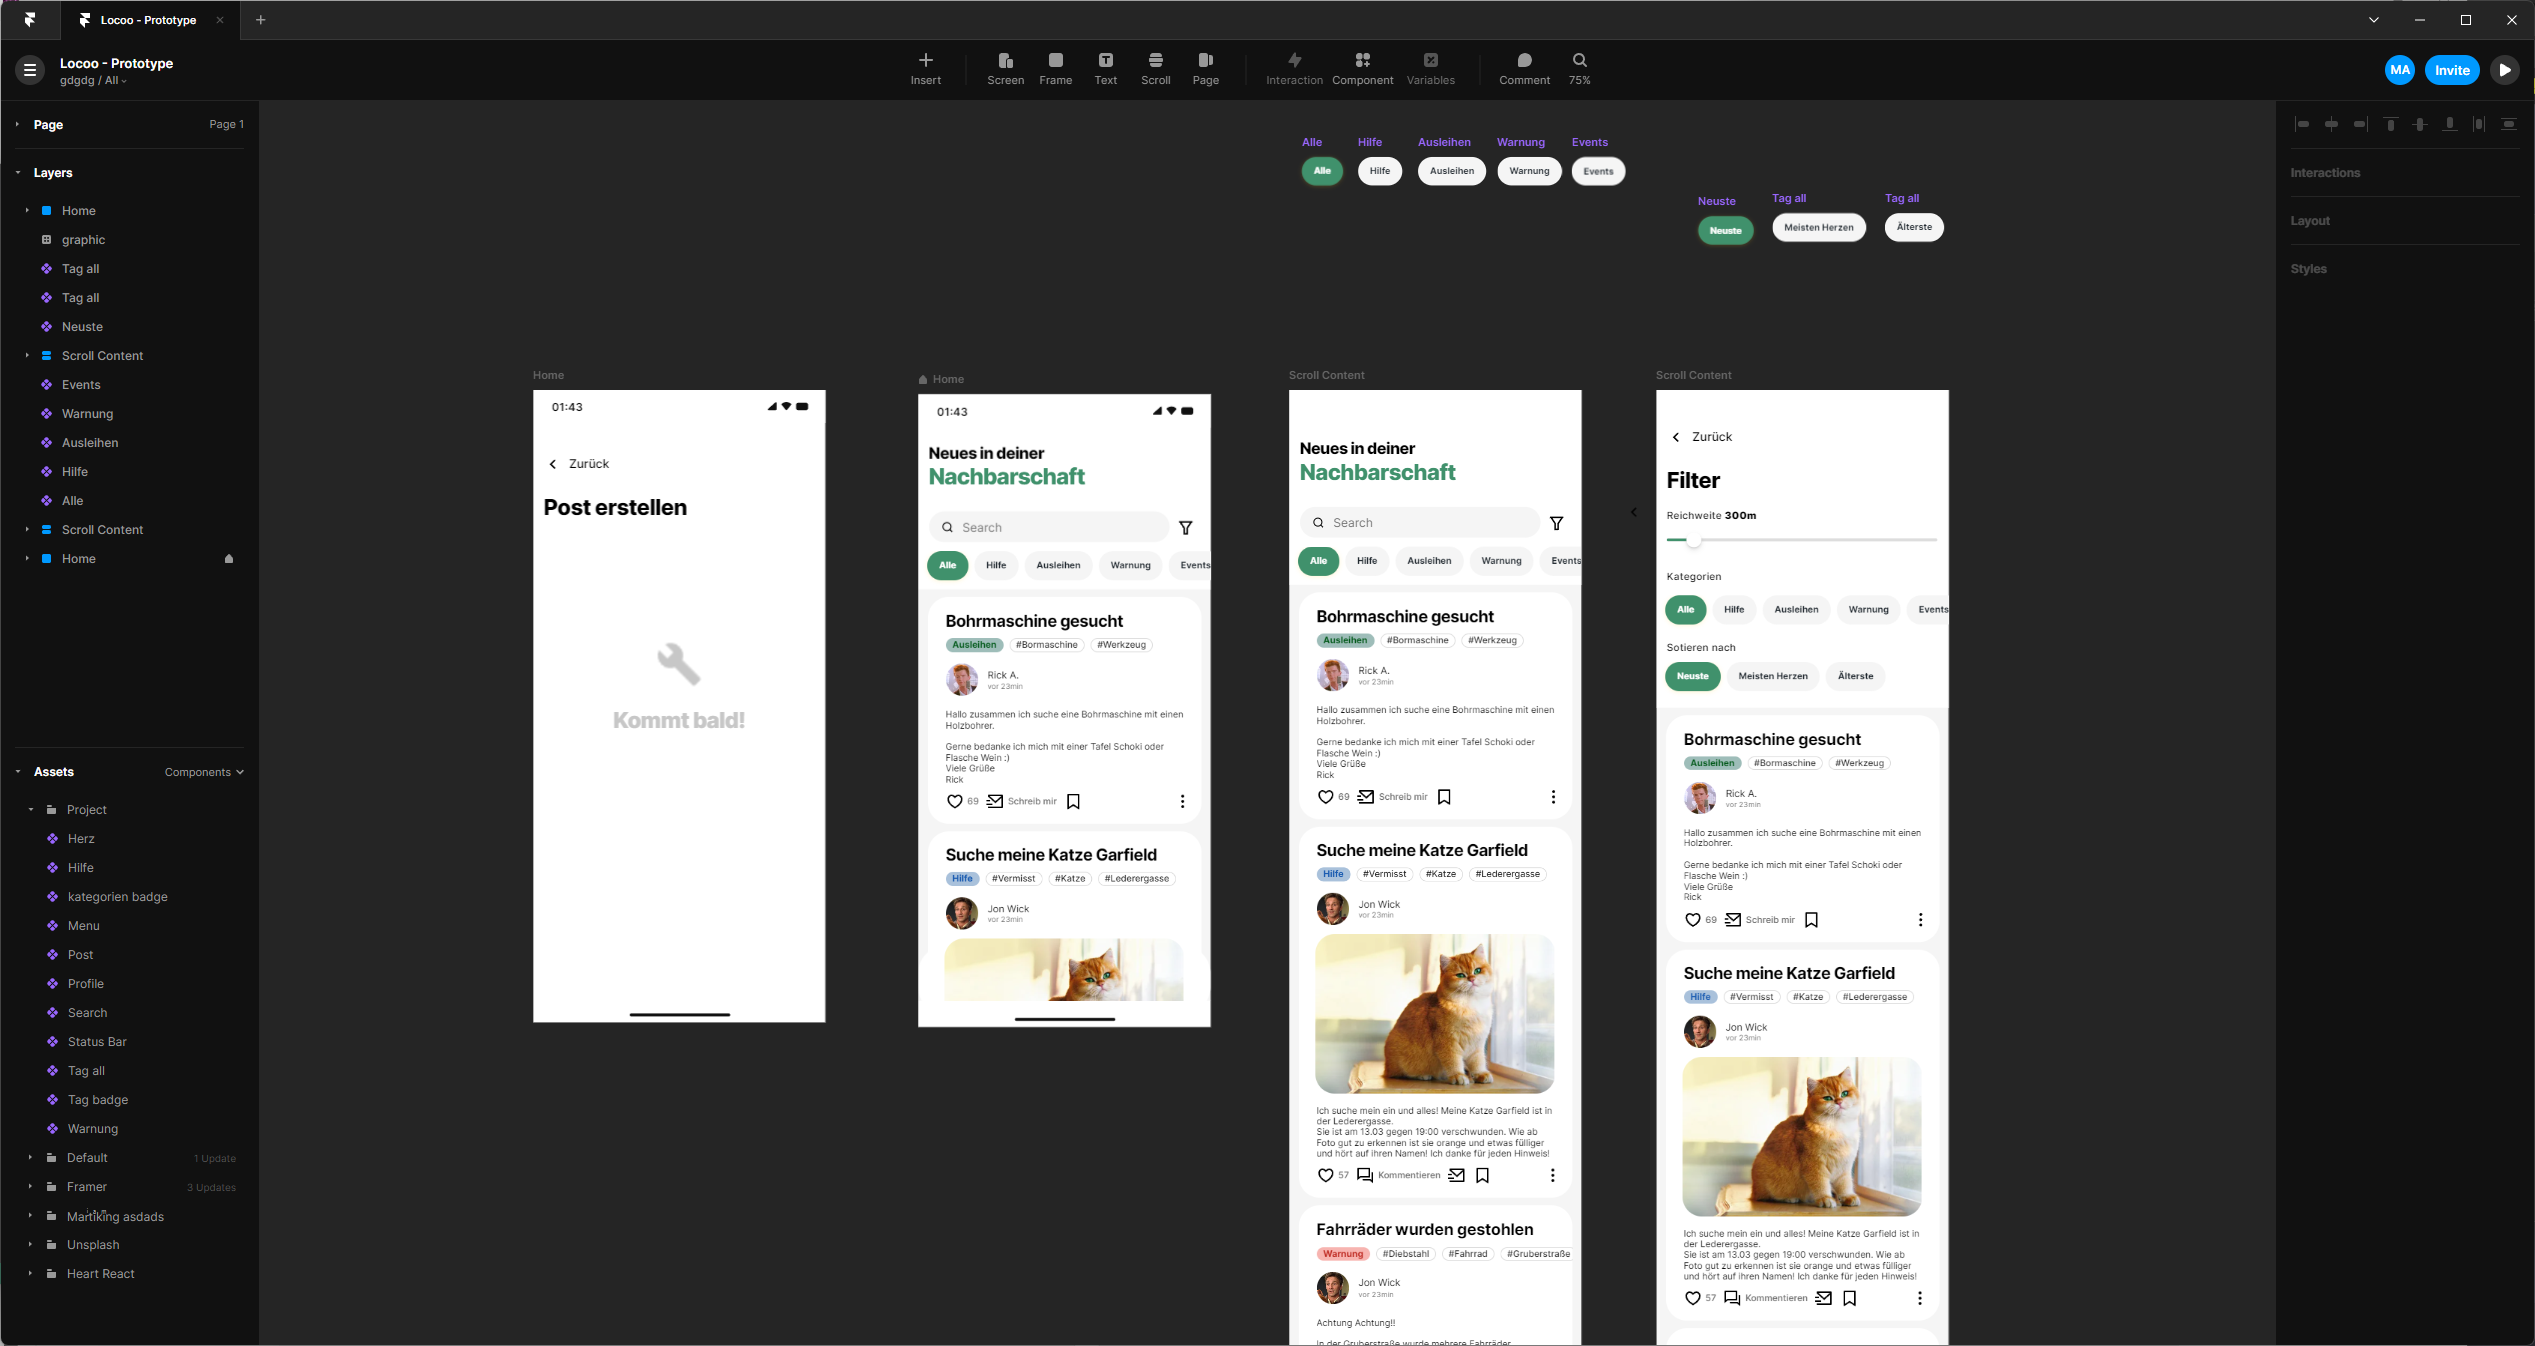
\includegraphics[width=1\textwidth]{pics/nochba-framer-prototype-screenshot.png}
  \caption{Nochba Prototyp in Framer}
  \label{fig:framer-prototype}
\end{figure}


Framer wurde während des Hackerthon Linz haCKt verwendet, um
den ersten Prototypen zu erstellen wie bei der man bei der
Abbildung \ref{fig:framer-prototype} erkennen kann. Die Wahl von Framer war
aufgrund seiner Geschwindigkeit und Effizienz in der
Erstellung von funktionsfähigen App-Designs und der
Erfahrung, die der Benutzer bereits mit dem Tool hatte,
getroffen worden.

Seit der Erstellung des ersten Prototyps hat sich das Geschäftsmodell von Framer jedoch geändert. Es ist jetzt ein Website-Baukasten, der es Benutzern ermöglicht, einfach und schnell ansprechende Websites zu erstellen, ohne Kenntnisse in der Webentwicklung zu benötigen. Obwohl es nun als Website-Baukasten fungiert, behält Framer immer noch einige seiner Kernfunktionen als Prototyping-Tool bei, was es zu einer guten Option für Designer und Entwickler macht, die schnell Prototypen erstellen möchten.

Insgesamt hat Framer gezeigt, dass es ein schnelles und effektives Tool ist, um Designideen in die Tat umzusetzen. Obwohl es nun als Website-Baukasten fungiert, ist es immer noch eine nützliche Option für Designer und Entwickler, die schnell und einfach Prototypen erstellen möchten.

\subsubsection{Adobe XD}
Bei der ersten Nutzung von Framer wurden zahlreiche Funktionen und Optionen entdeckt, was zunächst begeisterte. Doch mit der Zeit wurde erkannt, dass dies für das betreffende Projekt zu umfangreich war und somit nach einer einfacheren Lösung gesucht werden musste. Die Wahl fiel auf Adobe XD, da bereits jahrelange Erfahrung mit diesem Tool vorhanden war.

Trotz des geringeren Funktionsumfangs im Vergleich zu Framer
ist Adobe XD aufgrund seiner Benutzerfreundlichkeit und
Einfachheit ein ideales Werkzeug, um schnell Prototypen zu
erstellen. Alle Hauptscreens wurden fertiggestellt wie man
bei Abbildung \ref{fig:adobexd-prototyp} sehen kann, bevor
die Entwicklung mit Flutter begann. Die anderen wichtigen
Screens wurden später gestaltet, nachdem eine bessere
Kenntnis von Flutter erlangt wurde und es möglich war, den
Aufwand für die Umsetzung besser abzuschätzen.

\begin{figure}[h]
  \centering
  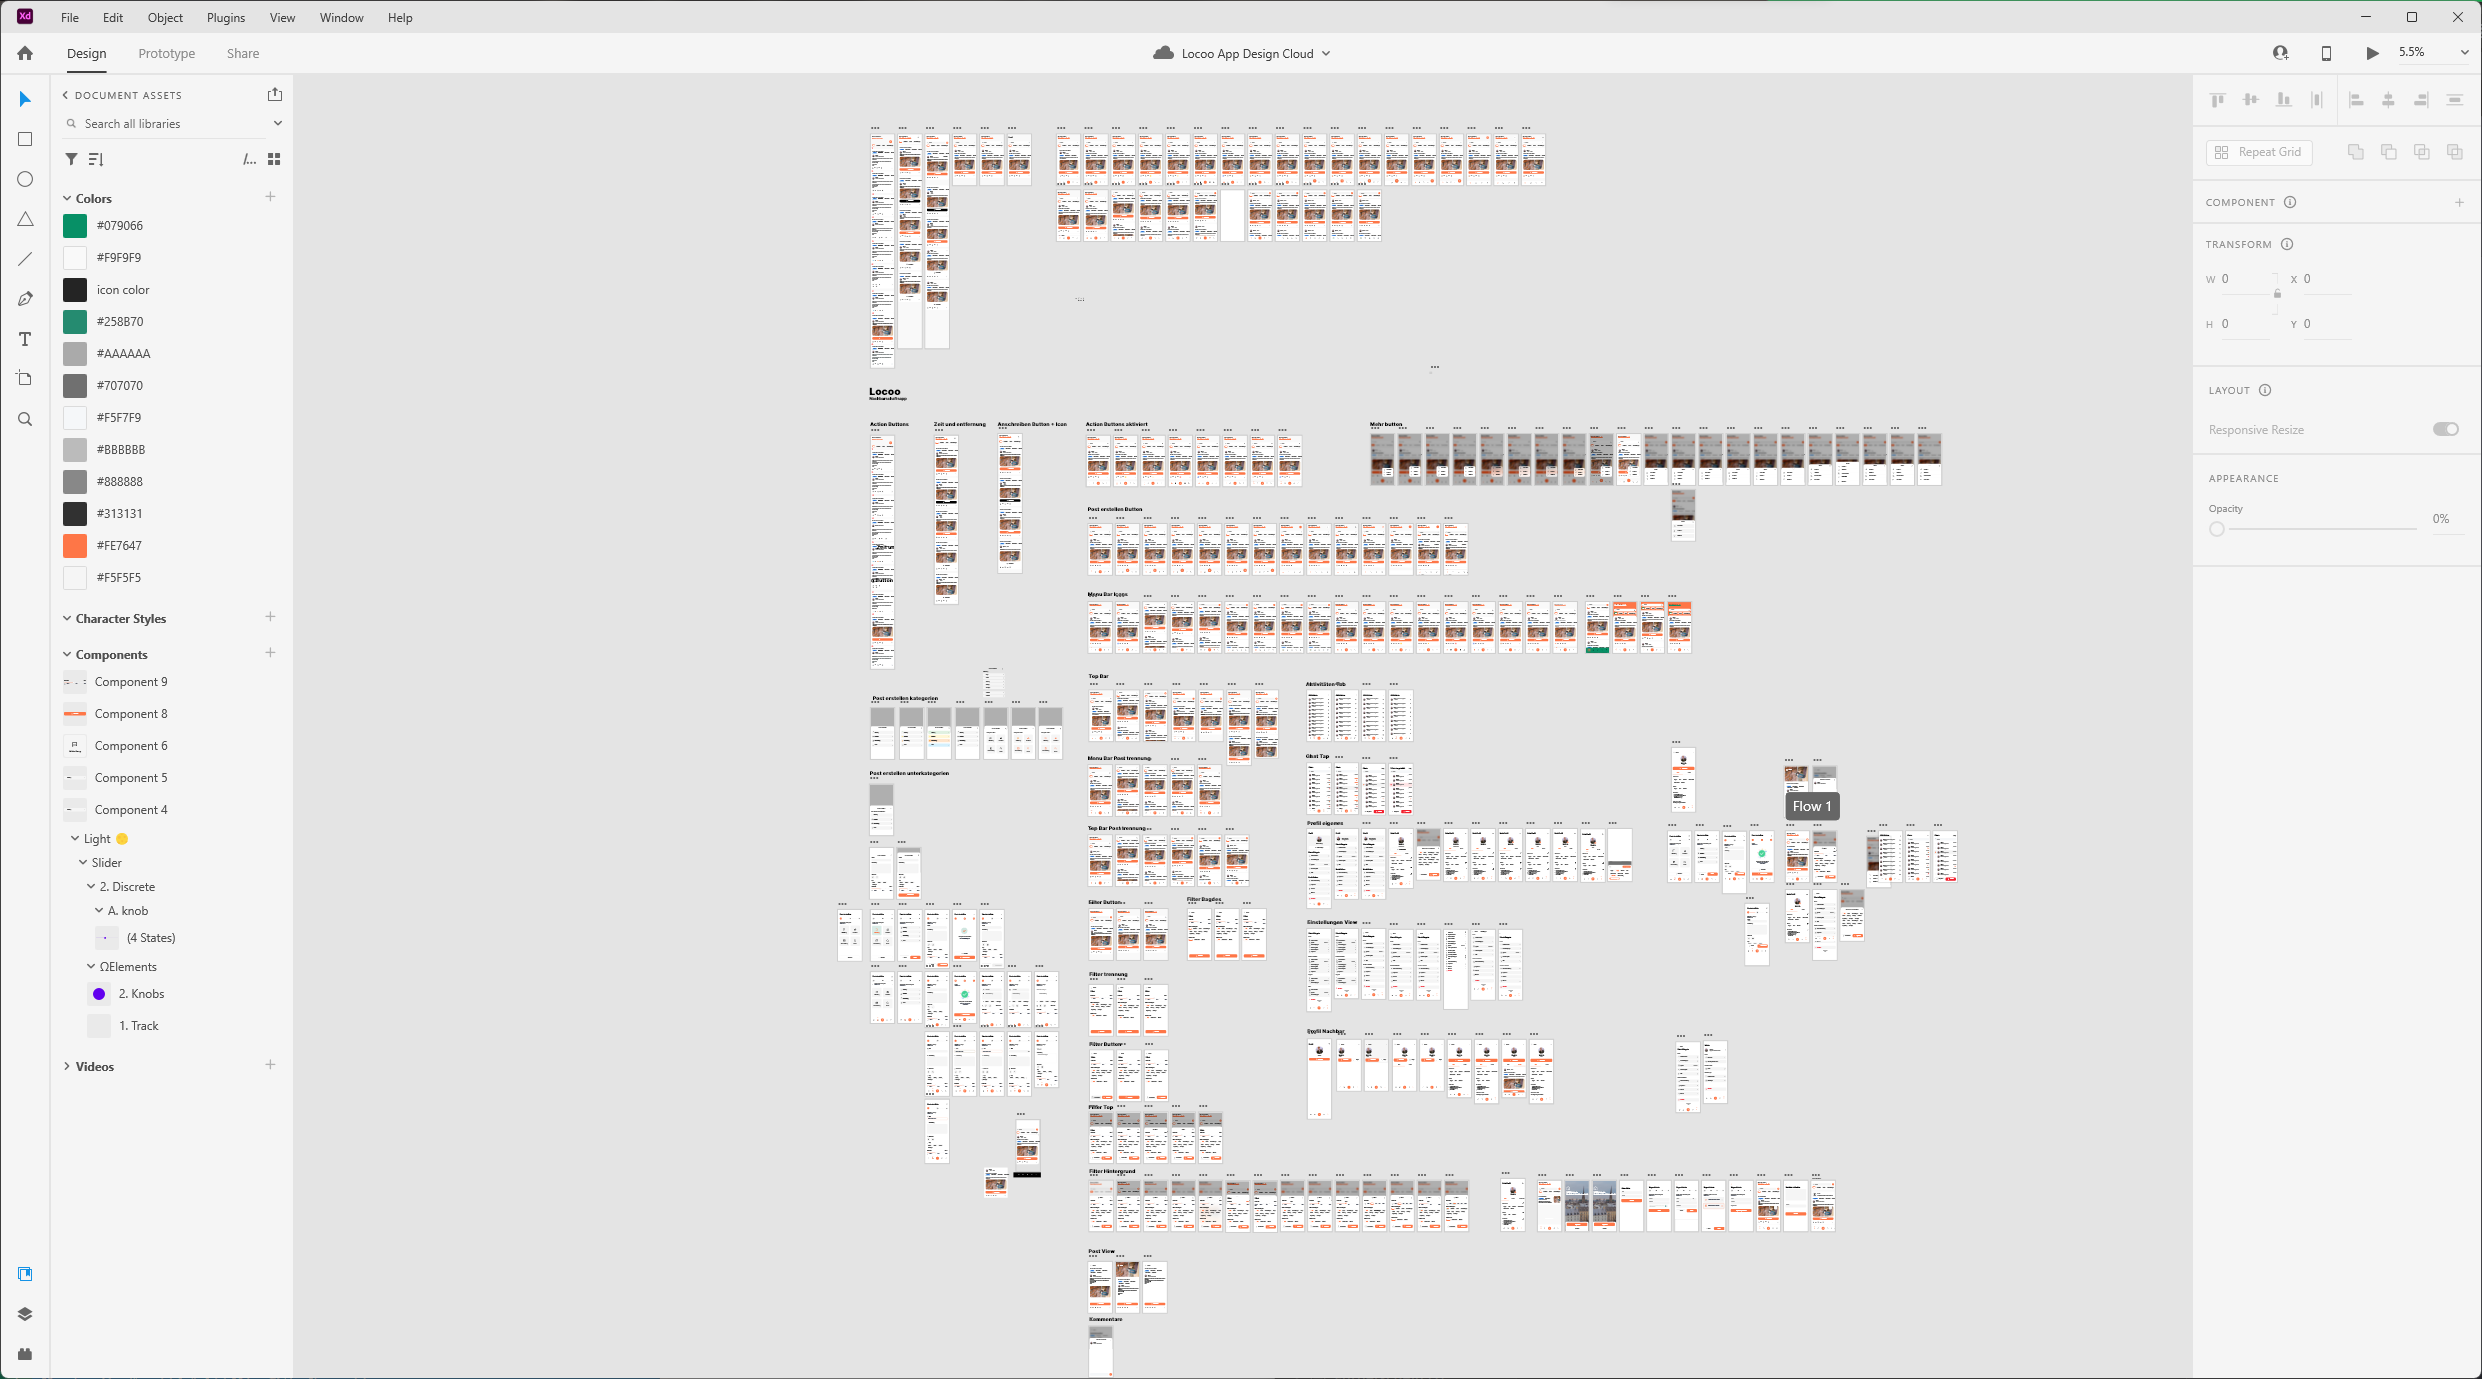
\includegraphics[width=0.95\textwidth]{pics/nochba-adobe-xd-protoype-screenshot.png}
  \caption{Nochba Prototyp in Adobe XD}
  \label{fig:adobexd-prototyp}
\end{figure}

Die Abbildung \ref{fig:adobexd-prototyp} zeigt eine Sammlung von Designs und Designentwicklungen im Prototypen. Adobe XD erwies sich als passend für das Projekt, da Martin Hausleitner, der alleinige Designer, keine Kollaborationsfunktionen benötigte. Das Tool ermöglichte es ihm, verschiedene Designvarianten effizient zu entwickeln und zu optimieren, um eine ansprechende Benutzeroberfläche für die Anwendung zu erstellen.

Jedoch ist der Designer mit
dem bekannteren und kostengünstigeren Figma vertraut, das
bei der Zusammenarbeit an einem Design und aufgrund der
zusätzlichen Funktionen besser geeignet ist.

Zusammenfassend kann festgestellt werden, dass Adobe XD ein leistungsstarkes Tool für UI/UX-Designer ist, das einfach zu bedienen ist und für kleine bis mittelgroße Projekte geeignet ist. Obwohl es nicht so viele Funktionen wie andere Tools bietet, eignet es sich gut für die schnelle Erstellung von Prototypen und eine einfache Zusammenarbeit mit Entwicklern und Stakeholdern.

\subsubsection{Design System}
\begin{figure}[h]
  \centering
  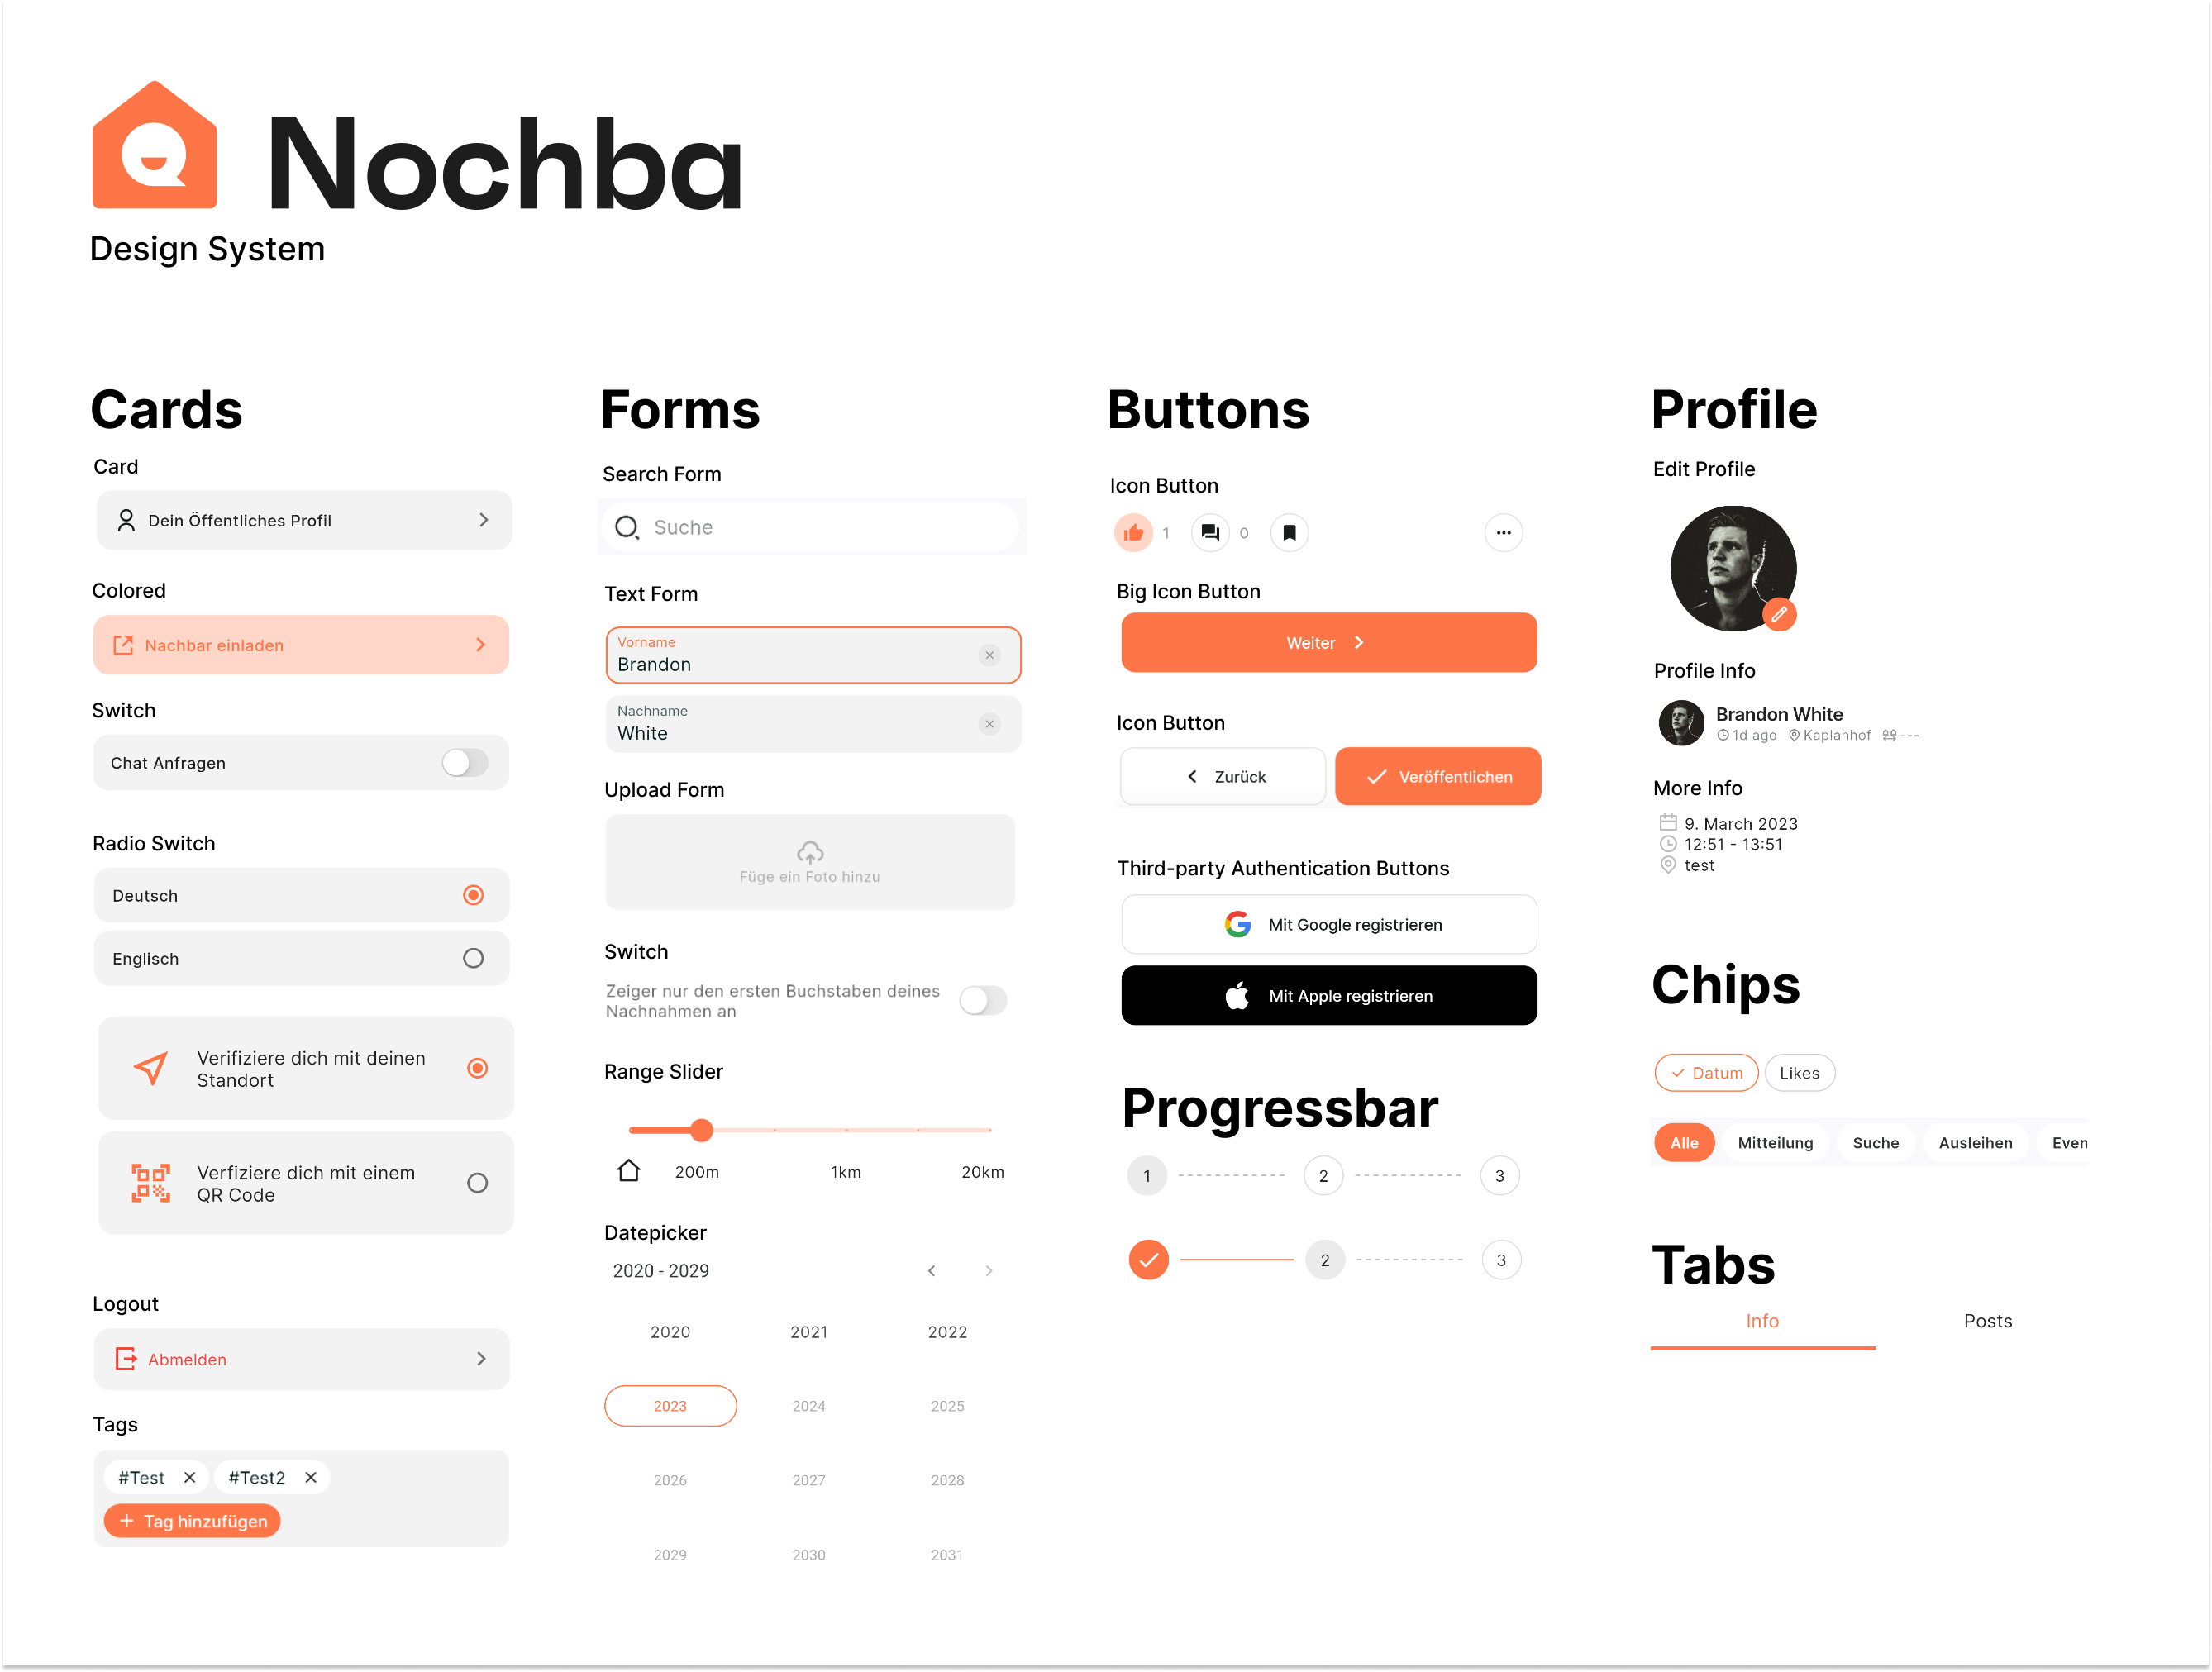
\includegraphics[width=1\textwidth]{pics/design-system.png}
  \caption{Nochba Design System}
  \label{fig:design-system}
\end{figure}

Der Designer Martin Hausleitner hat ein Design-System
entwickelt, um bei der Gestaltung der App eine klare
Struktur zu haben. Das System umfasst verschiedene
UI-Elemente, von denen die wichtigsten in Abbildung
\ref{fig:design-system} dargestellt sind.

\paragraph{Cards}

Ein häufig genutztes UI-Element in der App ist das Card-Design. Der Designer hat hierbei darauf geachtet, alle Elemente in einem abgerundeten, grauen Container mit hellem Grau zu gestalten, um einen guten Kontrast zum Hintergrund zu erzeugen.

Um den Nutzer zur Interaktion aufzufordern, wurde beispielsweise eine Einladungskarte für Nachbarn gestaltet, die in den Primär- und Sekundärfarben gehalten ist.

Für die Switch Card wurde das Switch-Design des verfügbaren Cupertino UI-Widgets genutzt, da es dem Designer gut gefiel.

Für den Radio Switch gibt es eine größere und eine kleinere Variante, um verschiedenen Design-Anforderungen gerecht zu werden.

Der Logout-Button wurde bewusst mit einem roten Icon und roter Schrift gestaltet, um dem Nutzer deutlich zu machen, dass er sich ausloggt.

Besondere Aufmerksamkeit erforderte der Tag-Editor, der einer der aufwändigsten Widgets in Flutter war. Der Designer hat diesen komplett neu durchdacht, um das Erstellen und Abspeichern von Tags leicht verständlich zu gestalten, so dass jeder Nutzer damit umgehen kann.

\paragraph{Forms}
Das Suchformular wurde mit einem organisch runden Design gestaltet, das zum Feed-Screen der App passt. Die Formulare, die in der gesamten App verwendet werden, wurden in Flutter sehr aufwändig gestaltet, um den Vorgaben des Designers zu entsprechen.

Um dem Nutzer eine klare Rückmeldung zu geben, wurde ein
orangefarbener Ring um das angeklickte Feld platziert. Es
wurde darauf geachtet, dass das Label des Textfeldes immer
gut lesbar ist auch wenn Cursor innerhalb des Feldes
ist. Zudem wurde ein X-Button hinzugefügt, der den gesamten
Inhalt des Textfelds löscht.

Darunter befindet sich ein Upload-Formular, das im Design einer großen Card gestaltet ist, um dem Nutzer das Klicken zu erleichtern.

Der Switch, der in den Formularen verwendet wird, wurde aus dem iOS-Design übernommen.

Der Range-Slider wurde unter Verwendung des Material Designs gestaltet und mit den passenden Farben angepasst. Zusätzlich wurden Labels hinzugefügt, um dem Nutzer eine bessere Orientierung zu ermöglichen.

Für den Datepicker wurde die Bibliothek
\href{https://pub.dev/packages/syncfusion_flutter_datepicker}{Syncfusion\_flutter\_datepicker}
verwendet. Das UI wurde entsprechend den Farben der App
angepasst, um eine konsistente und ästhetische
Benutzeroberfläche zu gewährleisten.

\paragraph{Buttons}
Die Icon-Buttons stellten das aufwändigste Design-Element
dar, da es bei Flutter mehrere Möglichkeiten gibt, um sie zu
implementieren. Dies führte dazu, dass sie häufig geändert
werden mussten, um das richtige Design zu finden. Die
runden Icon-Buttons ziehen sich durch die gesamte App.

Der Big Icon Button wurde häufig eingesetzt, da er die Primary Color aufweist und somit eine wichtige Funktion anzeigt. Dem Designer war es wichtig, dass jeder Button immer ein Icon hatte, um dem Nutzer die Bedienung zu erleichtern. Es wurde darauf geachtet, dass alle Buttons die gleiche Rundung aufweisen.

Für den normalen Icon-Button wurde ein dezenter grauer Hintergrund verwendet, um ihn als Secondary Button zu kennzeichnen. Auch hier wurden immer Icons verwendet.

In der App wurden zusätzlich Third-Party-Anmeldemöglichkeiten Buttons integriert. Dazu gehören das Login mit Apple und das Login mit Google. Um eine konsistente Benutzeroberfläche sicherzustellen, wurden diese Anmeldeoptionen entsprechend an das Design angepasst.

Die Progressbar wurde beim Registrierungsprozess und beim
Erstellen eines Posts eingesetzt, um dem Nutzer eine bessere
Orientierung zu geben, wie viele Schritte noch zu erledigen
sind. Ursprünglich war geplant, das Design von Material zu
nutzen. Aufgrund der Einschränkungen bei der Umsetzung des
Designs mit dem Material-Design in Flutter und den spezifischen
Anforderungen des Designers, war es erforderlich, die
Progressbar komplett in Flutter zu gestalten.

\paragraph{Profile}

Der Edit Profile-Button wurde beim Registrieren und
Bearbeiten eines Profils verwendet, um das Profilbild
zu ändern. Es wurde darauf geachtet, dass der Button
auffällig ist, damit der Nutzer ihn schnell erkennen kann.

Die Profil-Informationen werden bei jedem Beitrag angezeigt,
darunter die Zeit, in welchem Stadtteil der Nachbar wohnt
und die ungefähre Entfernung zu ihm. Es wurde darauf
geachtet, dass die Informationen übersichtlich mit
Icons dargestellt werden, um dem Nutzer eine schnelle Orientierung
zu ermöglichen.

More Info wird beispielsweise bei einem Event-Eintrag oder
den persönlichen Daten eines Profils verwendet. Hier wurden
Icons verwendet, um dem Nutzer eine einfache und
verständliche Darstellung zu ermöglichen.

\paragraph{Chips}
Chips kommen in der App häufig zum Einsatz, um Filter auszuwählen. Der Designer ist allerdings mit dem finalen Design noch nicht vollständig zufrieden, da es zahlreiche unterschiedliche Varianten gibt. Die Gestaltung der Chips wird weiterhin optimiert, um eine einheitliche und ästhetisch ansprechende Darstellung zu erreichen. Dieser fortlaufende Prozess zeigt das Bestreben, die Benutzeroberfläche kontinuierlich zu verbessern und den Anforderungen der Benutzer gerecht zu werden.

\paragraph{Tabs}
Die Implementierung von Tabs war auch in Flutter eine
Herausforderung, da die Positionierung nicht der
Standard-Tabs-Position entsprach. Aus diesem Grund wurde die
Gestaltung aufwändig gestaltet, um ein optimales Ergebnis zu
erzielen. Die Mühe hat sich jedoch gelohnt, da die Tabs nun
eine gute funktionale Benutzeroberfläche bieten.

\subsubsection{Farben}
Die Farbpalette einer Marke spielt eine wichtige Rolle im UI-Design, da sie dazu beiträgt, ein konsistentes Erscheinungsbild zu schaffen. Bei der Gestaltung einer Nachbarschafts-App wurde eine Vielzahl von Farbpaletten von anderen Apps untersucht. Es wurde festgestellt, dass die meisten großen Apps die Farbe Grün verwenden.

Obwohl Grün oft mit Natur und Gemeinschaft assoziiert wird, wurde sich bewusst dazu entschieden, sich von diesen etablierten Konventionen abzuheben. Stattdessen wurde die Farbe Orange ausgewählt, da sie auffällig und ungewöhnlich ist und somit das Potenzial hat, die App von anderen Nachbarschafts-Apps zu unterscheiden.

Zusätzlich passt die Farbe Orange gut zu den Werten der App, da sie für Wärme, Freundschaft und Optimismus steht - Eigenschaften, die in der App gefördert werden sollen. Die Hoffnung besteht darin, dass die Farbauswahl dazu beitragen wird, dass die Nutzer sich in der App wohl und willkommen fühlen und die Farbe sich als wiedererkennbares Markenzeichen etabliert.


\begin{figure}[h]
  \centering
  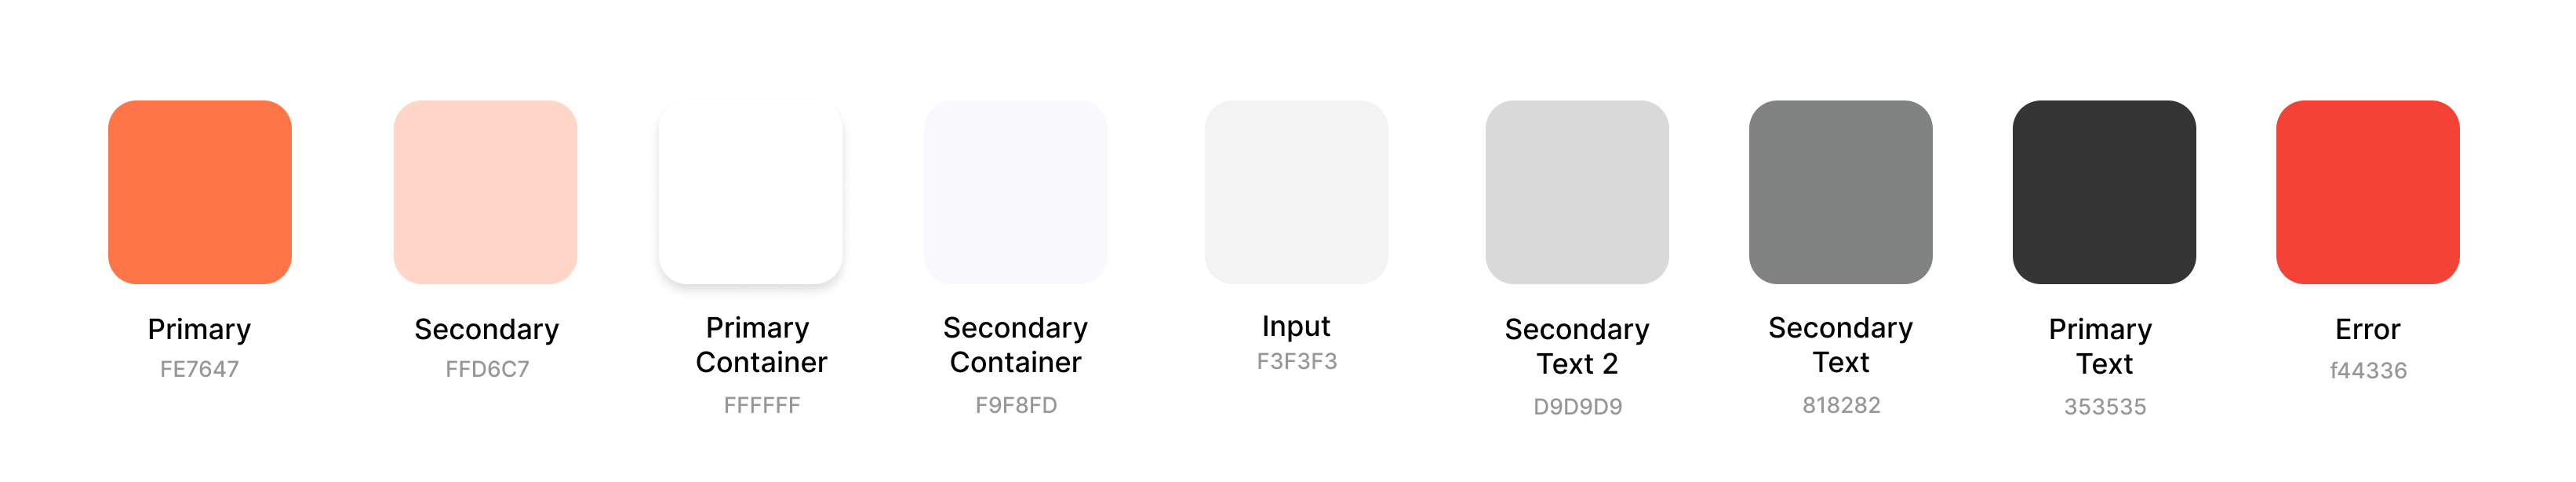
\includegraphics[width=1\textwidth]{pics/colors.png}
  \caption{Nochba Farbpalette}
  \label{fig:color-chart}
\end{figure}

Bevor der endgültige Farbton ausgewählt wurde, wurden verschiedene orangefarbene Töne für den Prototypen ausprobiert und für einige Tage beobachtet, um ein Gefühl für die Farbe zu bekommen. Schließlich wurde sich für die endgültigen Farben entschieden, wie in der Abbildung \ref{fig:color-chart} dargestellt.

Die Hauptcontainerfarbe für die meisten Ansichten ist Weiß, ebenso wie die Hintergrundfarbe der Posts. Allerdings wurde eine Farbe gesucht, die gut als Hintergrund passt, weshalb ein helles Grau verwendet wurde.

Für die Textfarbpalette wurde fast Schwarz gewählt, da dies zu einem weicheren Eindruck führt. Um Untertitel weniger präsent zu gestalten, wurde ein etwas hellerer Grauton gewählt.


\subsubsection{Icons}


\begin{figure}[ht]
  \centering
  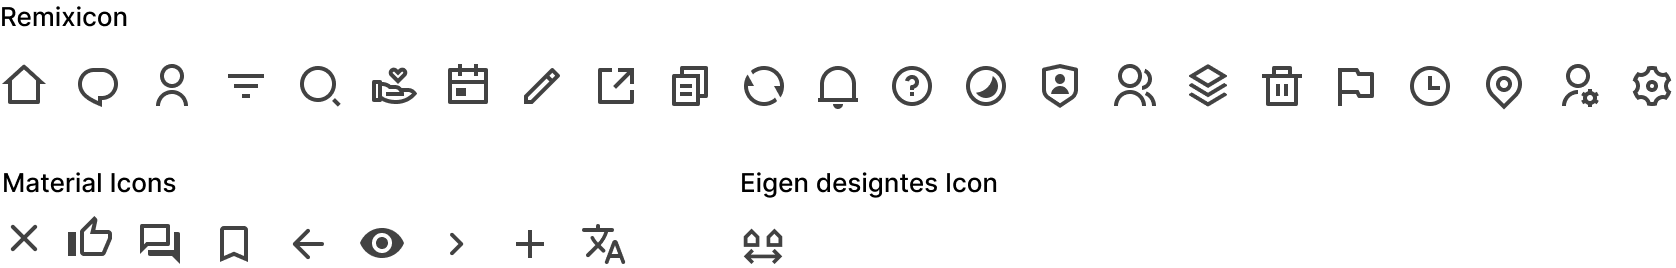
\includegraphics[width=1\textwidth]{pics/icons.png}
  \caption{App Icons}
  \label{fig:app-icons}
\end{figure}

Die obige Abbildung \ref{fig:app-icons} zeigt alle Icons,
die in einer App verwendet werden. Das Ziel war es, eine
möglichst große Anzahl von Icons zu integrieren, um die
Benutzerfreundlichkeit und Bedienbarkeit der App zu
verbessern. Nachdem verschiedene Icon-Packs betrachtet
wurden, wurde hauptsächlich das frei verfügbare
\href{https://github.com/Remix-Design/remixicon}{Remixicon}-Pack
verwendet, um der App ein einzigartiges Aussehen zu
verleihen und sie von anderen Apps abzuheben. Das runde
Design der Icons wurde besonders geschätzt. Ein weiterer
Vorteil von Remixicons ist, dass es ein
\href{https://pub.dev/packages/remixicon}{Flutter-Package}
gibt, was
die Implementierung erleichtert hat.

Obwohl Remixicons viele Icons zur Verfügung stellt, wurden
bei einigen Icons die
\href{https://fonts.google.com/icons?icon.set=Material+Icons}{Material Icons}
von Google bevorzugt.
Insbesondere die abgerundeten Icons wurden verwendet, um das
Design insgesamt weicher zu gestalten. Da kein passendes
Icon vorhanden war, um den Abstand zwischen zwei Nachbarn zu
symbolisieren, wurde ein neues Icon im Stil der anderen
entworfen.

\subsubsection{Typografie}
\begin{figure}[H]
  \centering
  
\includegraphics[width=1\textwidth]{pics/font.png}
  \caption{Die Schriftfamilie Inter}
  \label{fig:font}
\end{figure}

Ein wichtiger Teil jedes Designs ist die Typografie, so auch bei der Nochba-App.

Der Designer der App war auf der Suche nach einer
Schriftart, die modern, ansprechend und gut lesbar ist. Er
suchte nach einer Schriftart, die Lesbarkeit und das
Verständnis des Textes verbessert. Schließlich stieß er auf
die Schriftart "Inter" von Rasmus Andersson
\cite{inter-font}, die man auf der Abbildung \ref{fig:font}
betrachten kann.

Inter ist eine moderne und ansprechende Schriftart, die speziell für die Verwendung auf Bildschirmen entwickelt wurde. Die Schriftart ist in vielen verschiedenen Stilen verfügbar und bietet eine breite Unterstützung für verschiedene Sprachen und Schriftsysteme. Dies war besonders wichtig für den Designer der Nachbarschafts-App, da die App von Menschen aus verschiedenen Ländern genutzt wird, die möglicherweise unterschiedliche Sprachen und Schriftsysteme verwenden.

Ein weiterer Vorteil von Inter ist seine Lesbarkeit. Die Schriftart ist gut lesbar, auch in kleineren Größen, was besonders wichtig ist, da die App oft auf mobilen Geräten verwendet wird. Die klare und prägnante Schriftart von Inter verbessert auch die Lesbarkeit und das Verständnis des Textes, was wiederum zu einer besseren Benutzererfahrung führt.

Schließlich ist Inter auch eine Open-Source-Schriftart, die kostenlos verwendet werden kann \cite{inter-font}. Dies ist besonders wichtig für das Projekt Nochba, da Nochba für Open Source Stehen will.

Zusammenfassend lässt sich sagen, dass Inter eine ausgezeichnete Wahl für die Nachbarschafts-App ist. Die Schriftart ist modern, ansprechend und gut lesbar, und bietet eine breite Unterstützung für verschiedene Sprachen und Schriftsysteme. Die Verwendung von Inter hat dem Designer der App geholfen, eine professionelle und kosteneffektive Lösung für die Entwicklung der App zu finden.
\subsubsection{Logo}

\begin{figure}[h]
  \centering
  
\includegraphics[width=0.95\textwidth]{pics/final-logo.png}
  \caption{Finales Logo}
  \label{fig:final-logo}
\end{figure}

% 
\includegraphics[width=0.35\textwidth]{pics/app-logo.png}

% überschrift logo historie
\paragraph{Logo Historie}

\begin{figure}[h]
  \centering
  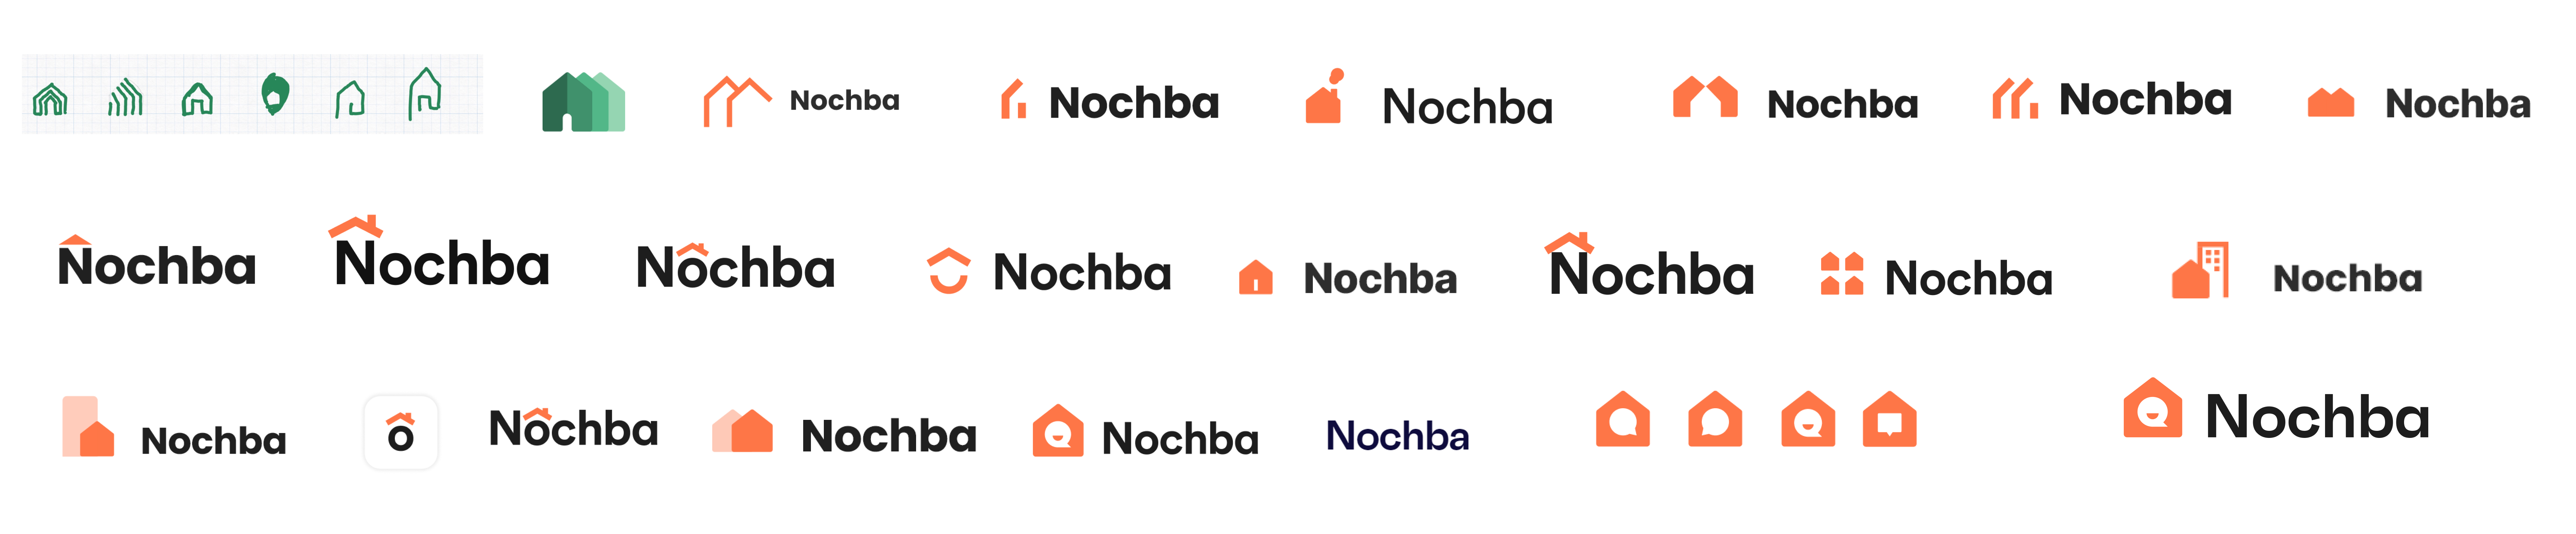
\includegraphics[width=0.95\textwidth]{pics/logo-historie.png}
  \caption{Logo Design Ideen}
  \label{fig:logo-historie}
\end{figure}

Im Zuge des Designprozesses wurden hohe Ansprüche an das
Logo der App gestellt, da es das Projekt repräsentiert und
es dem Team wichtig ist. Es
war wichtig, dass das Logo einfach gehalten und leicht
erkennbar ist. Die endgültige Gestaltung des Logos hat viel Zeit
in Anspruch genommen, da die vorherigen Entwürfe nicht
vollständig zufriedenstellten die man bei Abbildung
\ref{fig:logo-historie} sieht. Nach anderen Logos, die eine
Verbindung zu Nachbarschaften oder Häusern herstellen, wurde
gezielt gesucht und Ideen auf dem Discord-Server
gespeichert. Es sollte immer ein Haus erkennbar sein, da
Häuser schnell mit Nachbarschaften in Verbindung gebracht
werden.

In den früheren Versionen der App gab es Schwierigkeiten,
ein ansprechendes App-Icon zu gestalten, da kein
eigenständiges Icon vorhanden war. Aus diesem Grund wurde
entschieden, den Schriftzug und das App-Icon (Logo) separat
zu gestalten, wie es auch bei anderen Apps üblich ist. Das
endgültige Logo wurde erst Ende 2022 entworfen, da alle
anderen Designs nicht gefielen. Es wurde ein Haus mit einer
sprechenden Sprechblase, die lächelt, als Logo
wie bei Abbildung \ref{fig:final-logo} zu sehen ist gewählt. Dies soll symbolisieren, dass
man innerhalb des Hauses sprechen kann und das Lächeln soll
verdeutlichen, dass man Freude mit seinen Nachbarn teilen
kann. Eine runde, verspieltere Schriftart wurde bewusst
gewählt, da sie besser mit der Farbmischung harmoniert als
die vorherige Schriftart.



\subsection{App Design}
\subsubsection{Thumb Zone Prinzip}
\begin{figure}[h]
  \centering
  \begin{minipage}[b]{0.3\textwidth}
    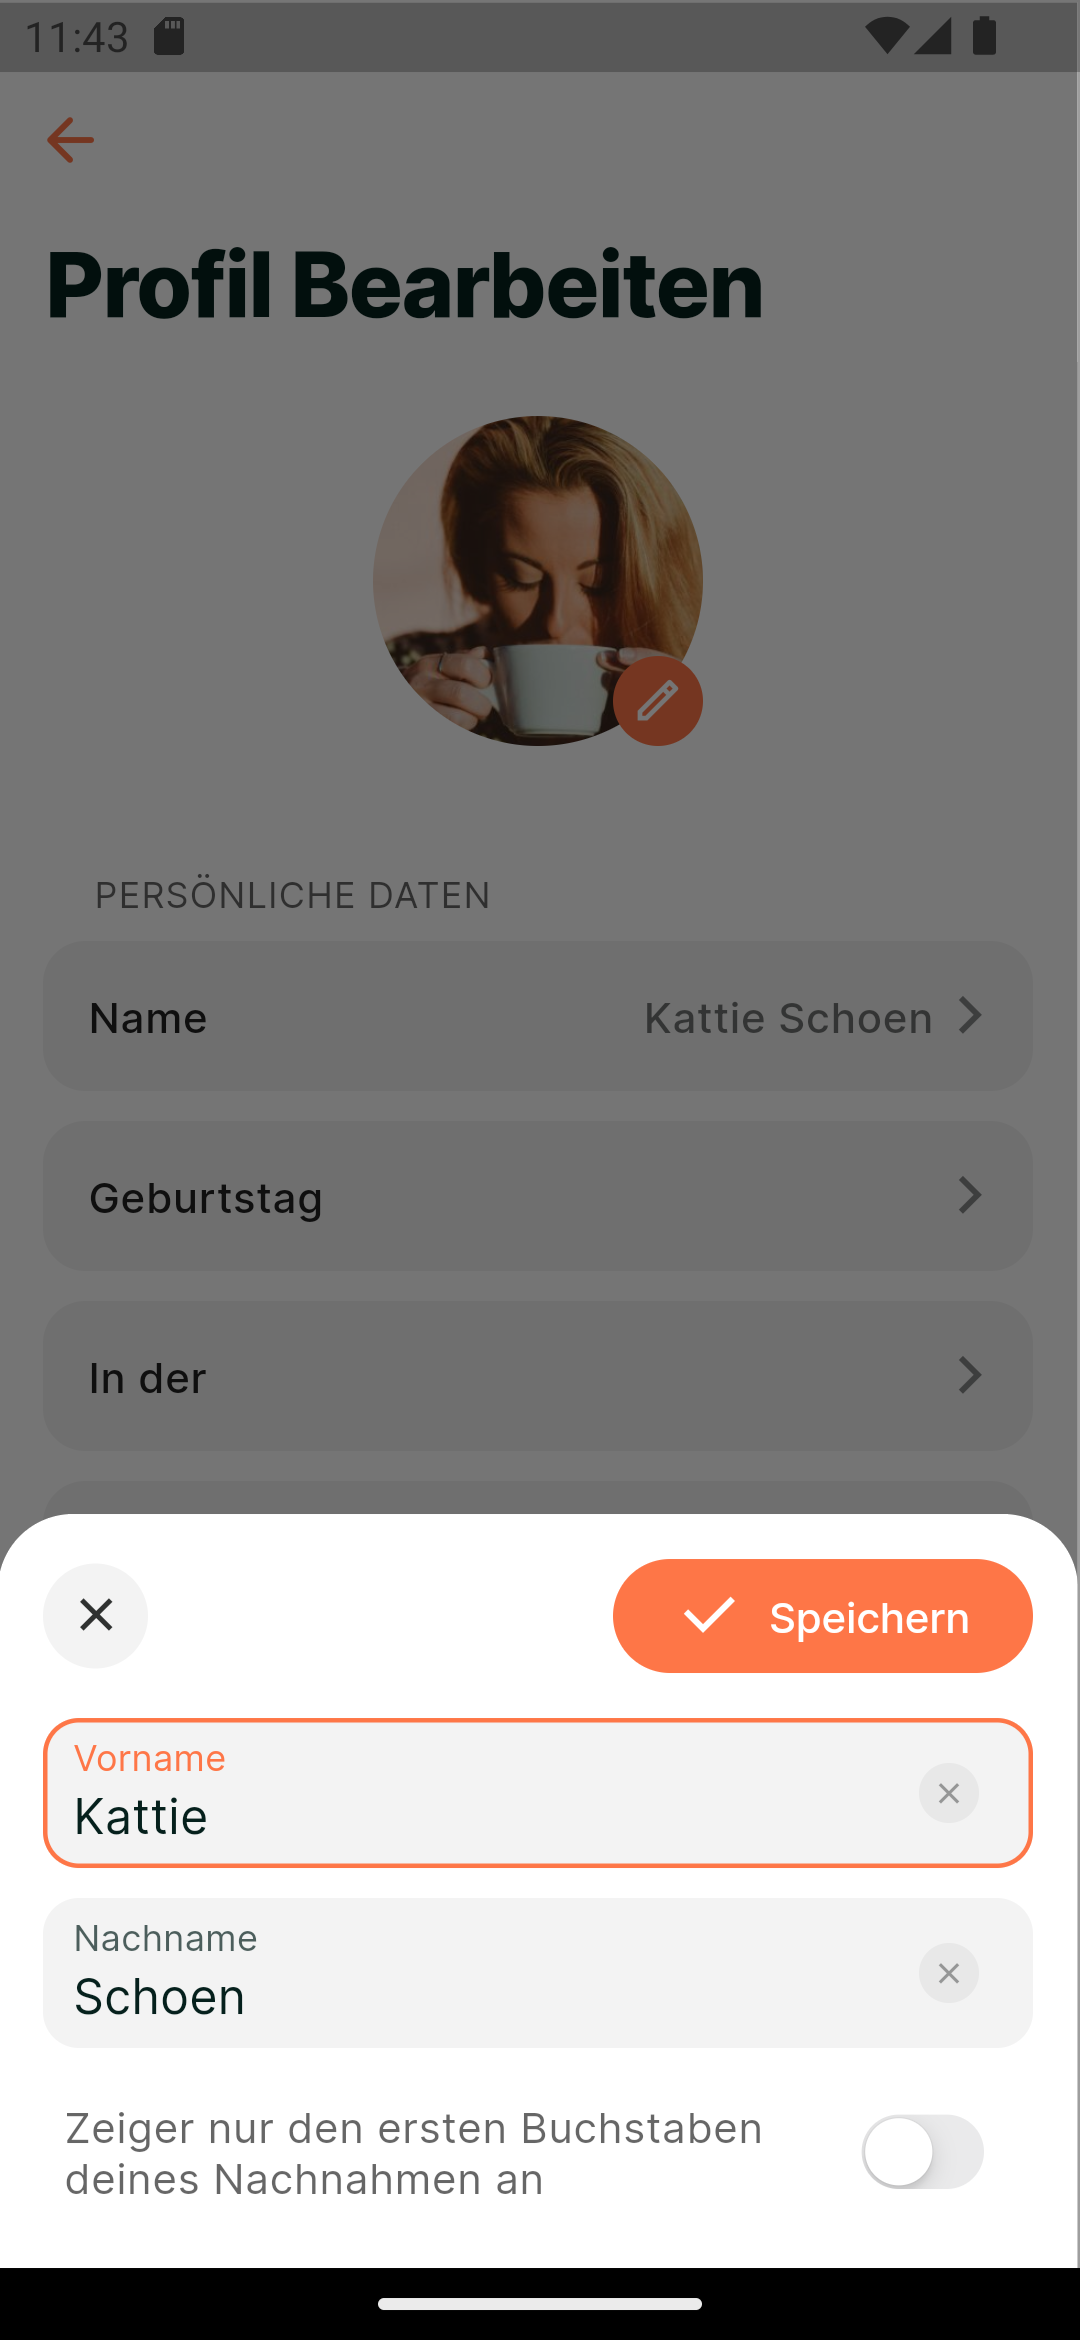
\includegraphics[width=\textwidth]{pics/edit-name-screen.png}
    \caption{Screenshot des "Name bearbeiten"-Screens}
    \label{fig:edit-name-screen}
  \end{minipage}
  \hfill
  \begin{minipage}[b]{0.3\textwidth}
    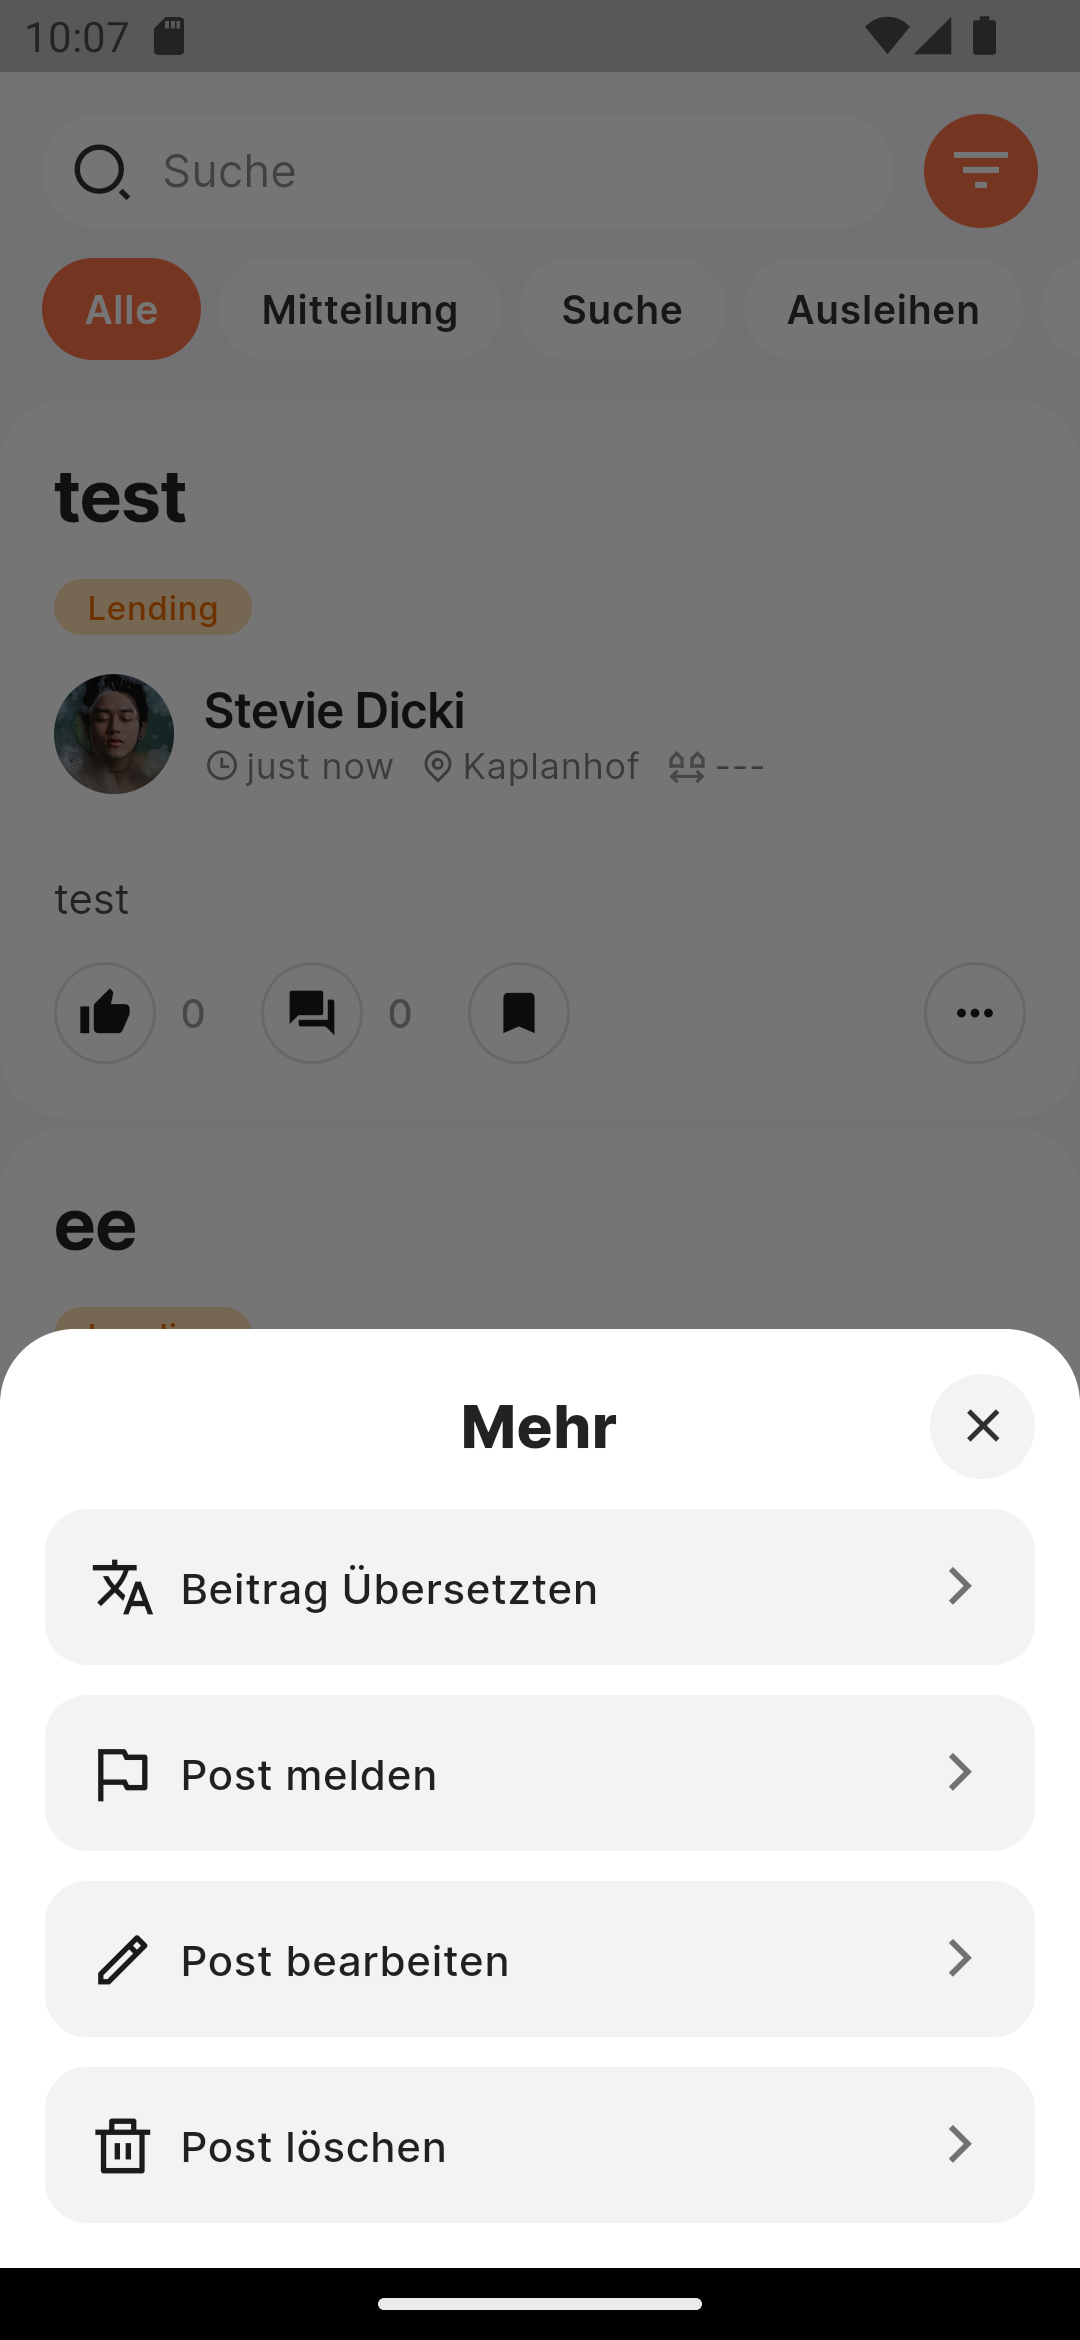
\includegraphics[width=\textwidth]{pics/post-more-menu.png}
    \caption{Screenshot des "Mehr"-Menüs für Beiträge}
    \label{fig:post-more-menu}
  \end{minipage}
  \hfill
  \begin{minipage}[b]{0.3\textwidth}
    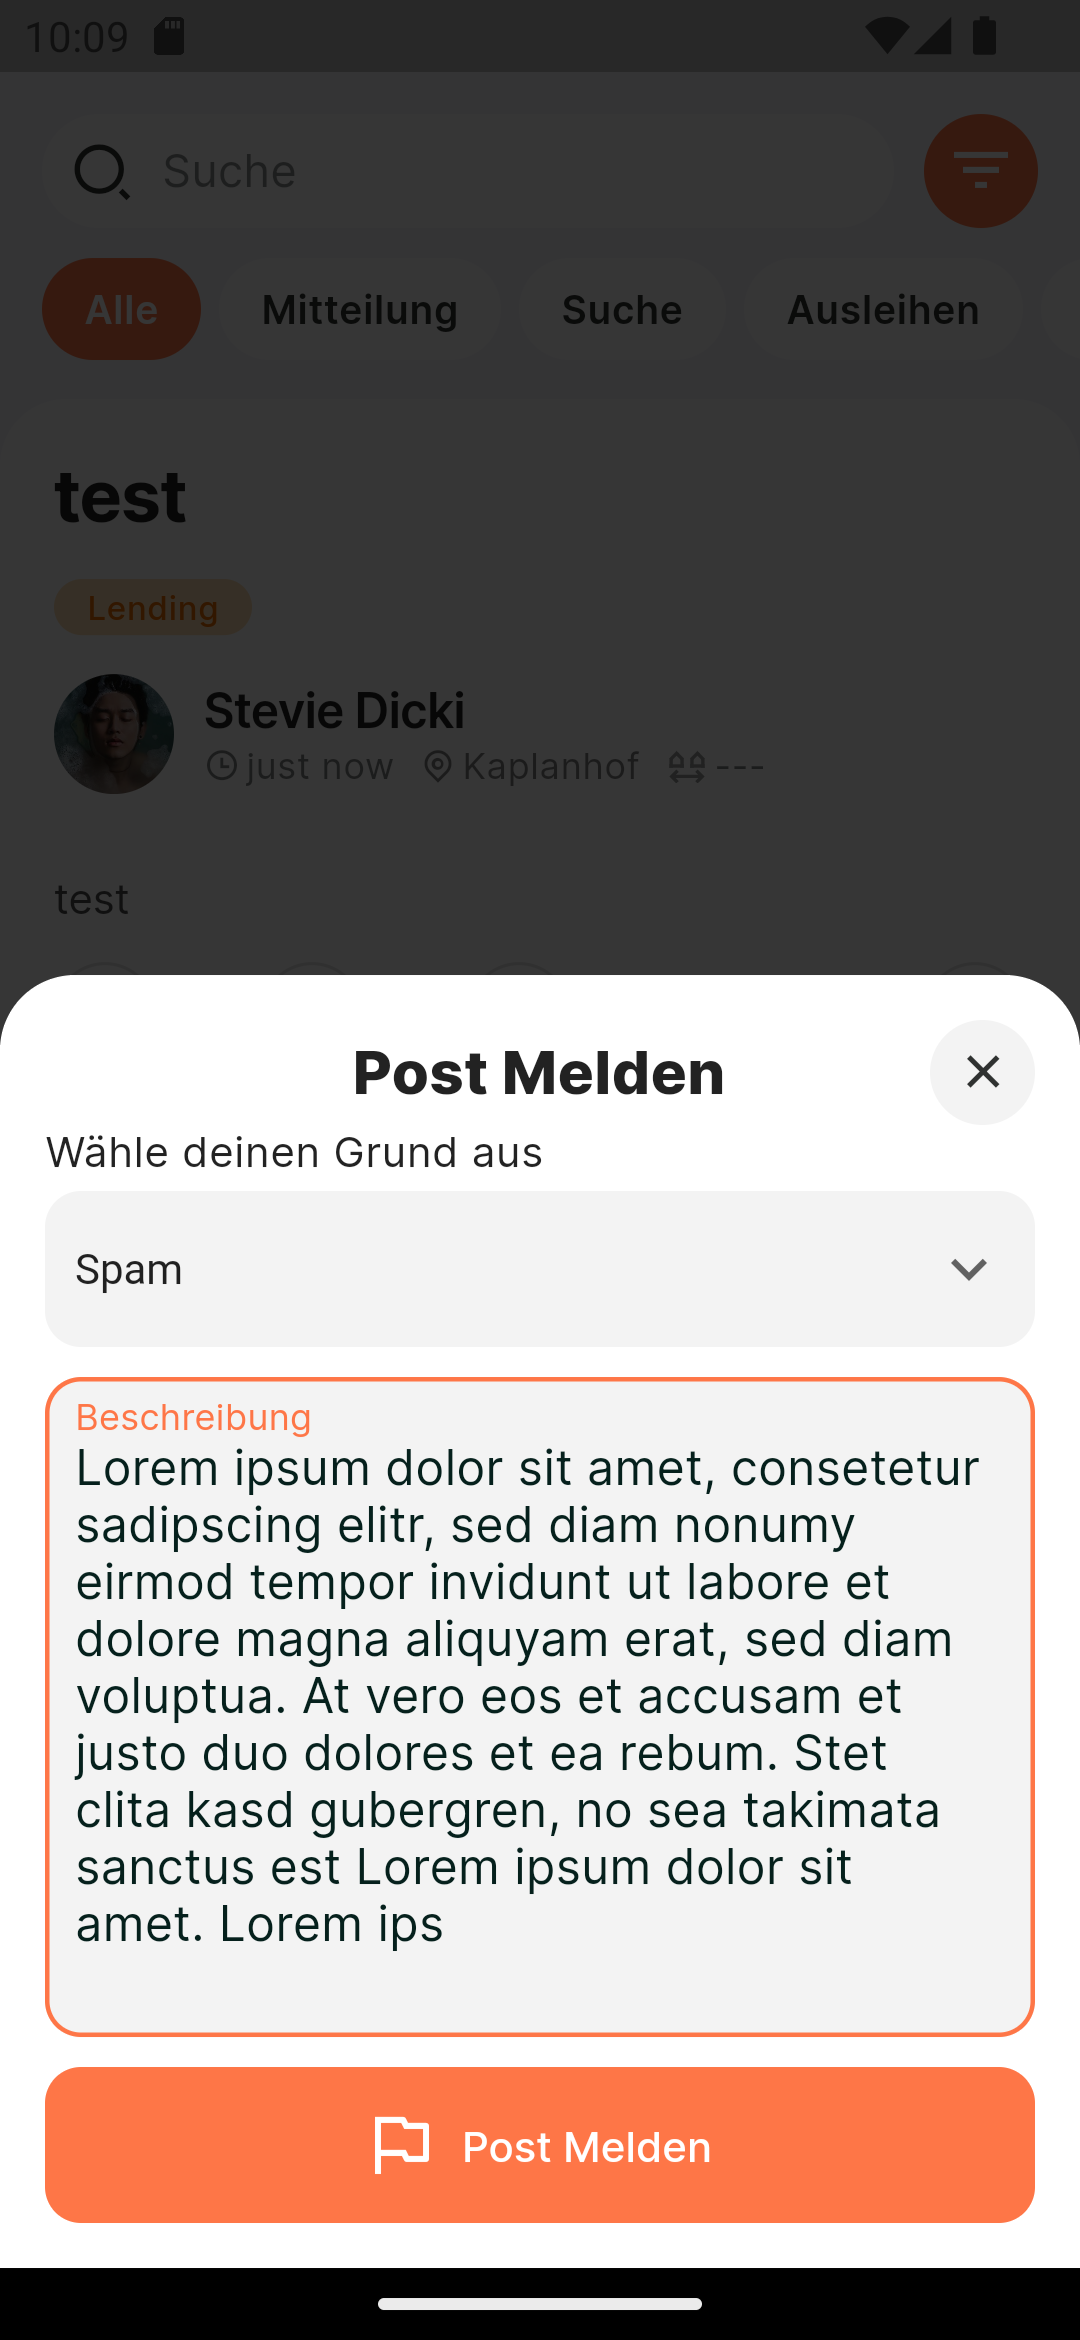
\includegraphics[width=\textwidth]{pics/post-report-menu.png}
    \caption{Screenshot des "Beitrag melden"-Menüs}
    \label{fig:post-report-menu}
  \end{minipage}
\end{figure}
Im Design-Muster wurde versucht, das Thumb Zone Prinzip zu
implementieren, indem wichtige UI-Elemente immer im unteren
Bereich der App platziert wurden. Das Layout für die
Namensbearbeitung \ref{fig:edit-name-screen} wurde extra
unten platziert, um alle Klick-Elemente bequem mit dem
Daumen bedienen zu können. Wichtige
wie "Speichern"
wurden in der primären Farbe gestaltet und rechts
ausgerichtet, um einen leichteren Zugriff zu gewährleisten.
Das Textfeld kann einfach durch Drücken der Enter-Taste auf
der Tastatur geändert werden, um das Eintippen von Daten zu
erleichtern.

Wie bei Abbildung \ref{fig:post-more-menu} \ref{fig:post-report-menu} zu sehen ist, erfolgt eine weitere Implementierung einer Bottom View, um dem Thumb Zone Prinzip gerecht zu werden.

Unwichtige Buttons wurden in grau gestaltet, wie z.B. der X-Button in der Abbildung. Ein Löschen-Button neben dem Textfeld wurde eingebaut, der es dem Benutzer ermöglicht, den gesamten Text bequem zu löschen. Jedoch war es nicht möglich, diese Prinzipien vollständig umzusetzen, da die Zeit gegen Ende knapp wurde. In zukünftigen Versionen der App soll sichergestellt werden, dass diese Prinzipien einheitlich angewendet werden.
\subsubsection{Design Historie}

\begin{figure}[h]
  \centering
  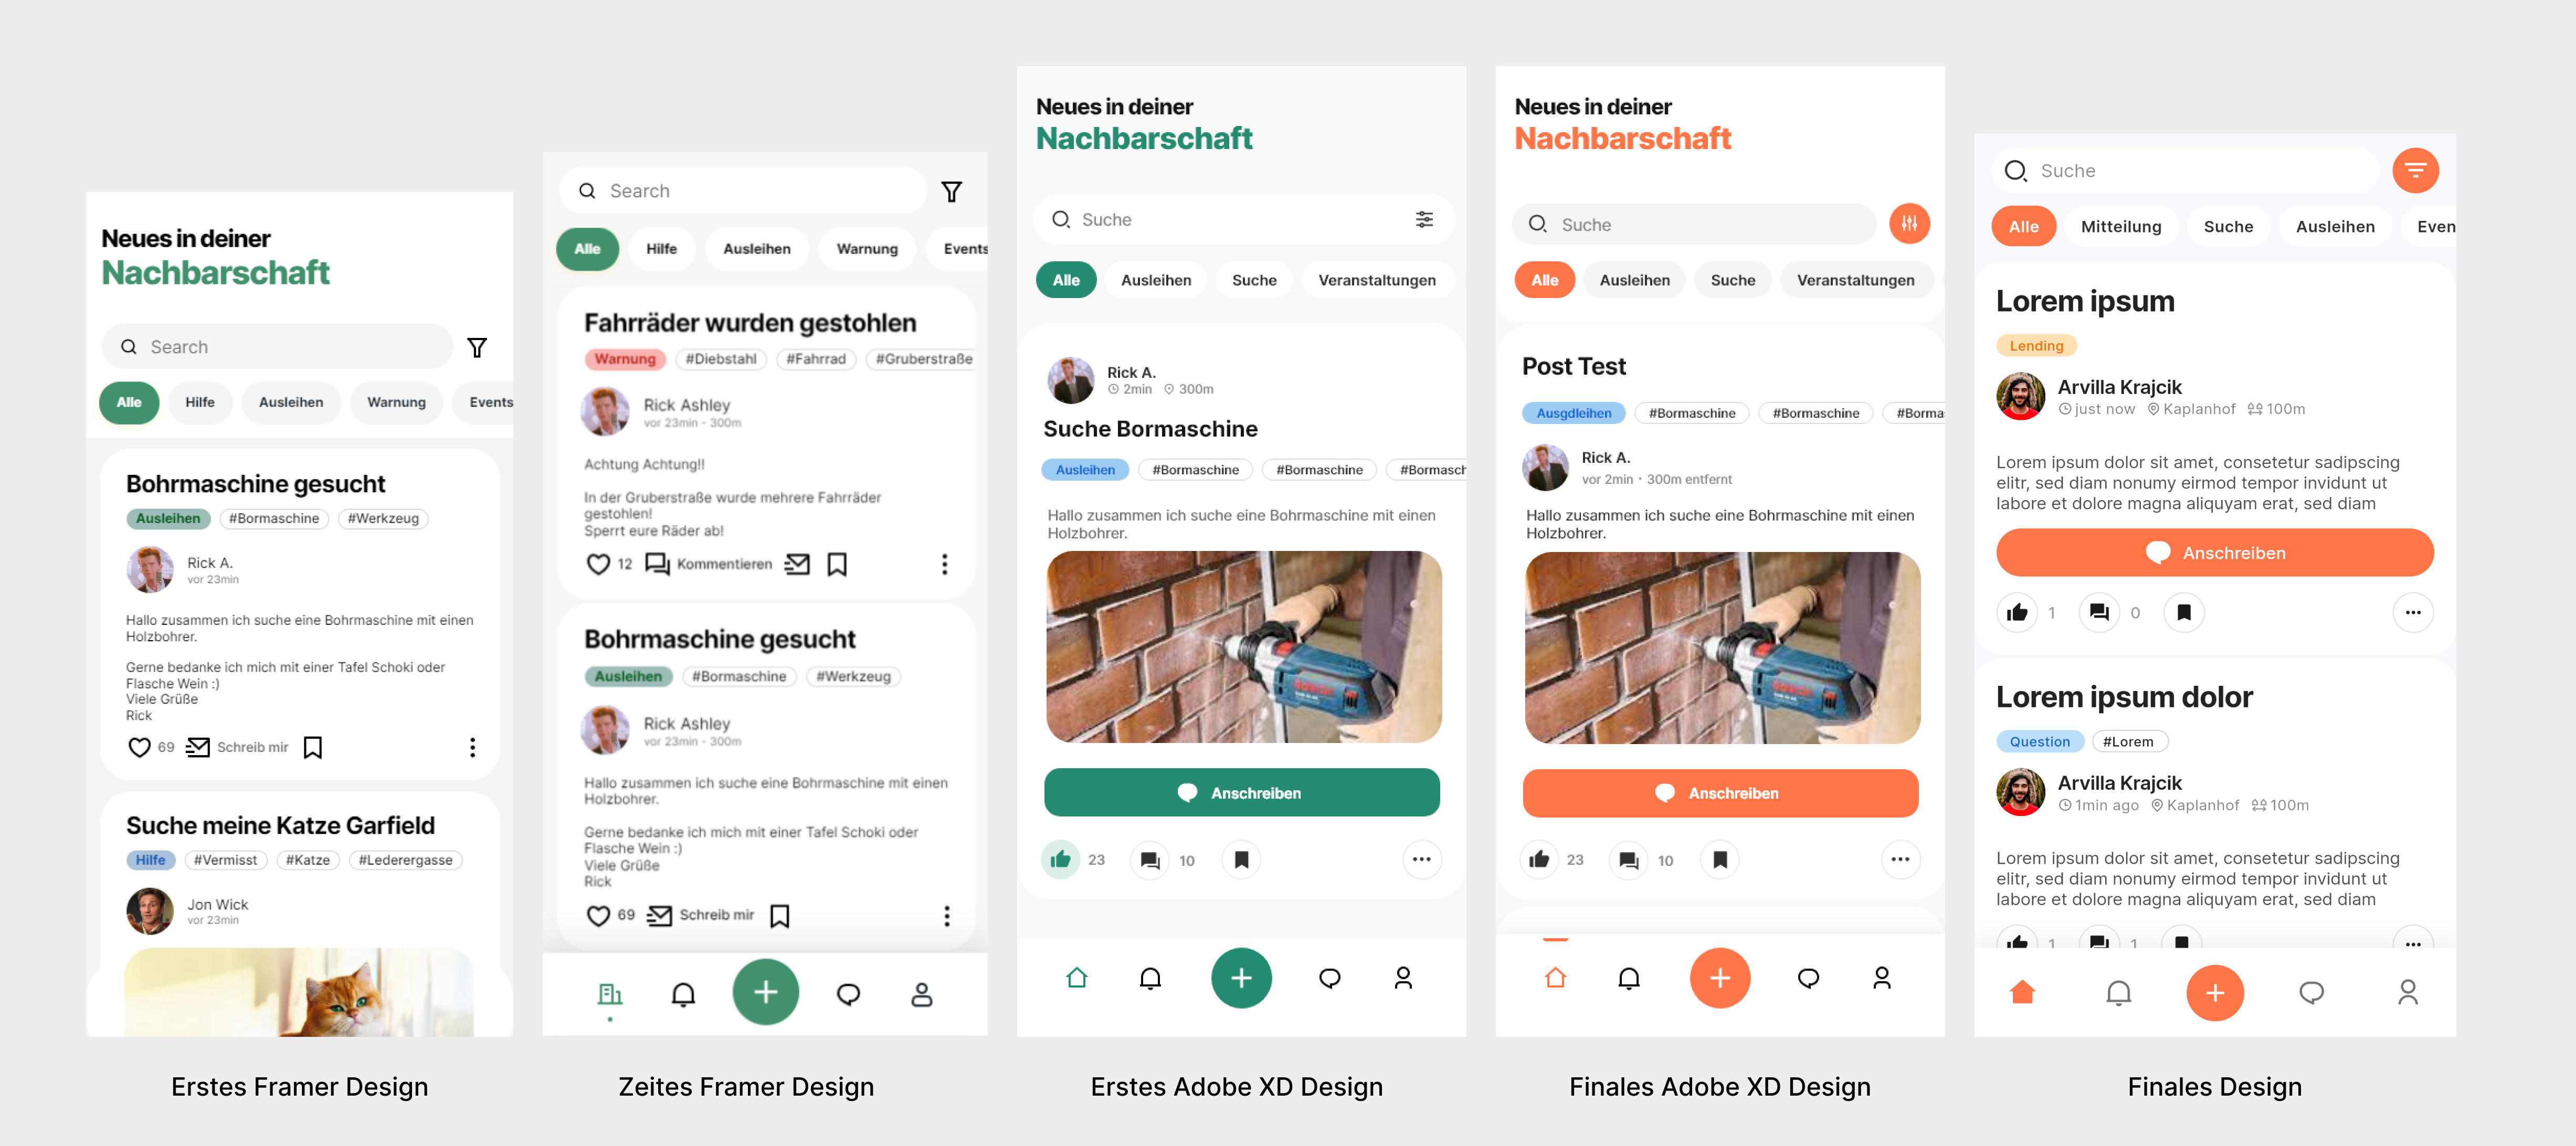
\includegraphics[width=1\textwidth]{pics/app-design-history.png}
  \caption{Screenshots verschiedener Versionen des App-Home-Screen}
  \label{fig:app-design-history}
\end{figure}
Im Rahmen des Hackathons Linz haCKt wurde das erste Design in Abbildung \ref{fig:app-design-history} ganz links erstellt. Hierbei wurden mehrere Brainstorming-Meetings mit Mentoren abgehalten, um ein Grundkonzept in Adobe XD zu gestalten. Anschließend wurden die groben Züge des Designs in Absprache mit dem Team festgelegt. Ein funktionsfähiger Prototyp wurde in Framer erstellt und am Tag der Endpräsentationen vorgestellt und verlinkt. Nach Linz haCKt wurde das zweite Design in Framer entwickelt.

Zwischen dem zweiten Framer-Design
\ref{fig:app-design-history} und dem ersten Adobe XD-Design
\ref{fig:app-design-history} wurde bewusst kein Abstand am
Rand eines Beitrags gehalten, um den vollen Handy-Display
auszunutzen. Der Filter-Button wurde mit der Suchleiste
verbunden, um das Design stimmiger zu gestalten. Bei den
Profilinformationen wurde auf Icons umgestellt, um es für
neue Nutzer verständlicher zu machen. Diese Entscheidung
wurde kurzzeitig verworfen, jedoch später in der Flutter-App
wieder eingebaut.

Wie man erkennen kann, wurde für das Finale Adobe
XD-Design \ref{fig:app-design-history} eine orangene Farbe für die Kapitelfarben
gewählt. Der letzte Screenshot zeigt die Flutter-App, wie
sie im Play Store erhältlich ist. Die größte Änderung
gegenüber dem vorherigen Design betrifft den Hintergrund
bei der Suche und der Kategorieauswahl. Der Hintergrund
wurde hellgrau gemacht, um die Beiträge besser hervorzuheben.
Bei der Entwicklung mit Flutter stellte sich heraus, dass
ein Strich über dem aktiven Icon sehr aufwändig zu
implementieren ist, weshalb darauf verzichtet wurde.



\section{Website}
\setauthor{Martin Hausleitner}
\begin{figure}[h]
  % \centering
  
\includegraphics[width=1\textwidth]{pics/website-design.png}
  \caption{Screenshot der Nochba Website: nochba.at}
\end{figure}

Die Medienpräsenz des Projekts, die durch die Teilnahme an Linz hACkT erlangt wurde, und das Fehlen eines zentralen Anlaufpunkts für Informationen führten zur Entscheidung, eine einfache Landing Page zu erstellen. Diese Seite bietet grundlegende Informationen und ist unter \href{https://nochba.at}{nochba.at} erreichbar.

Die Teilnahme am mPreneur Social Mobile Entrepreneurship von Arsham Edalatkhah führte zu internationaler Aufmerksamkeit für das Projekt. Dies veranlasste die Erstellung einer englischsprachigen Website unter \href{https://nochba.com}{nochba.com}. Ziel ist es, die Arbeit einem breiteren Publikum zugänglich zu machen und die Reichweite des Projekts zu erhöhen. Durch die Präsenz in einer internationalen Sprache kann das Interesse von Menschen aus verschiedenen Ländern und Kulturen geweckt und potenziell eine größere Nutzerbasis erreicht werden.


\subsection{Beta-tester anmeldung}
Das wichtigste Merkmal der Website ist die Option für Nutzer, sich für die Testphase zu registrieren. Ursprünglich wurde versucht, die E-Mail-Adressen der Nutzer über die Google Sheets API zu speichern. Allerdings erwies sich dieser Ansatz als ineffektiv und dauerte mehrere Stunden. Als Alternative wurde das Framer-Add-On von Mailchimp.com genutzt, um Zeit zu sparen. Der kostenlose Plan von Mailchimp war für die Bedürfnisse ausreichend. Stand 7.3.2023 wurden 34 Beta-Anmeldungen über das Formularfeld gesammelt.


\subsection{Design}
Für die Gestaltung der Landing Page ließ sich der Designer
von den Vorlagen von Framer inspirieren und nutzte
vorgefertigte Abschnitte. Diese wurden jedoch so
modifiziert, dass sie dem Designsysten gerecht werden. Die
Farbpalette wurde beibehalten und es wurde darauf geachtet,
dass die Website möglichst einfach gestaltet ist.

\subsection{Kontent}
Auf der Website sind folgende Informationen abgebildet:
\begin{itemize}
  \item Zeitungsartikel
        \begin{itemize}
          \item \href{https://www.meinbezirk.at/linz/c-wirtschaft/linzer-nachwuchs-hacker-beweisen-sich-in-nordmazedonien_a5654095}{Mein Bezirk}
          \item \href{https://www.linz.at/medienservice/2022/202203_114704.php}{Linz}
          \item \href{https://www.nachrichten.at/oberoesterreich/linz/von-linz-nach-nordmazedonien;art66,3728292}{OÖNachrichten}
          \item \href{https://jugendhackt.org/video/nochba/}{DorfTV}
          \item Kronen Zeitung (nur auf Papier)
        \end{itemize}
  \item Unsere Mission
  \item Beitrag Kategorien
  \item Auszeichnungen
        \begin{itemize}
          \item Immotopia Innovation Award
          \item mPreneur Austria
          \item Linz hACkt
        \end{itemize}
  \item Features der App
  \item Partner der Diplomarbeit
  \item Über uns
  \item Links
        \begin{itemize}
          \item \href{https://github.com/Martin-Hausleitner/Nochba}{Github Repo}
          \item \href{https://www.instagram.com/nochba.at/}{Instagram}
          \item Email \href{mailto:project@nochba.com}{project@nochba.com}
        \end{itemize}
\end{itemize}


\subsection{Hosting}
Die Website wurde mithilfe von \href{https://framer.com}{Framer} erstellt und auf deren
Hosting-Plattform gehostet. Um die Domain-Namen zu nutzen,
die über \href{https://www.godaddy.com/de-at}{GoDaddy} (nochba.at und nochba.com) gekauft wurden, wurde eine Weiterleitung
mit Maskierung auf die entsprechende Framer-URL
eingerichtet. Durch diese Maßnahme wurde im Browser bei der
URL die gekaufte Domain angezeigt.

\subsubsection{SSL-Zertifikat}
Aktuell verfügt die Website über kein SSL-Zertifikat, da durch die Maskierung das Framer SSL-Zertifikat entfällt. Dennoch wird die Website im Browser nicht als bedrohlich eingestuft. Aus diesem Grund wurde entschieden, kein SSL-Zertifikat zu erstellen und somit den Aufwand zu reduzieren.

\section{Backend}

\subsection{Firebase}
\setauthor{Martin Hausleitner}
Firebase ist ein Backend-as-a-Service (BaaS), das Entwicklern eine enorme Erleichterung bei der Arbeit bietet. Das Hosting von Datenbanken und Cloud-Funktionen kann mit nur wenigen Klicks erfolgen, was die Notwendigkeit von Skalierung oder Ausfallvermeidung eliminiert. Das Firebase-Backend wird auf der Google Cloud in Frankfurt (EUR3 Europe-West) gehostet, um eine niedrige Latenz zu gewährleisten. Der kostenlose Spark-Plan war für den Gebrauch ausreichend, als der Dienst noch nicht die Firebase-Cloud-Funktionen genutzt hat. Um Kosten zu sparen, wurde lange Zeit mit dem Firebase-Emulator an den Cloud-Funktionen gearbeitet. Im Januar 2023 wurde auf den Blaze-Plan umgestiegen, um die Firebase-Cloud-Funktionen nutzen zu können. Bis März 2022 wurden nur wenige Euro für den Verbrauch gezahlt. Die Dokumentation und Tutorials von Firebase sind exzellent und es gibt viele Ressourcen auf YouTube.


\subsection{Firebase SDKs}
\setauthor{Sandin Habibovic}
Firebase SDK ist eine Sammlung von Software Development Kits, die von Firebase bereitgestellt werden, um Cloud-basierte Anwendungen zu erstellen.
Firebase SDK ist für eine Vielzahl von Programmiersprachen verfügbar, darunter JavaScript, Swift, Kotlin, Java und unter anderem Dart von Flutter.
Die Firebase SDK bietet eine breite Palette von Funktionen, mit denen leistungsstarke Anwendungen erstellt werden können, darunter Authentifizierung, Cloud Messaging, Cloud Firestore, Realtime Database, Cloud Functions. Mit diesen Funktionen können schnell und einfach Funktionen wie Benutzerverwaltung, Datenverwaltung, Messaging und Benachrichtigungen in Anwendungen integriert werden. Außerdem gibt es zu Firebase SDK eine umfangreiche Dokumentation und Support-Tools.

\subsection{Firebase Authentication}
\setauthor{Sandin Habibovic}
Email und Passwort authentication

\subsection{Cloud Firestore}
\setauthor{Sandin Habibovic}
NoSQL-Database, Dokument-basierte Speicherung, Subcollections
\subsection{Cloud Storage}
\setauthor{Sandin Habibovic}
Speicherung von Profilbilder und Post-Bilder
\subsection{Firebase Cloud Functions}
\setauthor{Martin Hausleitner}
Firebase Cloud Functions sind eine großartige Möglichkeit,
um Business-Logik abzubilden. Es handelt sich um serverlose
Funktionen, die in JavaScript oder TypeScript geschrieben
werden und einzeln auf der Google Cloud gehostet werden. Je
nach Nachfrage werden sie automatisch skaliert oder komplett
abgeschaltet. Ein Nachteil ist, dass die Startup-Zeit länger
sein kann als bei einem herkömmlichen Backend, das immer
läuft. Allerdings kann man durch Cloud Functions viel Geld
sparen, da nur die Prozessorlaufzeit bezahlt werden muss.

Firebase Cloud Functions ermöglichen es Entwicklern, auf verschiedene Ereignisse in Firebase-Produkten zu reagieren. Zum Beispiel, wenn sich Daten in der Firestore-Datenbank ändern oder ein neuer Nutzer in Firebase Authentication registriert wird. Wenn ein solches Ereignis eintritt, wird die entsprechende Cloud Function automatisch ausgeführt.

Alle Cloud Functions wurden in TypeScript entwickelt, da diese Programmiersprache Typsicherheit und verbesserte Fehlererkennung bietet.


\subsubsection{Registrierung mit einem Verifizierungscode}\label{subsec:registrierung-verify}
\setauthor{Martin Hausleitner}

Die Cloud-Funktion \texttt{checkVerificationCode} wird ausgeführt, wenn ein Nutzer sich mit einem Verifizierungscode registrieren möchte. Wenn der Benutzer nicht authentifiziert ist, wird eine \texttt{HttpsError} ausgelöst. Dann wird der Verifizierungscode überprüft, um sicherzustellen, dass er die korrekte Formatierung hat. Wenn der Code ungültig ist, wird eine weitere \texttt{HttpsError} ausgelöst.

Als Nächstes wird der Verifizierungscode mit der Datenbank abgeglichen, um sicherzustellen, dass er aktiv und noch nicht zu oft verwendet wurde. Wenn der Code erfolgreich validiert wird, wird die Adresse des Benutzers abgerufen und deren Koordinaten mithilfe einer API call an OpenStreetMap mit der Funktion \texttt{getOSMCoordinatesFromAddress} ermittelt. Dann wird die Entfernung zwischen der Adresse des Benutzers und der Adresse, die dem Verifizierungscode zugeordnet ist, berechnet mit der Funktion \texttt{getDistanceFromLatLonInMeters}. Wenn die Entfernung nicht innerhalb des zulässigen Bereichs liegt, wird eine weitere \texttt{HttpsError} ausgelöst.

Schließlich werden die Informationen des Benutzers und des Verifizierungscodes in der Datenbank aktualisiert, um anzuzeigen, dass der Benutzer erfolgreich verifiziert wurde. Die Cloud-Funktion gibt \texttt{true} zurück, um anzuzeigen, dass die Verifizierung erfolgreich war.

In jeder Phase der Funktion wird ein Logger verwendet, um Informationen über den Status der Funktion zu protokollieren.

\subsubsection{Regestrierung mit Gerät Koordinaten}
\setauthor{Martin Hausleitner}

Die Cloud-Funktion \texttt{checkAddressWithDeviceLocation} erfordert eine authentifizierte Anfrage und erhält eine Adresse sowie Längen- und Breitengradkoordinaten vom Gerät des Benutzers. Die Funktion prüft, ob alle erforderlichen Daten vorhanden sind und ruft dann die Funktion \texttt{getOSMCoordinatesFromAddress} auf, um die Koordinaten der angegebenen Adresse zu erhalten. Es wird auch die Funktion \texttt{getDistanceFromLatLonInMeters} aufgerufen, um die Entfernung zwischen der Adresse und den Koordinaten des Geräts des Benutzers zu berechnen.

Wenn die Entfernung größer ist als ein vordefinierter maximaler Abstand, wird eine Fehlermeldung ausgegeben und die Funktion gibt \texttt{false} zurück. Andernfalls speichert die Funktion die Koordinaten der Adresse und die Entfernung zwischen den Koordinaten des Geräts des Benutzers und der Adresse in der Firestore-Datenbank. Die Funktion ruft auch die Funktion \texttt{getOSMSuburbFromCoords} auf, um den Vorort der Adresse zu erhalten, und speichert diesen ebenfalls in der Firestore-Datenbank.

Die Funktion gibt \texttt{true} zurück, wenn die Verifizierung erfolgreich abgeschlossen ist.

In jeder Phase der Funktion wird ein Logger verwendet, um Informationen über den Status der Funktion zu protokollieren.

\subsubsection{Verifizierungscode generieren}
\setauthor{Martin Hausleitner}
Die Cloud-Funktion \texttt{generateVerificationCode} definiert Konstanten für das Intervall zwischen der Generierung von Codes, die maximale Anzahl von Codes und die Reichweite in Metern.

Anschließend wird der letzte Code des Nutzers aus der Datenbank geholt, um zu überprüfen, ob seit dem letzten generierten Code ausreichend Zeit vergangen ist. Wenn ja, wird der zuletzt generierte Code zurückgegeben.

Wenn nicht, wird eine Schleife gestartet, um einen neuen Code zu generieren mit der Funktion \texttt{generateRandomVerificationCode}. Der generierte Code wird dann mit Firestore abgeglichen, um sicherzustellen, dass er nicht bereits verwendet wurde.

Wenn der generierte Code eindeutig ist, wird überprüft, ob der Benutzer verifiziert ist. Wenn dies nicht der Fall ist, wird ein Fehler zurückgegeben. Andernfalls wird der generierte Code in die Firestore-Datenbank eingefügt, um den letzten generierten Code und das Datum der Generierung zu speichern.

Das Skript gibt dann den generierten Code zurück. In jeder Phase der Funktion wird ein Logger verwendet, um Informationen über den Status der Funktion zu protokollieren.

\subsubsection{Koordienaten von einer Adresse bestimmen}
\setauthor{Martin Hausleitner}
Für die Verifizierung ist es von Bedeutung, die Adresse des Nutzers in Koordinaten umzuwandeln, um im Backend damit arbeiten zu können. Ursprünglich wurde die Google Geocode API verwendet, jedoch ist diese kostenpflichtig. Eine passendere Alternative, die besser zur Projektphilosophie passt, wurde gefunden: Nominatim. Nominatim ist eine Open-Source-Geocoding-API für OpenStreetMap-Daten und bietet eine kostenlose API für diese spezielle Anforderung.

Die Funktion \texttt{getOSMCoordinatesFromAddress} nutzt die Bibliothek \texttt{axios}, um eine Anfrage an die Nominatim-API zu senden. Die API wird genutzt, um Koordinaten für eine Adresse zu erhalten.

Die Funktion nimmt einen Parameter \texttt{address} vom Typ \texttt{string} entgegen, welcher die Adresse enthält, für die Koordinaten abgerufen werden sollen.

Mithilfe von \texttt{axios.get} wird eine HTTP GET-Anfrage an die Nominatim-API gesendet. Die Adresse wird als URL-Parameter im Format \texttt{q=Adresse} übergeben. Die API liefert die Koordinaten als JSON-Objekt zurück, welches in der Variable \texttt{data} gespeichert wird.

Die Funktion überprüft dann, ob die Anfrage ein Ergebnis zurückgeliefert hat. Falls nicht, wird eine Fehlermeldung mit der Adresse ausgegeben.

Wenn ein Ergebnis vorhanden ist, wird das erste Ergebnis (in der Variable \texttt{firstResult}) verwendet, um eine neue Instanz der \texttt{GeoPoint}-Klasse zu erstellen. Diese Klasse ist Teil der Firebase-Admin-Bibliothek und ermöglicht die Speicherung von geografischen Koordinaten in einer Firestore-Datenbank.

\subsubsection{Entferung von zwei Nutzern berechnen}
\setauthor{Martin Hausleitner}
Die Cloud-Funktion \texttt{getDistanceFromTwoUsers} berechnet die Entfernung zwischen zwei Benutzern. Die Funktion erwartet eine \texttt{PostId} und einen authentifizierten Benutzer. Dann wird eine Überprüfung durchgeführt, ob der Post mit der angegebenen ID existiert und ob der Post eine gültige Reichweite hat. Es werden auch Überprüfungen durchgeführt, ob die Benutzerkoordinaten vorhanden sind, und ob die Entfernung zwischen beiden Benutzern innerhalb des Postbereichs liegt.

Die Funktion nutzt die importierten Funktionen \texttt{getDistanceFromLatLonInMeters} und \texttt{getNearestDistance}, um die Entfernung in Metern zu berechnen. Allerdings wird die berechnete Distanz grob gerundet, um die Privatsphäre der Nutzer zu wahren. Dabei werden die Längen- und Breitengradkoordinaten von zwei Benutzern miteinander verglichen, die aus der Firestore-Datenbank abgerufen werden. Wenn die Entfernung größer als die Reichweite des Posts ist, wird ein Fehler ausgegeben.

Schließlich gibt die Funktion die Entfernung zurück.

\subsubsection{Entfernung von zwei geographischen Koordinaten berechnen}
\setauthor{Martin Hausleitner}

\begin{lstlisting}[language=Java,caption=getDistanceFromLatLonInMeters Funktion,label=lst:getDistanceFunction]
    export function getDistanceFromLatLonInMeters(
        lat1: number,
        lon1: number,
        lat2: number,
        lon2: number
      ) {
        if (lat1 < -90 || lat1 > 90 || lon1 < -180 || lon1 > 180) {
          throw new Error(
            "Invalid coordinate: lat1 must be between -90 and 90, lon1 must be between -180 and 180"
          );
        }
        if (lat2 < -90 || lat2 > 90 || lon2 < -180 || lon2 > 180) {
          throw new Error(
            "Invalid coordinate: lat2 must be between -90 and 90, lon2 must be between -180 and 180"
          );
        }
        const R = 6371; // Radius der Erde in km
        const dLat = deg2rad(lat2 - lat1); // deg2rad unten
        const dLon = deg2rad(lon2 - lon1);
        const a =
          Math.sin(dLat / 2) * Math.sin(dLat / 2) +
          Math.cos(deg2rad(lat1)) *
            Math.cos(deg2rad(lat2)) *
            Math.sin(dLon / 2) *
            Math.sin(dLon / 2);
        const c = 2 * Math.atan2(Math.sqrt(a), Math.sqrt(1 - a));
        const d = R * c * 1000; // Distanz in Metern
      
        if (lat1 === lat2 && lon1 === lon2) return 0;
        return d;
      }
      
      function deg2rad(deg: number) {
        return deg * (Math.PI / 180);
      }
      
\end{lstlisting}
Der vorliegende Code \ref{lst:getDistanceFunction}
implementiert eine Funktion, die die
Distanz in Metern zwischen zwei geographischen Koordinaten
(Breitengrad und Längengrad) auf der Erdoberfläche
berechnet. Die Funktion nutzt die Haversine-Formel, welche auf Kugelgeometrie basiert und aus der Quelle \cite{movabletype} movabletype in Javascript übernommen wurde, um die kürzeste Entfernung zwischen zwei Punkten auf der Erdoberfläche zu berechnen.

Die Funktion \texttt{getDistanceFromLatLonInMeters} hat vier Parameter: \texttt{lat1} und \texttt{lon1} sind die Breiten- und Längengrade des ersten Punktes, während \texttt{lat2} und \texttt{lon2} die Breiten- und Längengrade des zweiten Punktes sind, zwischen denen die Distanz berechnet werden soll.

Zu Beginn des Codes werden die Eingabeparameter auf ihre Gültigkeit geprüft und eine Fehlermeldung wird ausgegeben, falls eine der Koordinaten außerhalb des Bereichs von \texttt{-90} bis \texttt{90} für die Breite und \texttt{-180} bis \texttt{180} für die Länge liegt.

Die Funktion berechnet dann die Differenzen der Breiten- und Längengrade sowie den Radius der Erde (\texttt{R}) in Kilometern. Die Differenzen werden dann in Radianten umgewandelt und die Haversine-Formel wird angewendet, um die Entfernung in Kilometern zu berechnen. Schließlich wird das Ergebnis in Meter umgewandelt und zurückgegeben.

Die Funktion \texttt{deg2rad} wird als Hilfsfunktion definiert, um Grad in Radianten umzurechnen.

Die Funktion gibt \texttt{0} zurück, falls die beiden Eingabeparameter denselben Wert haben, um zu vermeiden, dass eine sehr kleine Distanz als Ergebnis ausgegeben wird, wenn es sich um denselben Punkt handelt.


\subsubsection{Bestimmung der nächstgelegenen Entfernung}
\setauthor{Martin Hausleitner}
Zur Wahrung der Privatsphäre der Nachbarn ist eine Funktion erforderlich, die den nächstgelegenen Abstand zu den Nachbarn angibt, ohne den genauen Abstand offenzulegen. Diese Funktion trägt den Namen \texttt{getNearestDistance} und erhält einen Meterwert als Parameter.

Die Funktion erstellt ein Array mit den Optionen \texttt{[100, 200, 500, 1000, 5000, 10000, 15000]} und setzt die Variable \texttt{nearest} auf den ersten Wert im Array.

Dann wird eine Schleife ausgeführt, die durch jedes Element im Array \texttt{options} geht und prüft, welches Element am nächsten zum angegebenen Abstand \texttt{distance} liegt. Wenn ein Element näher ist als das bisher am nächsten liegende Element, wird \texttt{nearest} aktualisiert.

Letztendlich wird geprüft, ob \texttt{nearest} größer oder gleich 1000 ist. Abhängig davon wird der Abstand entweder in Kilometern oder Metern zurückgegeben. Ist der Abstand größer oder gleich 1000, wird die Einheit \texttt{km} hinzugefügt, andernfalls wird \texttt{m} verwendet. Verzichtet wurde bewusst auf Switches oder If-Bedingungen, da mit der aktuellen Funktion schneller Abstände geändert werden können. Die Evaluierung des Arrays mit den Optionen ist noch im Gange.


\subsubsection{Nachbarschaft von Nutzer bestimmen}
\setauthor{Martin Hausleitner}
Um den App-Nutzern ein besseres Verständnis der Nachbarschaften zu vermitteln, in denen ihre Nachbarn leben, wird bei jedem Benutzer die jeweilige Nachbarschaft angezeigt. Diese Information wird automatisch in der Datenbank gespeichert, sobald der Nutzer verifiziert ist. Zur Umsetzung dieser Funktion wird eine Methode eingesetzt, die die geografischen Koordinaten des Benutzers verwendet, um die entsprechende Nachbarschaft mithilfe der OpenStreetMap-API abzurufen:

Die Funktion heißt \texttt{getOSMSuburbFromCoords} und nimmt zwei Parameter entgegen: \texttt{lat} für die geografische Breite und \texttt{lon} für die geografische Länge des Benutzers. Diese Funktion gibt eine Promise zurück, die eine Zeichenfolge \texttt{String} mit dem Namen der Nachbarschaft des Benutzers enthält. Die Funktion verwendet die Axios-Bibliothek, um eine GET-Anfrage an die OpenStreetMap-API zu senden. Diese Anfrage enthält die geografischen Koordinaten des Benutzers und die gewünschte Zoomstufe \texttt{18}, um die Nachbarschaft zu finden. Wenn die Anfrage erfolgreich ist, gibt die Funktion den Namen der Nachbarschaft zurück, der aus den Daten extrahiert wird, die von der API zurückgegeben werden. Wenn der Name der Nachbarschaft nicht verfügbar ist, gibt die Funktion den Namen der Stadt oder der Gemeinde zurück, in der sich der Benutzer befindet. Wenn auch diese Informationen nicht verfügbar sind, gibt die Funktion \texttt{null} zurück. Wenn bei der Anfrage ein Fehler auftritt, wird eine Fehlermeldung ausgelöst.


\subsubsection{Verifizierungscode format überprüfen}
\setauthor{Martin Hausleitner}
Um die Laufzeit bei der Verifizierung von Cloud-Funktionen zu optimieren, ist es sinnvoll, am Anfang der Verifizierung eine Überprüfung durchzuführen, ob der Verifizierungscode das richtige Format hat. Dazu wird die Funktion \texttt{verifyVerificationCode} genutzt werden, welche einen \texttt{String} als Parameter erwartet und einen \texttt{Boolean}-Wert zurückgibt. In der Funktion wird ein regulärer Ausdruck Regex definiert, um sicherzustellen, dass der Verifizierungscode den Anforderungen entspricht. Der Regex lautet \texttt{/}\verb|^[a-zA-Z0-9]{10}$/|\texttt{,} was bedeutet, dass der Code aus genau 10 alphanumerischen Zeichen bestehen muss. Mit der Methode \texttt{checkVerificationCode} wird der übergebene Code auf Übereinstimmung mit dem Regex geprüft und das Ergebnis als \texttt{Boolean}-Wert zurückgegeben.

\subsubsection{Verifizierungscode generator}
\setauthor{Martin Hausleitner}

Die Funktion \texttt{generateRandomVerificationCode} erzeugt einen zufälligen Code mit einer Länge von 10 Zeichen, indem sie eine Kombination aus Groß- und Kleinbuchstaben des englischen Alphabets sowie Ziffern von 0 bis 9 verwendet. Dabei wird \texttt{Math.random()} zur Generierung einer Zufallszahl zwischen 0 und 1 genutzt und mit der Länge des Zeichenfolgen-Arrays multipliziert, um eine zufällige Position innerhalb des Arrays auszuwählen. Anschließend wird das ausgewählte Zeichen an das Ergebnis angehängt und dieser Schritt wird für jedes Zeichen wiederholt, bis eine Zeichenkette der Länge 10 generiert wurde.

Diese Funktion wird in der Cloud-Funktion \texttt{generateVerificationCode} verwendet, um einen zufälligen Code zu generieren. Es ist wichtig, dass der Code-Generator in der Lage ist, eine ausreichende Anzahl von Codes zu generieren, damit es keine Kollisionen gibt. Da jeder Code zufällig generiert wird und die Funktion eine zufällige Zeichenkette aus 62 möglichen Zeichen erzeugt, ist es äußerst unwahrscheinlich, dass der gleiche Code zweimal generiert wird. Die Anzahl der möglichen Kombinationen beträgt $62^{10}$, was ungefähr $8.39 \times 10^{17}$ Möglichkeiten entspricht. Daher ist die Wahrscheinlichkeit, dass zwei identische Codes generiert werden, vernachlässigbar.


\subsection{Algolia Search}
\subsection{Algolia SDK}

\subsubsection{Typesense Search}
\subsection{Typesense SDK}

\section{Visual Studio Code Extensions}
\setauthor{Martin Hausleitner}




\section{Email}
\setauthor{Martin Hausleitner}
Aufgrund des erhöhten E-Mail-Verkehrs des Teams nach dem Wettbewerb Linz haCKt musste eine Lösung gefunden werden, um diesen zentral zu verwalten. Aus diesem Grund wurde eine Gmail-Adresse erstellt, nämlich \href{mailto:project.locoo@gmail.com}{project.locoo@gmail.com}.

\subsection{Wechsel auf Nochba}
Als das Team von Locoo auf Nochba wechselte und eine .com- und .at-Domain erwarb, entstand die Idee, eine eigene E-Mail-Adresse zu erstellen. Beim Versuch, einen E-Mail-Server auf Azure selbst zu hosten, wurde schnell klar, dass dies nicht möglich war. Im Allgemeinen gestaltet sich das Hosten eines E-Mail-Servers schwierig, da viele Cloud-Anbieter dies nicht erlauben.

\subsection{Hosting-Anbieter}
Um den Aufwand zu minimieren, wurde der Hosting-Anbieter \href{https://www.namecheap.com/}{Namecheap} ausgewählt, der ein sehr günstiges Angebot für ein Jahr E-Mail-Hosting hatte, bestehend aus 2 Monaten gratis und einem Jahr zum Preis von \$8.93.

\subsection{E-Mail-Adresse und Google-Account}
Die Entscheidung fiel auf die E-Mail-Adresse
\href{mailto:project@nochba.com}{project@nochba.com}, die mit dem DNS verbunden wurde.
Gleichzeitig wurde ein Google-Account erstellt, um alles
einheitlich mit der neuen E-Mail-Adresse zu gestalten.

\subsection{Zugang und Nutzung}
Das gesamte Team hatte Zugang zur E-Mail-Adresse und zum Webmail-Zugriff, obwohl die E-Mail-Adresse hauptsächlich von Martin Hausleitner und Arsham Edalatkhah genutzt wurde.

\subsection{Vorteile}
Rückblickend erwies sich die Entscheidung, eine eigene
E-Mail-Adresse zu erstellen, als äußerst vorteilhaft. Sie
vermittelte einen professionellen Eindruck und führte dazu,
dass das Projekt ernster genommen wurde. Zudem erleichterte
die eigene E-Mail-Adresse die Verwaltung von E-Mails an
einem zentralen Ort. Dies war besonders praktisch, da im


Laufe des Projekts verschiedene Anfragen eingingen und so
die Kommunikation effizienter gestaltet werden konnte.


\section{Visual Studio Code Ext}

Für die Programmierung einer App wurde das Werkzeug ChatGPT
eingesetzt, das auch nach der Veröffentlichung von GPT-4relevanter wurde. Eine einfache VSCode-Erweiterung wurde
entwickelt, um den Dart-Code zu minimieren. Da GPT-4 jedoch
nur eine Eingabe von 8000 Tokens zulässt, ist es schnell
erreicht, wenn der Code nicht minimiert wird, insbesondere
wenn viele Leerzeichen aufgrund von Einrückungen vorhanden
sind. Jedes Leerzeichen stellt dabei ein Token dar, was
schnell zu einer Überschreitung der maximalen Tokenanzahl
führen kann. Die Erweiterung wurde vollständig von GPT-4
programmiert und ist unter \ref{copyminify}[https://github.com/Martin-Hausleitner/vscode-copyminify] verfügbar.

Später wurde eine weitere Erweiterung programmiert, die die Anzahl der Tokens im aktuellen Code-File mithilfe von Codex oder GPT-3 Tokenizer anzeigt. Wenn ein bestimmter Bereich im Code-File ausgewählt ist, wird nur die Anzahl der Tokens in diesem Bereich angezeigt. Die Erweiterung wurde ebenfalls im VSCode Marketplace veröffentlicht und ist unter \ref{GPT-3 & Codex Tokenizer}[https://marketplace.visualstudio.com/items?itemName=MartinHausleitner.vscode-tokenizer-gpt3-codex] erhältlich.



\section{Zukünftige mögliche implementierungen}
Das Ziel des Teams besteht darin, die App jedem Österreicher und jeder Österreicherin zugänglich zu machen, weshalb die Entwicklung noch lange nicht abgeschlossen ist. Aus diesem Grund wurden im Folgenden einige Ideen aufgelistet, die während des Brainstormings entstanden sind.


\begin{itemize}
  \item App soll komplett auf Open-Source-Plattformen basieren
  \item Neuentwicklung der App
  \item Supabase statt Firebase verwenden
\end{itemize}

\subsection{Benutzererfahrung (UX) und Benutzeroberfläche (UI)}
\begin{itemize}
  \item UI/UX-Überarbeitung
  \item Eigenes UI-Package für die App
  \item Vereinfachung der Beitragserstellung
  \item Automatische Kategorisierung von Beiträgen durch KI
  \item Anpassbare Benachrichtigungseinstellungen
  \item Erweiterte persönliche Daten im Profil
\end{itemize}

\subsection{Registrierung und Profil}
\begin{itemize}
  \item Vereinfachung des Registrierungsprozesses
        \begin{itemize}
          \item Adressen-Autocomplete
        \end{itemize}
  \item Identitätsverifizierung mit Ausweis
  \item Weitere Verifizierungsmöglichkeiten
\end{itemize}

\subsection{Kommunikation und Interaktion}
\begin{itemize}
  \item Neuentwicklung des Chats
        \begin{itemize}
          \item Gruppenchats
          \item Chat-Reaktionen
          \item Sprachnachrichten
          \item Beiträge in Chats versenden
          \item Google ML Kit Entity Extraction
          \item Chat-Übersetzung
          \item Erweiterte Anhangsoptionen: Standort
        \end{itemize}
  \item Punktesystem wie Karma auf Reddit, um fleißige Nachbarn zu belohnen
  \item Zusätzliche Karma-Belohnungen für Reaktionen
  \item Weitere Kategorien, z.B. Umfragen
  \item Übersicht aller Nachbarn in der Umgebung
  \item In-App-Moderation und Berichterstattung unangemessener Inhalte
  \item Integration von Veranstaltungskalendern und lokalen Events
  \item Nachbarschaftsprojekte und gemeinsame Aktivitäten vorschlagen
  \item Lokale Geschäfts- und Serviceempfehlungen
\end{itemize}

\subsection{Internationalisierung und Übersetzungen}
\begin{itemize}
  \item App in mehreren Sprachen übersetzen
  \item Automatische Übersetzung für alle Teile der App
\end{itemize}

\subsection{Hilfe und Support}
\begin{itemize}
  \item Erweiterte Hilfe und Tutorials
  \item Erweiterte Einstellungsmöglichkeiten
\end{itemize}

\subsection{Technische Verbesserungen}
\begin{itemize}
  \item Umfangreiches Caching in der App
  \item Erweitertes Caching
  \item Chat-Verschlüsselung
  \item Deep Links für jede Seite
  \item Einladecodes mit Links
\end{itemize}

\subsection{Sicherheit und Datenschutz}
\begin{itemize}
  \item Erweiterte Sicherheitsmechanismen
  \item Integration von Wetter- und Verkehrsinformationen
  \item Erweiterte Benachrichtigungsoptionen
\end{itemize}

